% Optimally you should use XeLaTeX to typeset it, using system fonts. If you use pdflatex, standard LaTeX sans fonts will be used instead.
%
% This makes use of some stock MultiMarkdown LaTeX boilerplate. Thanks go to Fletcher Penney for creating a useful and simple system to extend from.

\documentclass[oneside,article,14pt,dvipsnames]{memoir}

\usepackage{layouts}[2001/04/29]
\usepackage[svgnames]{xcolor}
\definecolor{coolgrey}{Hsb}{293, 0.0, 0.5}
\definecolor{plumbgrey}{Hsb}{314, 0.3, 0.5}
\definecolor{redgrey}{Hsb}{337, 0.31, 0.6}
\usepackage{verse}
\usepackage{wrapfig}
\usepackage{sectionbreak}
\usepackage{perpage} %the perpage package
\MakePerPage{footnote} %the perpage package command
\usepackage{xpatch}
\usepackage{fancyvrb}
\usepackage{graphicx}
\usepackage{booktabs}
\usepackage{tabulary}
%\usepackage{listings}
\usepackage[sort&compress]{natbib}
\usepackage[normalem]{ulem}
\usepackage{adjustbox}
\usepackage[esperanto]{babel}
\usepackage{amssymb}
\usepackage[acronym]{glossaries}
\usepackage[utf8]{inputenc}
\usepackage[labelformat=empty]{caption}
\usepackage{calligra}
\usepackage{tikz}
\usetikzlibrary{matrix,fit,chains,calc,scopes}            
\usepackage{tcolorbox}
\tcbuselibrary{skins}
\usepackage{auto-pst-pdf} %To compile psvectorian directly
\usepackage{psvectorian}
\usepackage[all]{nowidow}

\glstoctrue
\makeglossaries
\makeindex

\usepackage{pdfpages}
\usepackage[T1]{fontenc}
\usepackage{fontenc,unicode-math}
%\usepackage{fontspec}
\setmainfont[Ligatures=TeX]{TeX Gyre Schola}
%\usepackage{beton}
%\renewcommand{\bfdefault}{sbc}
\usepackage[scale=0.89]{tgheros} % Helvetica is too big


%	\renewcommand{\familydefault}{\sfdefault}
	\newcommand{\helvetican}{}
	\newcommand{\helveticanl}{}

% Body Text Formatting
\linespread{1.2}
\setlength{\abnormalparskip}{0em}
\setlength{\parindent}{1.5em}


% Footnotes
\setlength{\footmarkwidth}{1.8em}
\setlength{\footmarksep}{0em}
\footmarkstyle{\footnotesize{#1}.\hfill}
\setfootins{16pt}{16pt}
\setlength{\footnotesep}{16pt}


%
%	8.5 x 11 layout for memoir-based documents
%   As defined in the stock MultiMarkdown system
%
%%% need more space for ToC page numbers
\setpnumwidth{2.55em}
\setrmarg{3.55em}

%%% need more space for ToC section numbers
\cftsetindents{part}{0em}{3em}
\cftsetindents{chapter}{0em}{3em}
\cftsetindents{section}{3em}{3em}
\cftsetindents{subsection}{4.5em}{3.9em}
\cftsetindents{subsubsection}{8.4em}{4.8em}
\cftsetindents{paragraph}{10.7em}{5.7em}
\cftsetindents{subparagraph}{12.7em}{6.7em}

%%% need more space for LoF numbers
\cftsetindents{figure}{0em}{3.0em}

%%% and do the same for the LoT
\cftsetindents{table}{0em}{3.0em}

%%% set up the page layout
\settrimmedsize{\stockheight}{\stockwidth}{*}	% Use entire page
\settrims{0pt}{0pt}

% Comment out the following command and replace it with the second, below it, if you intend to use CriticMarkup's margin notes, or marginalia of any sort.
\setlrmarginsandblock{1in}{1in}{*}
% \setlrmarginsandblock{1in}{2.5in}{*}
\setulmarginsandblock{1in}{1in}{*}

\setmarginnotes{17pt}{1.5in}{\onelineskip}
\setheadfoot{\onelineskip}{2\onelineskip}
\setheaderspaces{*}{2\onelineskip}{*}
\checkandfixthelayout

\VerbatimFootnotes

% Section Headings
\setsecheadstyle{\helveticanl\LARGE\raggedright\textcolor{ForestGreen}}
\setsubsecheadstyle{\helveticanl\large\raggedright\textcolor{ForestGreen}}
\setsubsubsecheadstyle{\helveticanl\normalsize\raggedright\textcolor{ForestGreen}}

\maxsecnumdepth{chapter}
\setsecnumdepth{chapter}
\settocdepth{section}

% Spacing Model
% Use "negative" values for the beforeXskip settings; this indicates the following paragraph should have its indent suppressed.
\setbeforesecskip{-14pt}
\setaftersecskip{12pt}
\setbeforesubsecskip{-14pt}
\setaftersubsecskip{12pt}
\setbeforesubsubsecskip{-14pt}
\setaftersubsubsecskip{6pt}

% Chapter heading style
\makechapterstyle{modern-style}{
    \renewcommand*{\chaptitlefont}{\Huge\centering\normalfont}
    \renewcommand*{\chapnumfont}{\Huge\raggedright\mdseries}
	\renewcommand*{\chapnamefont}{\chapnumfont}
	\renewcommand*{\printchaptername}{\chapnamefont\color{ForestGreen}}
	\renewcommand*{\printchapternonum}{\chapnamefont\color{ForestGreen}}
	\renewcommand*{\printchapternum}{}
	\renewcommand*{\chapterheadstart}{\newpage \vspace*{4em}}

}
\chapterstyle{modern-style}

%\renewcommand*{\chapnumfont}{\Huge\raggedright\centering\color{ForestGreen}}
%\renewcommand*{\chapnamefont}{\chapnumfont}

% Part Breaks


\renewcommand{\partnamefont}{}
\renewcommand{\printpartname}{}
\renewcommand{\printpartnum}{}
\renewcommand{\partnumfont}{\partnamefont}
\renewcommand{\beforepartskip}{\null\vfil\thispagestyle{empty}}
\renewcommand{\midpartskip}{\par\vspace{6pt}}
% Comment the following line if you wish to print the name of the part
\renewcommand{\printparttitle}{\chapnamefont\centering\color{ForestGreen}}
\renewcommand{\afterpartskip}{\par\vspace{0pt}}


\renewcommand{\cftpartleader}{\cftdotfill{\cftdotsep}}
\renewcommand{\cftchapterleader}{\cftdotfill{\cftdotsep}}

\pagestyle{plain}
               
\renewcommand{\sectionbreak}{\fancybreak{\color{ForestGreen}\textbf{\star}}}
\def\mytitle{Ĉapelo de Sorĉisto}
\def\myauthor{Tove Jansson}
% Set up PDF
\usepackage[
	plainpages=false,
	colorlinks=true,
	urlcolor=ForestGreen,
	linkcolor=ForestGreen,
	citecolor=ForestGreen,
	filecolor=ForestGreen,
	pdfpagelabels,
	pdftitle={\mytitle},
	pagebackref,
	pdfauthor={\myauthor},
	bookmarksnumbered=true,
	bookmarksopen=true
	]{hyperref}
\hypersetup{bookmarksdepth=3}
\usepackage{memhfixc}

%
%	Configure information from metadata for use in title
%   Using default MultiMarkdown methods

\ifx\latexauthor\undefined
\else
	\def\myauthor{\latexauthor}
\fi

\ifx\subtitle\undefined
\else
%	\addtodef{\mytitle}{}{ \\ \subtitle}
	\expandafter\def\expandafter\mytitle\expandafter{\mytitle \\ \subtitle}
\fi

\ifx\affiliation\undefined
\else
%	\addtodef{\myauthor}{}{ \\ \affiliation}
	\expandafter\def\expandafter\myauthor\expandafter{\myauthor \\ \affiliation}
\fi

\ifx\address\undefined
\else
%	\addtodef{\myauthor}{}{ \\ \address}
	\expandafter\def\expandafter\myauthor\expandafter{\myauthor \\ \address}
\fi

\ifx\phone\undefined
\else
%	\addtodef{\myauthor}{}{ \\ \phone}
	\expandafter\def\expandafter\myauthor\expandafter{\myauthor \\ \phone}
\fi

\ifx\email\undefined
\else
%	\addtodef{\myauthor}{}{ \\ \email}
	\expandafter\def\expandafter\myauthor\expandafter{\myauthor \\ \email}
\fi

\ifx\event\undefined
\else
	\date[\mydate]{\today}
\fi

\ifx\latextitle\undefined
	\def\latextitle{\mytitle}
\else
\fi
 %   remove figure captions

% http://tex.stackexchange.com/a/58638/5764
\makeatletter
\def\ifemptyarg#1{%
	\if\relax\detokenize{#1}\relax % H. Oberdiek
	\expandafter\@firstoftwo
	\else
	\expandafter\@secondoftwo
	\fi}
\makeatother

\let\oldcaption\caption
\AtBeginDocument{%
	\renewcommand{\caption}[2][]{%
		\ifemptyarg{#2}{}{\oldcaption[#1]{#2}}%
	}%
}
\date{}

\renewcommand*{\psvectorianDefaultColor}{ForestGreen}%

\tcbset{
	Baystyle/.style={
		sharp corners,
		enhanced,
		boxrule=6pt,
		colframe=ForestGreen,
		height=0.9\textheight,
		width=0.9\textwidth,
		borderline={8pt}{-11pt}{},
	}
}


\title{\mytitle}
\author{\myauthor}

\begin{document}


\begin{tcolorbox}[Baystyle,]
	{\begin{center}
			\vspace*{0.14\textheight}
			\fontsize{45}{45}\scshape \mytitle\\        
			\vspace*{0.018\textheight}
			%\vspace*{0.2\textheight}
			% Big Logo\\
			\begin{center}

			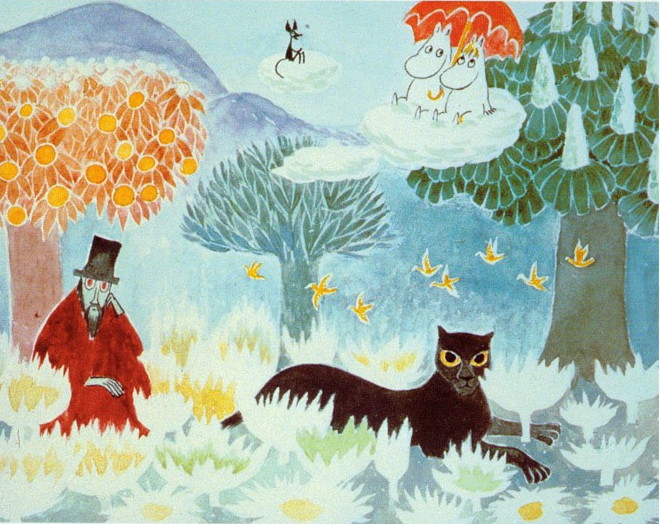
\includegraphics[width=0.5\textwidth]{cover.jpeg}
			\end{center}
			\vspace*{0.02\textheight}
			{\fontsize{12}{12}\calligra }
			\fontsize{28}{28}\scshape \myauthor\\
			\vspace*{0.1\textheight}
			\centering
			\begin{tikzpicture}[
				start chain=main going right,
				]
				\node[on chain,align=center,draw=none] (a1){{\fontsize{12}{12}\calligra %Illustrations by%
					} \\
					{\Large %Designer
					}
				}; 
				{ [start branch=A going below]
					\node[on chain,align=center,draw=none,scale=0.01](d1){};
					\node[on chain,align=center,draw=none,](d2){\Huge };
					%\node[on chain,align=center,draw=none,scale=0.01](d3){};
				}
				\node[on chain,align=center,draw=none,scale=1] (a2){\psvectorian[scale=0.3]{87}\psvectorian[scale=0.3,mirror]{87}}; 
				{ [start branch=B going below]
					\node[on chain,align=center,draw=none,scale=0.01](s1){};
					\node[on chain,align=center,draw=none,](s2){};
					%\node[on chain,align=center,draw=none,scale=0.01](s3){}; 
				}
				\node[on chain,align=center,draw=none]  (a3){{\fontsize{12}{12}\calligra %Final review by
					} \\
					{\Large %Revisor
					}
				};          
				{ [start branch=C going below]
					%\node[on chain,align=center,draw=none,scale=0.01](e1){};
					\node[on chain,align=center,draw=none,](e2){\Huge };
					%\node[on chain,align=center,draw=none,scale=0.01](e3){}; 
				}
				%\draw[black] (s2.north) -- (s2.south);
			\end{tikzpicture}
	\end{center}}
\end{tcolorbox}
\thispagestyle{empty}
\mainmatter
 

%\addcontentsline{toc}{chapter}{Mapo}
\thispagestyle{empty}
\setcounter{page}{2}
\vspace*{.5em}

\begin{figure}[htbp]
\centering
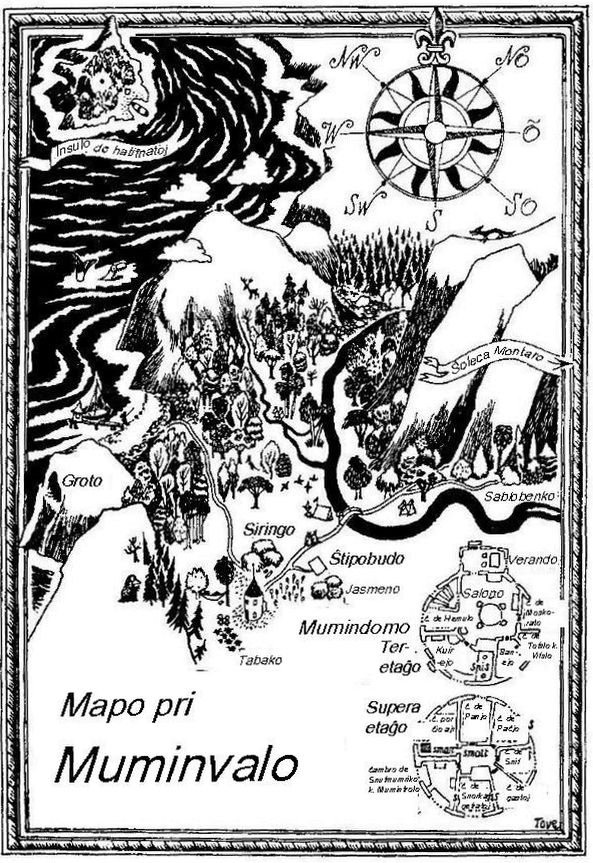
\includegraphics[width=401pt,height=585pt]{map-bildo.png}
\caption{}
\label{map-bildo}
\end{figure}

\chapter[Enhavo]{Enhavo}
\hypertarget{Enhavo}{}
\label{Enhavo}


\begin{figure}[htbp]
\centering
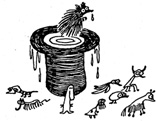
\includegraphics[width=117pt,height=90pt]{f000v-01.jpg}
\caption{}
\label{f000v-01}
\end{figure}

\begin{small}
\hyperref[Enkonduko]{Enkonduko}\hfill\pageref{Enkonduko}

\hyperref[Unua Ĉapitro]{Unua Ĉapitro}\hfill\pageref{Unua Ĉapitro}

\noindent\textit{en kiu oni priskribas kiel Mumintrolo, Snufmumriko kaj Snif trovis ĉapelon de sorĉisto, kiel neatendite aperis kvin nubetoj, kaj kiel la hemulo ekhavis novan hobion.}

\hyperref[Dua Ĉapitro]{Dua Ĉapitro}\hfill\pageref{Dua Ĉapitro}

\noindent\textit{en kiu oni rakontas kiel Mumintrolo transformiĝis en fantom-simion kaj finfine venĝis al la formikleono, kaj krome pri la sekreta nokta vagado de Mumintrolo kaj Snufmumriko.}

\hyperref[Tria Ĉapitro]{Tria Ĉapitro}\hfill\pageref{Tria Ĉapitro}

\noindent\textit{en kiu oni priskribas kiel la moskorato retiriĝis en dezerton kaj spertis ion nedireblan, kiel Aventuro portis la muminfamilion ĝis la soleca insulo de hatifnatoj kie la hemulo preskaŭ forbrulis kaj kiel la granda fulmotondro pasis super ili.}

\hyperref[Kvara Ĉapitro]{Kvara Ĉapitro}\hfill\pageref{Kvara Ĉapitro}

\noindent\textit{en kiu Snorkfraŭlino kalviĝas dum la nokta atako de hatifnatoj, kaj en kiu oni rakontas pri la ege mirigaj surstrandaj trovoj faritaj sur la soleca insulo.}

\hyperref[Kvina Ĉapitro]{Kvina Ĉapitro}\hfill\pageref{Kvina Ĉapitro}

\noindent\textit{en kiu oni parolas pri la Reĝa Rubeno, pri la fiŝado per longa hokarfadeno de la snorko kaj la morto de la mamluko, kaj pri kiel la mumindomo transformiĝis en ĝangalon.}

\hyperref[Sesa Ĉapitro]{Sesa Ĉapitro}\hfill\pageref{Sesa Ĉapitro}

\noindent\textit{en kiu Tofslo kaj Vifslo eniras la historion, kunportante misteran valizon kaj persekutate de la morho, kaj en kiu la snorko gvidas juĝoproceson}

\hyperref[Lasta Ĉapitro]{Lasta Ĉapitro}\hfill\pageref{Lasta Ĉapitro}

\noindent\textit{kiu estas tre longa kaj priskribas la foriron de Snufmumriko kaj kiel la mistera valiza enhavo estis malkaŝita, krome kiel la patrino de Mumintrolo rericevis sian mansakon kaj pro ĝojo aranĝis grandan festenon, kaj fine kiel la sorĉisto alvenis en Muminvalon.}

\end{small}

\chapter[Enkonduko]{}


\begin{figure}[htbp]
\centering
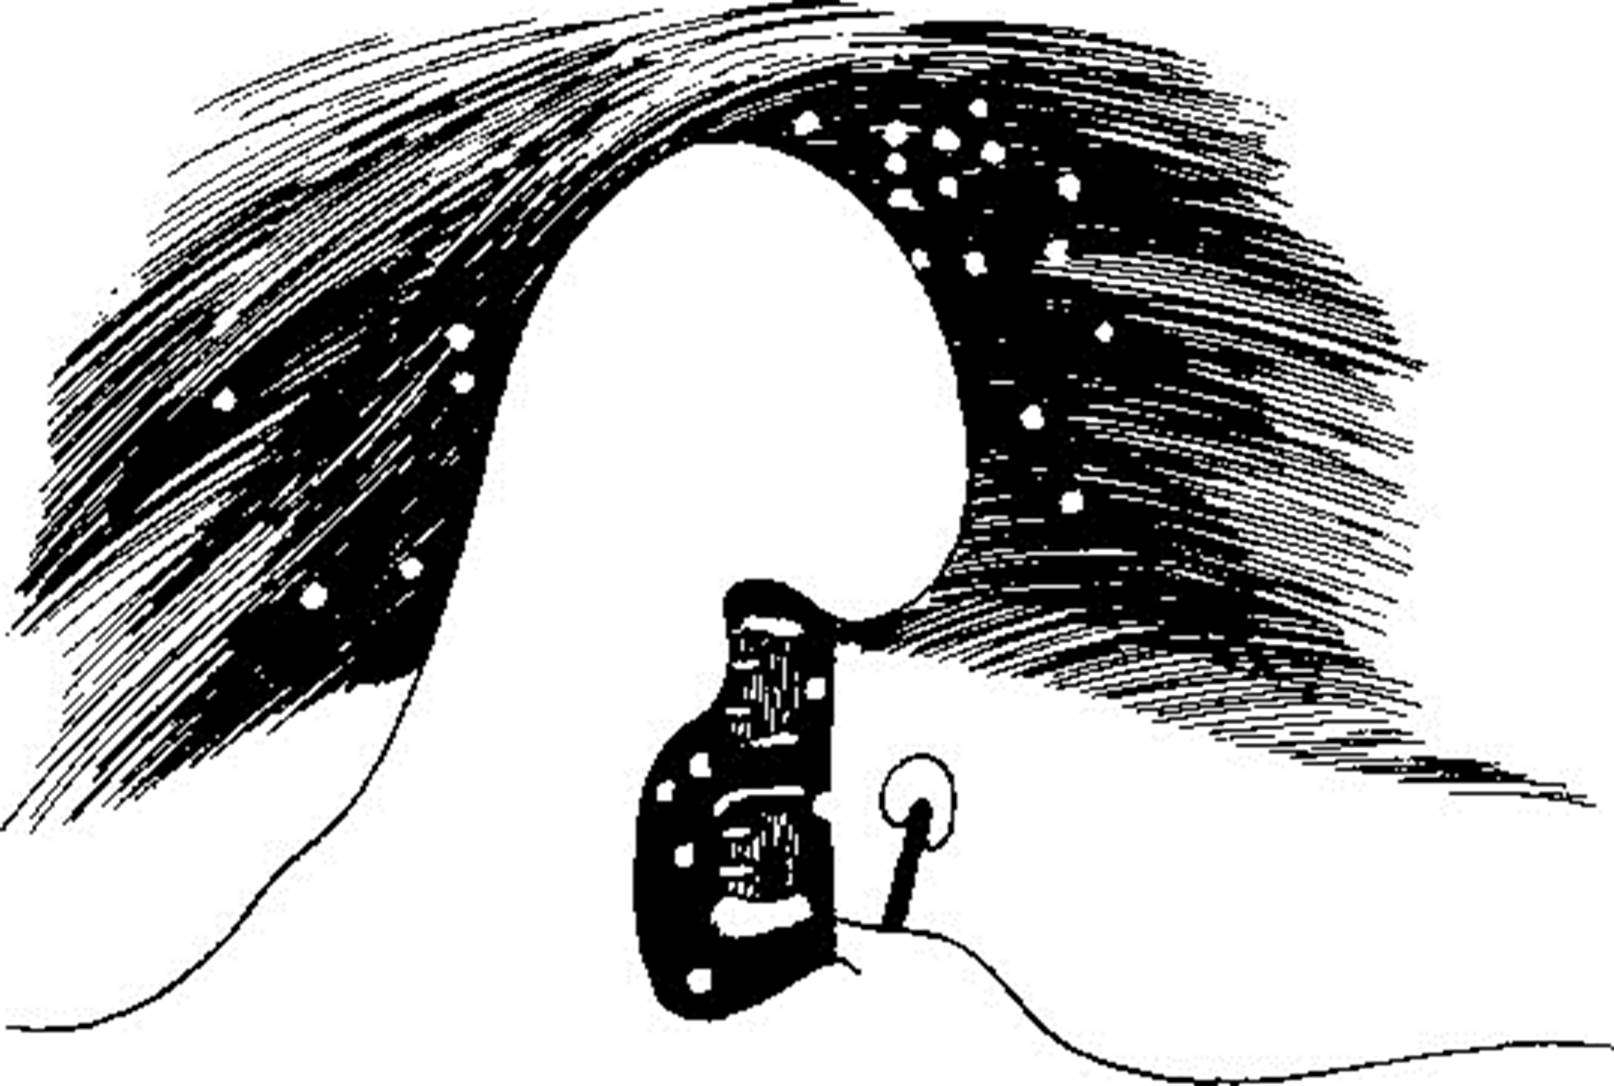
\includegraphics[width=400pt,height=268pt]{_1.jpg}
\caption{}
\label{_1}
\end{figure}

\begin{center}\textbf{\Large\color{ForestGreen}\textsc{Enkonduko}}\end{center}

\noindent En iu griza mateno la unua neĝo falis sur Muminvalon. Ĝi alŝteliĝis dense kaj silente, kaj post kelkaj horoj ĉio estis blanka.

Mumintrolo staris sur la ŝtuparo rigardante kiel la valo surmetas vintran littukon, kaj li kviete pensis: `Ĉi-vespere ni ekvintrodormos.' (Ĉar tiel ĉiuj mumintroloj kutimas fari iam en novembro kaj tio efektive estas sufiĉe prudenta faro de ĉiu kiu ne amas mallumon kaj froston). Li fermis la pordon kaj plandis ĝis sia patrino por diri:

``La neĝo alvenis.''

``Mi scias,'' diris la patrino de Mumintrolo. ``Mi jam sternis por vi ĉiuj la plej varmajn kovrilojn. Vi dormos en la okcidenta subtegmenta ĉambro kun la besteto Snif.''

``Sed Snif tiel terure ronkas,'' diris Mumintrolo. ``Ĉu mi ne povus anstataŭe dormi kun Snufmumriko?''

``Kiel plaĉas al vi,'' diris Muminpatrino. ``Snif povos dormi en la orienta ĉambro.''

Tiel la muminfamilio kaj ĉiuj iliaj amikoj kaj konatoj zorge kaj serioze preparis sin antaŭ la longa vintro. La patrino de Mumintrolo prezentis manĝon al ili en la verando, sed ĉiu ricevis nur piceajn pinglojn en sia taso (ĉar estas grave havi stomakon plenan de arbopingloj se oni intencas dormi dum tri monatoj). Kiam la vespermanĝo finiĝis (kaj ĝi ne tre bongustis) oni diris bonan nokton iom pli zorge ol kutime, kaj la patrino admonis ĉiujn lavi la dentojn.

Poste la patro de Mumintrolo rondiris por fermi ĉiujn pordojn kaj fenestrumojn kaj pendigi kulo-reton sur la lustron por ke ĝi ne polviĝu.

Kaj poste ĉiuj enlitiĝis, faris hejmecan kavon al si, tiris la kovrilon ĝis la oreloj kaj pensis pri io plaĉa. Sed Mumintrolo iom suspiris kaj diris:

``Ni tamen perdos amason da tempo!''

``Tute ne!'' diris Snufmumriko. ``Ni sonĝos. Kaj kiam ni revekiĝos estos printempo{\ldots}''

``Jes{\ldots}'' murmuris Mumintrolo. Li jam glitis foren en la duonkrepuskon de sonĝoj.

Eksterdome faladis neĝo, dense kaj delikate. Ĝi jam kovris la ŝtuparon, ĝi pendis peze sur tegmentoj kaj fenestraj kadrumoj. Baldaŭ la tuta mumindomo estos mola, ronda neĝamaso. La horloĝoj ĉesis tiktaki, unu post alia, la vintro alvenis.
\hfill \break
\hypertarget{Enkonduko}{}
\label{Enkonduko}


\chapter[Unua Ĉapitro]{}


\begin{figure}[htbp]
\centering
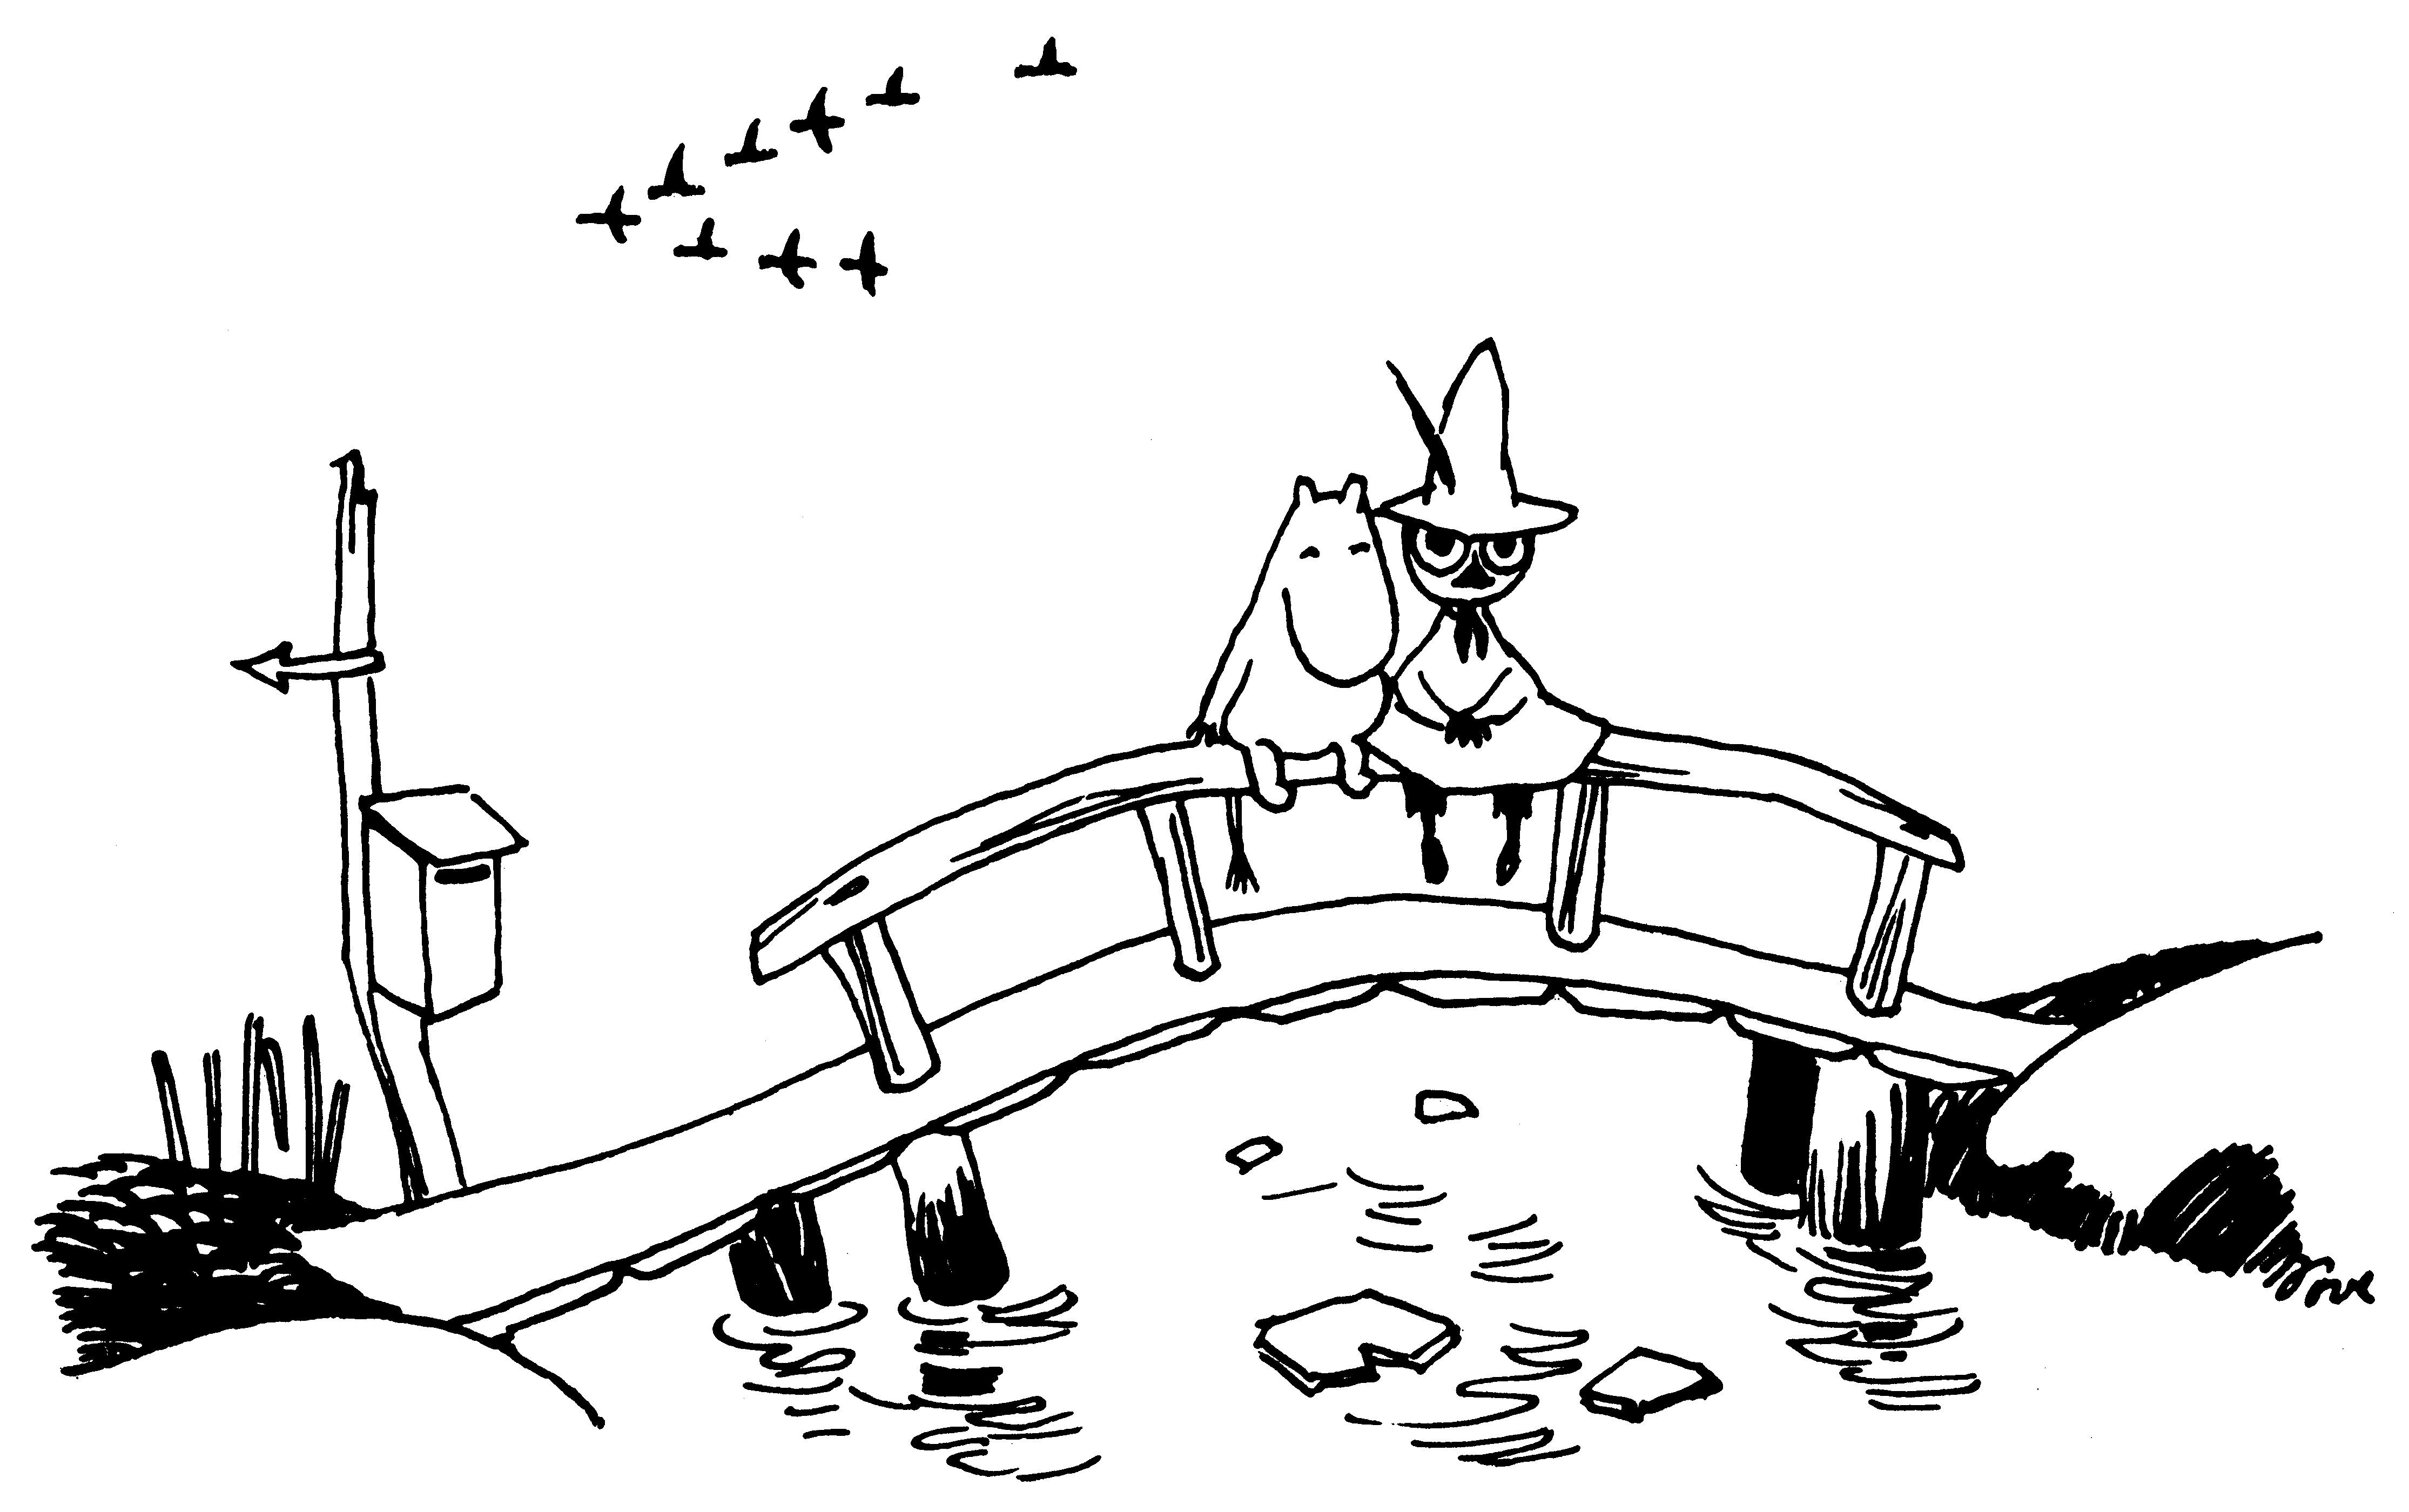
\includegraphics[width=399pt,height=251pt]{_2.jpg}
\caption{}
\label{_2}
\end{figure}

\begin{center}\textbf{\Large\color{ForestGreen}\textsc{Unua Ĉapitro}}\end{center}

\noindent\textit{en kiu oni priskribas kiel Mumintrolo, Snufmumriko kaj Snif trovis ĉapelon de sorĉisto, kiel neatendite aperis kvin nubetoj, kaj kiel la hemulo ekhavis novan hobion.}
\hfill \break
\hypertarget{Unua Ĉapitro}{}
\label{Unua Ĉapitro}


\noindent Iun printempan matenon je la kvara horo la unua kukolo flugis tra Muminvalo. Ĝi sidiĝis sur la tegmenton de la blua mumindomo kaj kukuis okfoje, ja iom raŭke, ĉar ankoraŭ estis tre frue printempe.

Poste ĝi flugis plu orienten.

Mumintrolo vekiĝis kaj longe kuŝis rigardante en la plafonon sen kompreni kie li troviĝas. Li dormis cent noktojn kaj cent tagojn, kaj la sonĝoj ankoraŭ kirliĝis ĉirkaŭ li kaj volis retiri lin en la dormon.

Sed kiam li turnis sin por trovi novan agrablan dormopozon li ekvidis ion kio tute klare vekis lin. La lito de Snufmumriko estis malplena.

Mumintrolo eksidis.

Jes, ankaŭ la ĉapelo de Snufmumriko estis for. ``Jen vere aĉa afero,'' diris Mumintrolo.

Li plandis ĝis la malfermita fenestro kaj rigardis eksteren. Jes ja, Snufmumriko uzis la ŝnuran ŝtupetaron. Mumintrolo trenis sin trans la fenestrobreton kaj singarde grimpis suben per siaj mallongaj kruroj. Li povis klare vidi la piedsignojn de Snufmumriko sur la malseka tero. Ili vagis tien-reen kaj estis sufiĉe malfacile sekveblaj. Jen kaj jen ili faris longajn saltojn kaj krucis sin mem. `Li ĝojis,' pensis Mumintrolo. `Jen li faris transkapiĝon, tio estas klara kaj evidenta.'

Subite Mumintrolo levis la kapon aŭskultante. Malproksime Snufmumriko ludis per sia buŝharmoniko, li ludis sian plej gajan melodion: `\emph{Ĉiuj bestetoj bantigas la voston}'. Mumintrolo ekkuris direkte al la muziko.

Malsupre ĉe la rivero li renkontis Snufmumrikon kiu sidis sur la ponta apogilo balancante la piedojn super la rivero, kun sia malnova ĉapelo tirita suben sur la oreloj.

``Saluton,'' diris Mumintrolo kaj sidiĝis apud lin.

``Saluton,'' diris Snufmumriko kaj ludis plu.

La suno apenaŭ atingis super la arbopintojn kaj lumigis iliajn vizaĝojn. Ili duonfermis la okulojn al ĝi, svingis la krurojn super la brila fluanta akvo kaj sentis sin senzorgaj kaj amikaj. Sur tiu rivero ili iam pli frue velis al multaj mirindaj spertoj. Kaj en ĉiu vojaĝo ili trovis novajn amikojn kaj kunvenigis ilin hejmen en Muminvalon. La gepatroj de Mumintrolo akceptis ĉiujn iliajn novajn konatojn same trankvile, ili nur enmetis pluajn litojn kaj faris la manĝotablon pli granda. Tiel la mumindomo iĝis svarma domo kie oni faris kion ajn oni emis kaj malofte zorgis pri la morgaŭo. Kelkfoje ja okazis tie ekscitaj kaj teruraj aferoj, tamen neniu havis tempon enui (kaj tio ja estis granda avantaĝo).

Kiam Snufmumriko atingis la lastan strofon de sia printempa kanto li enpoŝigis la buŝharmonikon kaj diris:

``Ĉu Snif vekiĝis?''

``Mi pensas ke ne,'' diris Mumintrolo. ``Li ĉiam dormas unu semajnon pli ol la aliaj.''

``Do ni veku lin,'' diris Snufmumriko decide kaj saltis de la ponta apogilo. ``Hodiaŭ ni devos fari ion nekutiman, ĉar estos bela tago.''

Sub la fenestro de la orienta subtegmenta ĉambro Mumintrolo signalis laŭ ilia sekreta sistemo: tri ordinaraj fajfoj kaj unu longa tra la manoj (kio signifas: `aferoj okazontaj'). Ili aŭdis ke Snif ĉesas ronki, sed nenio moviĝis tie supre.

``Ankoraŭfoje,'' diris Snufmumriko. Kaj ili signalis kun duobla forto.

Tiam la fenestro frape malfermiĝis.

``Mi dormas!'' kriis Snif ĉagrenite.

``Nun venu malsupren, kaj ne koleru,'' diris Snufmumriko. ``Ni intencas fari ion nekutiman.''

Tiam Snif glatigis siajn dumdorme ĉifitajn orelojn kaj malgrimpis laŭ la ŝnura ŝtupetaro (oni eble devus mencii, ke ili havis ŝnuran ŝtupetaron sub ĉiu fenestro ĉar paŝi en ŝtuparoj rabas tiom da tempo).

Efektive ŝajnis iĝi bela tago. La tero estis plena de ĵusvekitaj bestetoj kiuj dormis dum la tuta vintro kaj nun kuradis tien-reen por rekoni ĉion. Oni aerumis vestaĵojn kaj brosis la lipharojn kaj riparis siajn domojn kaj ĉiel preparis sin por la nova printempo.

De temp' al tempo ili haltis por rigardi domkonstruon aŭ aŭskulti kverelon (tiaj ja okazas sufiĉe ofte en la unuaj printempaj tagoj, ĉar oni povas havi tre malbonan matenan humoron kiam oni ĵus elrampis el la dormejo).

Jen kaj jen arbospirito sidis sur branĉo kombante sian longan hararon, kaj en la restanta neĝo ĉe la norda flanko de la arbotrunkoj musidoj kaj etaj knitoj fosis longajn tunelojn.

``Bonan printempon!'' diris maljuna kolubra sinjoro. ``Kaj kia estis la vintro?''

``Bona, dankon,'' respondis Mumintrolo. ``Ĉu vi bone dormis, sinjoro?''

``Jes, bone,'' diris la kolubro. ``Donu miajn salutojn al viaj gepatroj!''

Proksimume tiel ili parolis kun amaso da personoj kiujn ili renkontis. Sed ju pli alte sur la monton ili atingis, des malpli da vivuloj troviĝis, kaj fine ili vidis nur unu-du musinojn kiuj kuradis okupataj de printempa purigado.

Ĉie estis malseke.

``Aĉ, kiel malagrable,'' diris Mumintrolo kaj levis la piedojn alten el la degelanta neĝo. ``Ĉi tiom da neĝo neniam povas utili al mumintrolo. Tion diris Panjo.'' Kaj jen li ternis.

``Aŭskultu, Mumintrolo'', diris Snufmumriko. ``Mi ekhavis ideon. Kion vi pensas, ĉu ni iru ĝis la montopinto kaj starigu tumulon tie por montri ke neniu estis tie antaŭ ni?''

``Ni faru tion,'' kriis Snif kaj ekiris por atingi antaŭ la aliaj.

Surpinte printempa vento dancis libere en rondo kaj ĉirkaŭe oni vidis bluajn horizontojn. Okcidente situis la maro, oriente la rivero serpentis en Solecan Montaron, norde la grandaj arbaroj etendis sian printempan tapiŝon, kaj sude la fumo altiĝis el la mumindoma kamentubo, ĉar la patrino de Mumintrolo kuiris matenan kafon. Sed Snif vidis nenion el ĉio ĉi. Ĉar surpinte de la monto kuŝis ĉapelo -- nigra cilindra ĉapelo.

``Iu estis ĉi tie antaŭ ni!'' kriis Snif.

Mumintrolo levis la ĉapelon kaj rigardis ĝin. ``Ĝi estas tre bela,'' li diris. ``Eble ĝi konvenas al vi, Mumriko.''

``Ne, ne,'' diris Snufmumriko kiu amis sian malnovan verdan ĉapelon. ``Ĝi estas ege tro nova!''

``Eble Paĉjo dezirus ĝin,'' cerbumis Mumintrolo.

``Ni kunportu ĝin,'' diris Snif. ``Sed nun mi volas iri hejmen. Mia stomako kriegas por havi kafon. Ĉu ankaŭ la viaj?''

``Certe!'' diris Mumintrolo kaj Snufmumriko kun emfazo.

Tiel okazis kiam ili trovis ĉapelon de sorĉisto kaj kunportis ĝin hejmen, sen antaŭscii ke per tio ili igas Muminvalon ludejo de magio kaj strangaĵoj ĉiaspecaj{\ldots}

\begin{figure}[htbp]
\centering
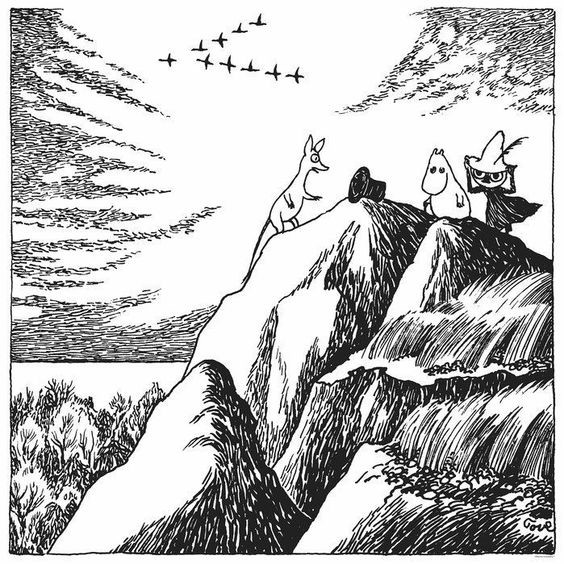
\includegraphics[width=406pt,height=406pt]{_3.jpg}
\caption{}
\label{_3}
\end{figure}

Kiam Mumintrolo, Snufmumriko kaj Snif venis en la verandon, la aliaj jam trinkis kafon kaj malaperis ĉiudirekten. Nur la patro de Mumintrolo restis legante la ĵurnalon.

``Nu bone, ĉu ankaŭ vi vekiĝis,'' li diris. ``Strange malmulte en la ĵurnalo hodiaŭ. Iu rivereto krevigis sian digon kaj pereigis formikejon. Ĉiuj estis savitaj. Plue la unua printempa kukolo traflugis la valon je la kvara kaj pluiris orienten.''

``Rigardu kion ni trovis,'' diris Mumintrolo fiere. ``Bela, nigra cilindra ĉapelo por vi!''

Muminpatro tre zorge esploris la ĉapelon kaj poste li surmetis ĝin antaŭ la salona spegulo. La ĉapelo estis iomete tro granda kaj ĝenis la vidadon, sed la tuta afero faris majestan impreson.

``Panjo!'' kriis Mumintrolo. ``Venu rigardi Paĉjon!''

La panjo malfermis la kuirejan pordon kaj haltis tre surprizite sur la sojlo.

``Ĉu ĝi konvenas al mi?'' demandis Muminpatro.

``Sendube ĝi konvenas,'' diris la patrino de Mumintrolo. ``Jes, vi aspektas tre vira kun ĝi. Nur{\ldots} ĝi ŝajne estas iomete tro granda.''

``Ĉu estas pli bone ĉi tiel?'' demandis la patro ŝovante la ĉapelon nuken.

``Hm,'' diris Muminpatrino. ``Ja estas bone, sed mi preskaŭ pensas ke vi aspektas pli digne sen ĉapelo.''

La patro spegulis sin de antaŭe, de malantaŭe kaj de flanke, poste li suspirante metis la ĉapelon sur la komodon.

``Vi pravas,'' li diris. ``Ne ĉio bezonas ornamon.''

``Gracio ornamas sin mem,'' diris la patrino de Mumintrolo amike. ``Manĝu pli da ovoj, idoj, vi vivis per arbopingloj dum la tuta vintro!'' Kaj jen ŝi reiris en la kuirejon.

``Sed kion ni faru el ĝi?'' demandis Snif. ``Tia bela ĉapelo!''

``Uzu ĝin kiel paperkorbon,'' diris la patro de Mumintrolo. Poste li retiriĝis en la supran etaĝon por verki siajn memorojn (la grandan libron kiu temas pri la ŝtorma junaĝo de Muminpatro).

Snufmumriko movis la ĉapelon surplanken inter la komodo kaj la kuireja pordo. ``Jen denove vi havas plian meblon,'' li diris rikanante, ĉar Snufmumriko malofte komprenis la ĝojon de posedo. Li bonfartis kun la malnova vesto kiun li surhavis de kiam li naskiĝis (neniu scias kie kajkiel), kaj la sola posedaĵo kiun li ne fordonis estis la buŝharmoniko.

\begin{figure}[htbp]
\centering
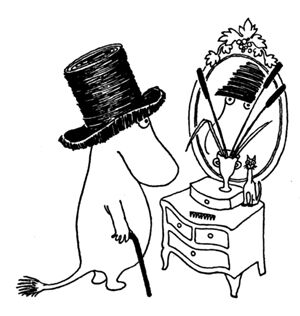
\includegraphics[width=150pt,height=157pt]{_4.jpg}
\caption{}
\label{_4}
\end{figure}

``Se vi jam finis matenmanĝi, do ni iru sperti kion la snorkoj faras,'' diris Mumintrolo. Sed antaŭ ol iri en la ĝardenon li forĵetis siajn ovoŝelojn en la paperkorbon, ĉar li (kelkfoje) estis ordema mumintrolo.

Poste la salono estis malplena.

En la angulo inter la komodo kaj la kuireja pordo staris la ĉapelo de sorĉisto kun ovoŝeloj surfunde. Kaj nun okazis io vere stranga. La ovoŝeloj komencis transformiĝi.

(La fakto estas, ke se io kuŝas sufiĉe longe en ĉapelo de sorĉisto, ĝi transformiĝas en ion tute alian -- precize kion, neniam eblas scii antaŭe. Estis feliĉo ke la patro de Mumintrolo ne trovis la ĉapelon konvena, ĉar se li konservus ĝin surkape iom pli longe nur la protektanto de ĉiuj bestetoj scias kio iĝus el li. Kiel nun okazis, li ekhavis nur malfortan kapdoloron -- kaj ĝi pasis jam posttagmeze).

Sed la ovoŝeloj restis en la ĉapelo, kaj malrapide ili komencis aliformiĝi. Ili konservis sian blankan koloron sed kreskis, kreskadis kaj iĝis molaj kaj lanaj. Post iom ili tute plenigis la ĉapelon. Kaj jen liberiĝis kvin etaj rondaj nuboj de la ĉapela rando kaj disŝvebis en la verandon, mole saltetis suben laŭ la ŝtuparo kaj restis enaere iom super la tero. Sed la ĉapelo de sorĉisto estis malplena.

``Kiel terure!'' diris Mumintrolo.

``Ĉu estas brulego?'' demandis la snorko maltrankvile.

Senmove la nuboj staris antaŭ ili, sen ŝanĝi formon, kvazaŭ atendante. Snorkfraŭlino tre singarde etendis la manon kaj tuŝis la plej proksiman nubeton. ``Ĝi sentiĝas kiel kotona vato,'' ŝi diris surprizite. La aliaj alproksimiĝis kaj palpis.

``Precize kiel kuseneto,'' diris Snif.

Snufmumriko delikate puŝetis unu el la nuboj. Ĝi glisis kelkan distancon kaj poste haltis denove.

``Kies ili estas?'' demandis Snif. ``Kiel ili venis en la verandon?''

Mumintrolo skuis la kapon. ``Jen la plej stranga afero kiun mi spertis,'' li diris. ``Eble ni devus venigi Panjon el la domo.''

``Ne, ne,'' vokis Snorkfraŭlino. ``Ni mem esploru ilin. Kaj ŝi tiris nubon suben sur la teron kaj glatumis ĝin permane. Kiel mole!'' diris Snorkfraŭlino. Kaj en la sekva sekundo ŝi sidiĝis sur la nubon kaj subridante balanciĝis supren-suben.

``Ankaŭ mi volas havi unu!'' kriis Snif kaj suriris alian nubon. ``Hej, hop!'' Sed kiam li diris ``hop!'' la nubo altiĝis kaj laŭiris elegantan arkon super la tero.

``Ĉielo!'' ekkriis Snif. ``Ĝi moviĝis!''

Nun ĉiuj saltis sur nubon kaj vokis ``hop! Hej, hop!'' La nubetoj forglisis tien-reen per longaj saltoj kvazaŭ obeemaj kunikloj. La snorko estis tiu kiu komprenis kiel oni stiras ilin. Malforta premo per unu piedo, kaj la nubo turniĝis. Per ambaŭ piedoj, plenrapide antaŭen. Skuetoj per la postaĵo, la nubo altiĝis ĝis oni sidis senmove.

Estis vere mirinde amuze. Ili kuraĝis iri eĉ supren ĝis la arbopintoj kaj sur la tegmenton de la mumindomo.

Mumintrolo surteriĝis per sia nubo ekster la fenestro de Muminpatro kaj kriis: ``Kokeriko!'' (li estis tiel ravita ke li ne eltrovis ion pli sencan).

Muminpatro lasis sian rakontplumon kaj ĵetis sin ĝis la fenestro.

``Je mia vosto!'' li ekkriis. ``Je mia vosto!'' Pli multe li ne povis eligi.

``Ĉi tio estos bela ĉapitro en viaj memoroj,'' diris Mumintrolo. Kaj poste li stiris sian nubon ĝis la kuireja fenestro kaj vokis la panjon. Muminpatrino okupiĝis kuiri miksofritaĵon kaj estis tre urĝata. ``Kion vi nun eltrovis, eta muminido,'' ŝi diris. ``Nur gardu vin ke vi ne falu!''

Sed sube en la ĝardeno la snorko kaj Snufmumriko elpensis ion novan. Ili stiris plenrapide unu kontraŭ la alia kaj kunpuŝiĝis per mola frapo. Kiu unue defalis, malvenkis.

``Nun vi spertos!'' kriis Snufmumriko kaj premis la piedojn en la flankojn de la nubo. Antaŭen!

Sed la snorko lerte cedis kaj poste ruze atakis de sube.

La nubo de Snufmumriko renversiĝis kaj li falis surkapen en la florbedon tiel ke lia ĉapelo premiĝis sur la nazon.

``Tria raŭndo!'' kriis Snif kiu estis juĝisto kaj flugis iom super la aliaj. ``Du kontraŭ unu! Atentu! Pretaj! Ek!''

``Ĉu ni faru etan flugon kune?'' Mumintrolo demandis Snorkfraŭlinon.

``Volonte,'' diris Snorkfraŭlino kaj stiris sian nubon apud la lian. ``Kien ni iru?''

``Eble ni elserĉu la hemulon por surprizi lin,'' proponis Mumintrolo.

Ili rondiris super la ĝardeno, sed la hemulo ne estis en siaj kutimaj lokoj.

``Kutime li neniam iras longe for,'' diris Snorkfraŭlino. ``Kiam mi lastfoje vidis lin, li ordigis siajn poŝtmarkojn.''

``Sed tio estis antaŭ duonjaro,'' atentigis Mumintrolo.

``Ej, jes ja!'' diris Snorkfraŭlino. ``Ni ja dormis de tiam.''

``Ĉu vi bone dormis?'' demandis Mumintrolo.

Snorkfraŭlino elegante flugis super arbopinto kaj iom cerbumis antaŭ ol respondi. ``Mi havis teruran sonĝon!'' ŝi diris. ``Abomena viro kun nigra ĉapelo rikanis al mi.''

``Kiel strange!'' diris Mumintrolo. ``Mi havis tute la saman sonĝon. Ĉu li krome portis blankajn gantojn?''

``Jes, ĝuste,'' diris Snorkfraŭlino kaj kapjesis.

Dum kelka tempo ili pensis pri tio glisante malrapide tra la arbaro. Subite ili ekvidis la hemulon kiu vagis antaŭen kun la manoj surdorse kaj la nazo direktita al la tero. Mumintrolo kaj Snorkfraŭlino glisis malsupren ĉiuflanke de li, kaj samtempe ili vokis: ``Bonan matenon!''

``Aĉ!'' ekkriis la hemulo. ``Fi, kiom mi ektimis! Vi scias ke oni devas ne subiti al mi, mi povus misgluti la koron!''

``Ej, pardonu,'' diris Snorkfraŭlino. ``Ĉu vi scias sur kio ni rajdas?''

``Estas io stranga,'' diris la hemulo. ``Sed mi tre kutimas je tio ke vi faras strangaĵojn. Kaj ĝuste nun mi melankolias.''

``Kial do?'' demandis Snorkfraŭlino kompate. ``En ĉi tia bela tago?''

La hemulo kapneis. ``Vi ĉiuokaze ne komprenus min,'' li diris.

``Ni provos,'' diris Mumintrolo. ``Ĉu vi refoje perdis mispresaĵon?''

\begin{figure}[htbp]
\centering
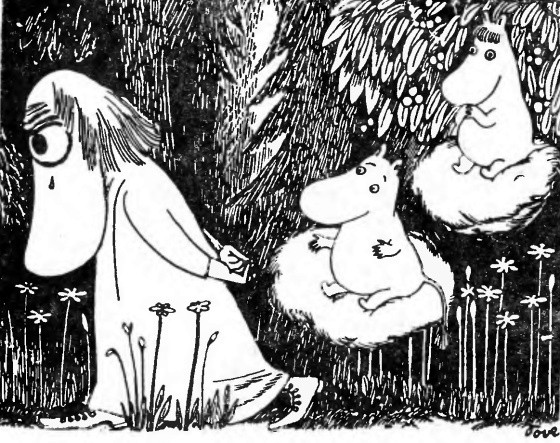
\includegraphics[width=420pt,height=332pt]{_5.jpg}
\caption{}
\label{_5}
\end{figure}

``Male,'' suspiris la hemulo. ``Mi havas ĉiujn. Ĉiun unuopan. Mia poŝtmarka kolekto estas kompleta. Nenio mankas en ĝi.''

``Nu, do!'' diris Snorkfraŭlino kuraĝige.

``Jes, mi ja sciis ke vi ne komprenos min,'' diris la hemulo.

Mumintrolo kaj Snorkfraŭlino zorgeme rigardis unu la alian. Ili lasis siajn nubojn iomete retroiri pro respekto al la malĝojo de la hemulo kaj pluiris malantaŭ lia dorso. La hemulo vagis plu dum Mumintrolo kaj Snorkfraŭlino atendis ke li parolu pri tio kio plenigas lian koron.

Kaj post iom la hemulo ekkriis:

``Ha! Sensence.'' Post ankoraŭ iom li diris: ``Al kio ĉio servas? Eblas uzi mian poŝtmarkan kolekton por necespapero!''

``Sed hemulo!'' diris Snorkfraŭlino afliktite. ``Ne parolu tiel! Via poŝtmarka kolekto estas la plej bona en la mondo!''

``Jen ĝuste la tubero en la afero!'' la hemulo senespere vokis. ``Ĝi estas preta! Troviĝas neniu poŝtmarko, neniu mispresaĵo kiun mi ne kolektis. Neniu sola! Kion mi faru?''

\begin{figure}[htbp]
\centering
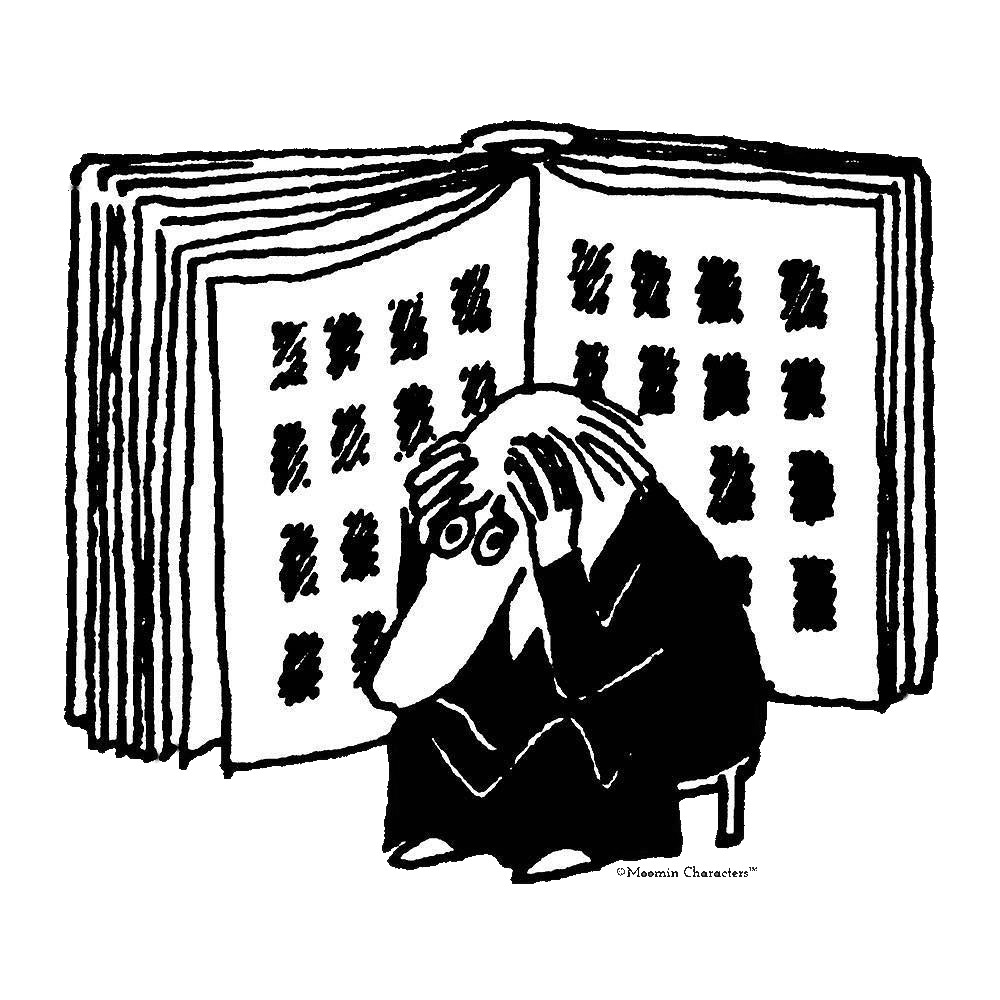
\includegraphics[width=240pt,height=240pt]{_6.jpg}
\caption{}
\label{_6}
\end{figure}

``Mi pensas ke mi komencas kompreni,'' diris Mumintrolo malrapide. ``Vi ne plu estas kolektanto, nur posedanto, kaj tio tute ne estas same amuza.''

``Ne,'' murmuris la hemulo korpremite. ``Tute ne.'' Li haltis kaj turnis sian sulkitan vizaĝon al ili.

``Kara hemulo,'' diris Snorkfraŭlino kaj delikate glatumis al li la manon.

``Mi havas ideon. Imagu se vi komencus kolekti ion tute alian, ion tute novan?''

``Jen ideo,'' konsentis la hemulo. Sed li ankoraŭ restis ĉifita, ĉar li pensis ke ne eblas ĝoji tuj post tiel granda ĉagreno.

``Ekzemple papiliojn?'' proponis Mumintrolo.

``Neeble,'' diris la hemulo kaj malgajiĝis. ``Tion kolektas mia kuzo je la patra flanko. Kaj mi ne eltenas lin.''

``Ĉu silkajn rubandojn?'' diris Snorkfraŭlino.

La hemulo nur elsnufis.

``Juvelojn?'' daŭrigis Snorkfraŭlino esperplene. ``Ili neniam elĉerpiĝas!''

``Aĉ!'' diris la hemulo.

``Nu, do ni vere ne scias,'' diris Snorkfraŭlino.

``Ni elpensos ion por vi,'' diris Mumintrolo konsole. ''Panjo certe scias.

Se paroli pri alio, ĉu vi jam vidis la moskoraton?''

``Li ankoraŭ dormas,'' respondis la hemulo malgaje. ``Li diris ke estas nenecese ellitiĝi tiel frue, kaj pri tio li vere pravis.'' Kaj la hemulo daŭrigis sian solecan vagadon tra la arbaro.

Mumintrolo kaj Snorkfraŭlino stiris siajn nubojn ĝis super la arbopintoj kaj malrapide balanciĝis antaŭen en la sunbrilo. Ili pensis pri io kion la hemulo povus kolekti.

``Ĉu konkojn?'' proponis Snorkfraŭlino.

``Aŭ pantalonbutonojn,'' diris Mumintrolo.

Sed la varmo dormemigis ilin. Ne eblis pensi. Ili kuŝiĝis surdorsen sur siaj nuboj kaj rigardis supren en la printempan ĉielon kie kantis alaŭdoj.

Kaj subite ili ekvidis la unuan papilion. Ĉiuj ja scias ke se la unua vidata papilio estas flava, tio signifas ke estos plezura somero. Se ĝi estas blanka nur estos trankvila somero (pri nigraj kaj brunaj papilioj ni entute ne parolu, tio estus ege tro malĝojiga).

Sed ĉi tiu papilio estis ora.

``Kion tio povas signifi?'' scivolis Mumintrolo. ``Oran papilion mi neniam antaŭe vidis.''

``Oro estas eĉ pli bona ol flavo,'' diris Snorkfraŭlino. ``Vi spertos!''

\begin{figure}[htbp]
\centering
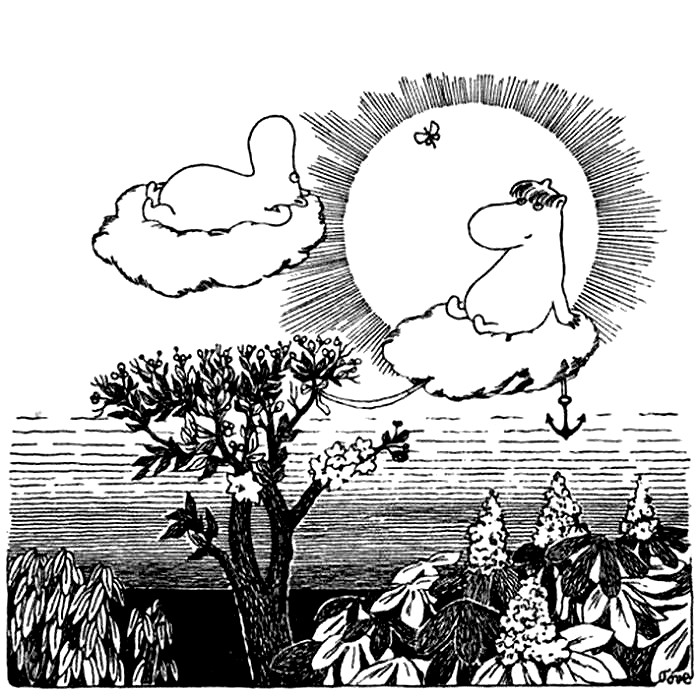
\includegraphics[width=400pt,height=400pt]{_7.jpg}
\caption{}
\label{_7}
\end{figure}

Kiam Mumintrolo kaj Snorkfraŭlino venis hejmen por la tagmanĝo la hemulo renkontis ilin sur la ŝtuparo. Li radiis pro ĝojo.

``Nu?'' diris Mumintrolo. ``Kio estos?''

``Plantoj!'' kriis la hemulo. ``Mi botanikos! La snorko elpensis tion. Mi kolektos la plej belan herbarion de la mondo!'' Kaj la hemulo etendis la jupon\footnote{La hemulo ĉiam estis vestita per robo kiun li heredis de sia onklino. Mi suspektas ke ĉiuj hemuloj portas jupon. Estas strange, sed tiel estas.

-- \emph{Noto de la aŭtoro.}} por montri al ili sian unuan trovaĵon. Inter tero kaj folioj kuŝis eta maldika orstelo.

``\emph{Gagea lutea},'' diris la hemulo fiere. ``Numero unu en la kolekto. Senerara ekzemplero.''

Kaj li eniris kaj ŝutis ĉion sur la manĝotablon.

``Movu tion al la angulo,'' diris Muminpatrino, ``ĉar ĉi tie la supo staros. Ĉu ĉiuj envenis? Ĉu la moskorato ankoraŭ dormas?''

``Kiel porko,'' diris Snif.

``Ĉu vi hodiaŭ amuziĝis?'' demandis Muminpatrino post kiam ŝi plenigis ĉiujn telerojn.

``Ege!'' kriis la tuta familio.
\sectionbreak
En la sekva mateno, kiam Mumintrolo iris al la ŝtipobudo por ellasi la kvin nubojn, ili jam malaperis, ĉiu el ili. Kaj neniu povis pensi ke tio iel rilatas al kelkaj ovoŝeloj kiuj denove kuŝas surfunde de la ĉapelo de sorĉisto.

\chapter[Dua Ĉapitro]{}


\begin{figure}[htbp]
\centering
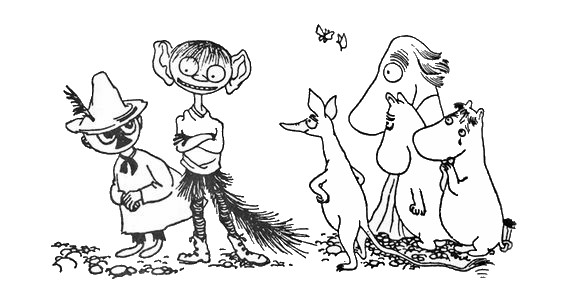
\includegraphics[width=450pt,height=243pt]{_8.jpg}
\caption{}
\label{_8}
\end{figure}

\begin{center}\textbf{\Large\color{ForestGreen}\textsc{Dua Ĉapitro}}\end{center}

\noindent\textit{en kiu oni rakontas kiel Mumintrolo transformiĝis en fantom-simion kaj finfine venĝis al la formikleono\footnote{Se vi ne scias, formikleono estas ruza insekto kiu fosis sin en la sablon, postlasanta malgrandan rondan truon super li. En ĉi tiun truon, nesupozaj etaj bestoj falas kaj tiam kapitas de la formikleono, kiu eliras el la fundo de la truo kaj formanĝas ilin.\\
Vi povas legi ĉion pri ĝi en la enciklopedio se vi ne kredas al mi. \emph{--- Tradukista noto}}, kaj krome pri la sekreta nokta vagado de Mumintrolo kaj Snufmumriko.}
\hfill \break
\hypertarget{Dua Ĉapitro}{}
\label{Dua Ĉapitro}


\noindent En iu varma kaj kvieta tago kiam somera pluvo falis sur Muminvalon oni decidis kaŝludi endome. Snif staris en unu angulo kun la vizaĝo enmane kalkulante laŭte. Kiam li venis ĝis dek li turnis sin kaj komencis serĉi; unue en la kutimaj kaŝejoj kaj poste en la strangaj.

Mumintrolo kuŝis sub la veranda tablo kaj sentis sin iomete maltrankvila. Ĝi ne \emph{estis} bona loko, tion li sentis. Snif certe levos la tablotukon, kaj tiam li estos kaptita. Mumintrolo rigardis tien-reen,

kaj tiam li ekvidis la nigran cilindran ĉapelon kiun iu metis en angulon. Tio estis brila ideo! Snif neniam ekpensos levi la ĉapelon. Mumintrolo rapide kaj silente rampis en la angulon kaj ŝovis la ĉapelon super la kapon. Ĝi ne atingis pli ol ĝis la ventro, sed se li tre malgrandigis sin kaj enŝovis la voston li certe estos sufiĉe nevidebla.

Mumintrolo subridis en sia soleco aŭdante ke ĉiuj aliaj estas trovataj, unu post la alia. La hemulo evidente refoje kaŝis sin sub la sofo -- li neniam trovis pli bonan lokon. Nun ili ĉiuj kuradis serĉante Mumintrolon.

Li atendis ĝis li komencis timi ke ili laciĝos serĉi, tiam li elrampis el la ĉapelo kaj enigis la kapon tra la pordo dirante: ``Ku ku!''

Snif longe gapis al li, poste li diris sufiĉe malamike: ``Ku ku al vi mem!''

``Kiu estas tiu?'' flustris Snorkfraŭlino.

La aliaj skuis la kapojn kaj gapis plu al Mumintrolo.

Kompatinda Mumintroleto! En la ĉapelo de sorĉisto li transformiĝis en tre strangan beston. Ĉio kio estis ronda ĉe li nun iĝis malvasta, kaj ĉio malgranda grandiĝis. Kaj plej strange el ĉio estis ke li mem sola ne povis vidi kio okazis.

``Jen vi sendube surpriziĝis,'' diris Mumintrolo kaj faris malcertan paŝon antaŭen per siaj altaj, malstabilaj kruroj. ``Vi tute ne scias kie mi estis!''

``Tio ne interesas nin,'' diris la snorko. ``Sed vi efektive aspektas tiel malbele ke ĉiu ajn povus surpriziĝi.''

``Kiel malamikaj vi estas,'' murmuris Mumintrolo malgaje. ``Eble vi devis tro longe serĉi. Kion ni nun faru?''

``Unue vi eble devus prezenti vin,'' diris Snorkfraŭlino rigide. ``Ni ja tute ne scias kiu vi estas.''

Mumintrolo surprizite rigardis ŝin, sed poste li ekpensis ke ĉi tio estas nova ludo. Li gaje ridis kaj diris: ``Mi estas la Reĝo de Kalifornio!''

``Kaj mi estas la snorka fratino,'' diris Snorkfraŭlino. ``Ĉi tiu estas mia frato.''

``Mi nomiĝas Snif,'' diris Snif.

``Mi estas Snufmumriko,'' diris Snufmumriko.

``Aĉ, kiel tedaj vi estas,'' diris Mumintrolo. ``Ĉu vi ne povus elpensi ion pli malkutiman! Nun ni iru eksteren, mi pensas ke baldaŭ sereniĝos.'' Li iris eksteren sur la ŝtuparon, kaj la aliaj sekvis lin, tre surprizite kaj sufiĉe suspekteme.

``Kiu estas li?'' demandis la hemulo kiu sidis ekster la domo kalkulante stamenojn en sunfloro.

``Li estas la Reĝo de Kalifornio,'' diris Snorkfraŭlino hezite.

``Ĉu li loĝos ĉi tie?'' demandis la hemulo.

``Tion Mumintrolo decidos,'' diris Snif. ``Mi vere scivolas kien li malaperis.''

Mumintrolo ridis. ``Vi vere kelkfoje estas sufiĉe amuza,'' li diris. ``Imagu, se ni serĉadus Mumintrolon!''

``Ĉu vi konas lin?'' demandis Snufmumriko.

``Nu,'' diris Mumintrolo. ``Eblus diri ke jes! Sufiĉe bone, efektive!'' Li estis preta krevi pro feliĉo pri la nova ludo kaj pensis ke li mastras ĝin bonege.

``Kiam vi ekkonis lin?'' demandis Snorkfraŭlino.

``Ni naskiĝis samtempe,'' respondis Mumintrolo kaj preskaŭ eksplodis pro amuziĝo. ``Sed vi sciu, li estas vere fieraĉa! Apenaŭ eblas akcepti lin en normala kompanio!''

``Fi, tiel vi ne rajtas diri pri Mumintrolo,'' diris Snorkfraŭlino bruske. ``Li estas la plej bona trolo de la mondo kaj ni treege ŝatas lin!''

Mumintrolo estis ravita. ``Ĉu vere?'' li diris. ''Miaflanke mi trovas Mumintrolon vera pestulo.

Tiam Snorkfraŭlino ekploris.

``Foriru,'' diris la snorko minace. ``Alie ni batos vin!''

``Nu nu,'' diris Mumintrolo konsternite. ``Tio ja estis nura ludo! Mi tre ĝojas ke vi tiom ŝatas min.''

``Ni \emph{tute} ne ŝatas vin!'' kriis Snif akre. ``Ek kontraŭ li! Forpelu la aĉan reĝon kiu diras malbelaĵojn pri nia mumintrolo!''

Kaj ili kune ĵetis sin kontraŭ la kompatinda Mumintrolo. Li estis ege tro konsternita por povi defendi sin, kaj kiam li havis tempon koleri, jam estis tro malfrue; li kuŝis plej sube en pugnanta kaj krianta pelmelo el brakoj, vostoj kaj kruroj. Muminpatrino elvenis sur la ŝtuparon.

``Kio okazas al vi, idoj!'' ŝi vokis. ``Tuj ĉesu batali!''

``Ili batas la reĝon de Kalifornio!'' singultis Snorkfraŭlino. ``Kaj ili pravas!''

Mumintrolo krablis antaŭen, laca kaj kolera.

``Panjo!'' li kriis. ``Ili komencis! Tri kontraŭ unu, tio ne estas justa!''

``Mi konsentas pri tio,'' diris Muminpatrino serioze. ``Sed vi certe incitis ilin. Cetere, kiu vi estas, besteto?''

``Ĉesigu tiun stultan ludon,'' kriis Mumintrolo. ``Vi tute ne estas amuzaj. Mi estas Mumintrolo, kaj jen staras mia panjo sur la ŝtuparo. Punkto, fino!''

``\emph{Vi} ne estas Mumintrolo,'' diris Snorkfraŭlino malestime. ``Li havas etajn belajn orelojn, sed viaj aspektas kiel pottukoj!''

Mumintrolo konfuzite palpis sian kapon kaj ekkaptis paron da terure grandaj, ĉifitaj oreloj. ``Sed mi \emph{estas} Mumintrolo!'' li ekkriis senespere. ``Ĉu vi ne kredas min?''

``Mumintrolo havas konvene malgrandan voston, sed la via aspektas kiel lampobroso,'' diris la snorko.

Ho, estis vere! Mumintrolo palpis postaĵe per tremantaj manoj.

``Viaj okuloj similas telerojn,'' diris Snif. ``Tiujn de Mumintrolo estis etaj kaj amikaj!''

``Prave,'' konfirmis Snufmumriko.

``Vi estas trompulo!'' decidis la hemulo.

``Ĉu neniu kredas min?'' ekkriis Mumintrolo. ``Zorge rigardu min, Panjo, kaj vi devas rekoni vian muminidon!''

Muminpatrino zorge observis. Ŝi rigardis en liajn timigitajn telerajn okulojn, tre longe, kaj poste ŝi diris kviete: ``Jes, vi estas Mumintrolo.''

Kaj ĝuste en tiu momento li komencis transformiĝi. La okuloj, oreloj kaj vosto ŝrumpis, la nazo kaj ventro kreskis. Kaj jen staris Mumintrolo kompleta antaŭ ili en plena majesto.

``Venu en miajn brakojn,'' diris Muminpanjo. ``Vidu, mian etan muminidon mi tamen ĉiam rekonos.''
\sectionbreak
Pli malfrue en tiu tago Mumintrolo kaj la snorko sidis en unu el la sekretaj lokoj, tiu sub la jasmeno, kie oni estas ĉirkaŭata de de verda ronda folia groto.

``Jes, sed ja \emph{devas} esti iu kiu transformis vin'', diris la snorko.

Mumintrolo kapneis. ``Mi vidis nenion mirindan,'' li diris. ``Kaj mi nenion manĝis, nek diris danĝerajn vortojn.''

``Sed vi eble hazarde eniris sorĉan ringon,'' cerbumis la snorko.

``Ne laŭ mia scio,'' diris Mumintrolo. ``La tutan tempon mi sidis sub la nigra ĉapelo kiun ni uzas kiel paperkorbon.''

``Ene de la \emph{ĉapelo}?'' demandis la snorko nekredeme.

``Ĝuste tie,'' diris Mumintrolo. Ili cerbumis ankoraŭ iom. Poste ili ekkriis samtempe: ``Devas esti{\ldots}!'' gapante unu al la alia.

``Venu!'' diris la snorko.
\sectionbreak
Ili supreniris en la verandon kaj proksimiĝis al la ĉapelo, tre singarde.

``Ĝi ŝajnas sufiĉe ordinara,'' diris la snorko. ``Se oni ne konsideras ke cilindra ĉapelo ĉiam estas sufiĉe neordinara, kompreneble.''

``Sed kiel ni \emph{eksciu} ĉu estis tiu?'' scivolis Mumintrolo. ``\emph{Mi} ne eniros ĝin duafoje!''

``Eble oni povus logi iun alian tien,'' diris la snorko penseme.

``Sed tio estus sufiĉe malnobla,'' diris Mumintrolo. ``Kiel ni povas scii ke li refariĝos ĝusta?''

``Ni prenu malamikon,'' proponis la snorko.

``Hm,'' diris Mumintrolo. ``Ĉu vi konas iun?''

``La grandan raton sur la rubamaso,'' diris la snorko.

Mumintrolo kapneis. ``Ne eblas trompi ĝin.''

``Nu, do la formik-leonon?'' proponis la snorko.

``En ordo,'' diris Mumintrolo. ``Iufoje li trenis mian patrinon suben en kavon kaj ĵetis sablon en ŝiajn okulojn.''

Ili ekiris por trovi la formik-leonon kaj kunportis grandan skatolon. La ruzajn kavojn de la formikleono oni devas serĉi sur la sablostrando, do ili piediris ĝis la maro. Ne daŭris longe ĝis la snorko trovis grandan rondan kavon kaj fervore signalis al Mumintrolo.

``Jen li estas!'' flustris la snorko. ``Sed kiel ni logu lin en la skatolon?''

``Lasu min zorgi pri tio,'' flustris Mumintrolo al li. Poste li prenis la skatolon kaj kaŝis ĝin en la sablo iom for kun la buŝo supren. Poste Mumintrolo diris per laŭta voĉo: ``Ili estas sufiĉe malfortaj mizeruloj, tiuj formik-leonoj!'' Li faris signon al la snorko kaj ambaŭ esperplene rigardis suben en la kavon. La sablo moviĝis tie sube sed nenio vidiĝis.

``\emph{Tre} malfortaj!'' daŭrigis Mumintrolo. ``Ili bezonas \emph{plurajn horojn} por enfosi sin mem en la sablon, kredu min!''

''Jes, sed{\ldots} ''diris la snorko dubante.

``Certe,'' diris Mumintrolo farante furiozajn signojn per la oreloj. ``Plurajn horojn!''

Tiumomente minaca kapo kun gapantaj okuloj aperis el la sablokavo.

\begin{figure}[htbp]
\centering
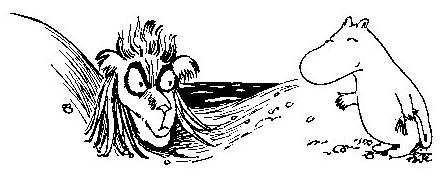
\includegraphics[width=400pt,height=161pt]{_9.jpg}
\caption{}
\label{_9}
\end{figure}

``Ĉu vi diris malforta?'' siblis la formikleono. ``Mi enfosas min en tri sekundoj, nek pli nek malpli!''

``Sinjoro, vi sendube devus montri al ni kiel tio okazas por ke ni kredu tion,'' diris Mumintrolo flate.

``Mi ĵetos sablon al vi,'' diris la formikleono kolere. ``Kaj ĵetinte vin en mian kavon mi manĝos vin!''

``Ne, ne,'' petis la snorko timeme. ``Prefere montru al ni kiel rampi malantaŭen en la sablon en tri sekundoj!''

``Faru tion ĉi-supre kie ni pli bone vidos kiel vi faras,'' diris Mumintrolo kaj montris al la loko kie la skatolo estis kaŝita.

``Ĉu vi pensas ke mi zorgas akrobati antaŭ infanetoj,'' diris la formikleono moke. Sed li ne povis rezisti la tenton montri al ili kiel rapida kaj forta li estas. Dum malestimaj elsnufoj li rampis supren el sia kavo kaj fieraĉe demandis: ``Nu, kie mi enfosu min?''

``Jen,'' diris Mumintrolo montrante.

La formikleono levis la ŝultrojn kaj starigis la kolharojn en timiga maniero.

``Atentu!'' li kriis. ``Nun mi iros subteren, sed revenante mi manĝos vin! Unu, du, tri!''

Kiel rotacianta helico la formikleono retroiris suben en la sablon, rekte en la skatolon kaŝitan sub li. Tio vere okazis en tri sekundoj, aŭ eble eĉ en du kaj duono, ĉar li estis tiel terure kolera.

``Rapide surmetu la kovrilon!'' kriis Mumintrolo. Ili forgratis la sablon kaj alŝraŭbis la kovrilon per granda forto. Poste ili per kuna peno levis la skatolon kaj komencis ruli ĝin hejmen. La formikleono kriis kaj plendegis ene, sed la sablo sufokis lian voĉon.

``Estas abomene kiel li koleras,'' diris la snorko. ``Mi ne kuraĝas pensi kio okazus se li elvenus!''

``Li ne elvenos,'' diris Mumintrolo trankvile. ``Kaj kiam li faros tion, mi esperas ke li estos transformita en ion teruran!''

Alveninte al la mumindomo Mumintrolo kolektis siajn amikojn ŝovante la manojn enbuŝen kaj farante tri longajn fajfojn (kio signifis: io neimagebla okazis).

La aliaj alkuris de ĉiuflanke kaj kolektiĝis ĉirkaŭ la skatolo kun ŝraŭbita kovrilo.

``Kion vi havas tie?'' demandis Snif.

``Formik-leonon,'' diris Mumintrolo fiere. ``Vera, kolera formikleono kiun ni kaptis!''

``Imagu, ke vi kuraĝis!'' ekkriis Snorkfraŭlino admire.

``Kaj nun ni intencas elŝuti lin en la ĉapelon,'' diris la snorko.

``Por ke li estu transformita en fantom-simion, kiel mi estis,'' diris Mumintrolo.

``Parolu normale tiel ke ni ion komprenos,'' petis la hemulo.

``Mi estis transformita pro tio ke mi kaŝis min en tiu ĉapelo,'' klarigis Mumintrolo. ``Ni elpensis tion. Kaj nun ni kontrolos la aferon esplorante ĉu ankaŭ la formikleono iĝos io alia.''

``Sed li ja povos iĝi io ajn!'' kriis Snif. ``Li povos iĝi io eĉ pli danĝera ol formikleono kaj formanĝi nin ĉiujn!'' Dum kelka tempo ili staris en tima silento rigardante la skatolon kaj aŭskultante la obtuzajn sonojn el ĝi.

``Oj, oj,'' diris Snorkfraŭlino time kaj perdis sian koloron\footnote{Snorkoj ofte ŝanĝas koloron je emocioj. --- \emph{Noto de la aŭtoro}}.

``Ni kaŝos nin subtable dum li transformiĝos kaj metos dikan libron sur la ĉapelo,'' proponis Snufmumriko. ``Oni ĉiam devas riski ion kiam oni eksperimentas! Nun tuj enŝutu lin!''

Snif rapidis kaŝiĝi subtable. Mumintrolo, Snufmumriko kaj la hemulo tenis la skatolon super la ĉapelo de sorĉisto, kaj Snorkfraŭlino timante deŝraŭbis la kovrilon. En nubo el sablo la formikleono falis en la ĉapelon, kaj fulmrapide la snorko metis vortaron kun fremdlandaj vortoj super ĉion. Poste ĉiuj kuris kaŝiĝi sub la tablo.

Unue nenio okazis.

Ili gvatis sub la tablotuko atendante en kreskanta maltrankvilo. Neniu ŝanĝo.

``Tio estis nura blago,'' diris Snif. Subite la vortaro kun fremdlandaj vortoj komencis ĉifiĝi. Snif mordis la dikfingron de la hemulo pro pura ekscitiĝo.

``Atentu,'' diris la hemulo kolere. ``Vi mordis mian dikfingron!''

``Ho, pardonu,'' diris Snif. ``Mi pensis ke ĝi estas mia!''

Nun la vortaro pli kaj pli kunvolviĝis. La paĝoj komencis simili velkintajn arbofoliojn. Kaj inter ili ĉiuj fremdlandaj vortoj elrampis kaj komencis krabladi tien-reen surplanke.

``Kia strangaĵo!'' diris Mumintrolo.

Sed nun denove io okazis. Komencis guti de la ĉapelaj randoj. Fluis.

Riveroj el akvo plaŭdis suben sur la tapiŝon tiel ke la fremdlandaj vortoj devis savi sin supren laŭ la muroj.

``La formikleono iĝis nura akvo,'' diris Snufmumriko elrevigite.

``Mi pensas ke tio estas la sablo,'' flustris la snorko. ``La formikleono sendube venos post kelka tempo.''

\begin{figure}[htbp]
\centering
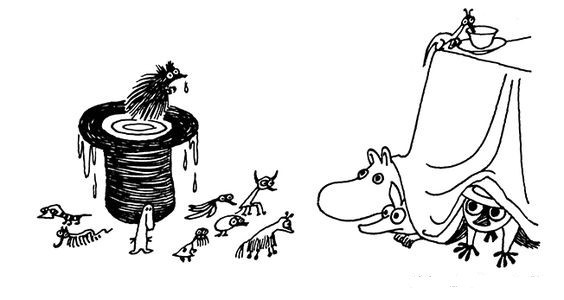
\includegraphics[width=450pt,height=239pt]{_10.jpg}
\caption{}
\label{_10}
\end{figure}

Denove ili atendis en neeltenebla ekscito. Snorkfraŭlino kaŝiĝis en la brakoj de Mumintrolo kaj Snif pepis pro timego. Tiam subite montris sin sur la ĉapelrando la plej malgranda erinaco de la mondo. Ĝi flaris aeren kaj palpebrumis, kaj ĝi estis tute taŭzita kaj malseka.

Dum kelkaj sekundoj regis tomba silento. Poste Snufmumriko komencis ridi. Kaj la aliaj daŭrigis kiam li devis ripozi. Ili hurlis pro rido kaj ruliĝis subtable pro pura plezuro. Nur la hemulo ne dividis la amuziĝon. Li surprizite rigardis siajn amikojn kaj diris: ``Bone, sed ni ja atendis ke la formikleono estos transformita! Se mi povus kompreni kial vi ĉiam tiom bruas pri aferoj.''

Dume la eta erinaco solene kaj iom malĝoje paŝis ĝis la pordo kaj iris suben laŭ la ŝtupoj. La akvo ĉesis flui kaj plenigis la verandan plankon kiel lago. Kaj la tuta plafono estis plena de fremdlandaj vortoj.
\sectionbreak
Kiam oni klarigis ĉion al la gepatroj de Mumintrolo, ili prenis la aferon tre serioze kaj decidis ke la ĉapelo de sorĉisto estos detruita. Oni singarde rulis ĝin en la riveron kaj lasis ĝin fali en la akvon.

``Do, \emph{tio} estis la nuboj kaj la fantom-simio,'' diris la patrino de Mumintrolo, dum ili rigardis la forflosantan ĉapelon.

``Ili estis amuzaj nuboj,'' diris Mumintrolo iom mishumore. ``Povus aperi pliaj!''

``Aŭ riveregoj kaj fremdaj vortoj, jes ja,'' diris lia patrino. ``Kiel aspektis en la verando! Kaj mi ne povas imagi kiel mi liberiĝos de tiuj bestetoj. Ili ĉie ĝenas kaj kaŭzas malordon en la tuta domo!''

``Tamen la nuboj \emph{estis} amuzaj,'' insiste murmuris Mumintrolo.

Vespere Mumintrolo ne povis endormiĝi. Li kuŝis rigardante eksteren en la helan junian nokton plenan de solecaj vokoj, plandado kaj dancado. Bonodoris de floroj.

Snufmumriko ankoraŭ ne revenis hejmen. Ĉi tiajn noktojn li ofte vagadis sola kun si mem kaj sia buŝharmoniko. Sed ĉi-nokte aŭdiĝis neniuj kantoj. Li sendube faris esplorvagadon. Baldaŭ li starigos sian tendon ĉe la riverbordo kaj rifuzos dormi endome{\ldots} Mumintrolo suspiris. Li sentis sin malĝoja kvankam li havis nenion pri kio malĝoji.

Ĝuste tiam aŭdiĝis mallaŭta fajfo sub la fenestro. La koro de Mumintrolo saltis pro ĝojo kaj li malrapide ŝteliris ĝis la fenestro por rigardi eksteren. La fajfo signifis: Sekretoj! Snufmumriko atendis sub la ŝnura ŝtupetaro.

``Ĉu vi povas konservi sekreton?'' li flustris kiam Mumintrolo tretis sur la herbojn.

Mumintrolo fervore kapjesis. Snufmumriko klinis sin antaŭen kaj flustris eĉ pli mallaŭte: ``La ĉapelo drivis alborden sur sablobenko iom pli malsupre laŭ la rivero.''

La okuloj de Mumintrolo eklumis.

``Ĉu vi volas?'' demandis Snufmumriko per la brovoj.

``Certe!'' respondis Mumintrolo per eta orelsvingo.

Kiel ombroj ili ŝteliris tra la rosoplena ĝardeno al la rivero.

``Ĝi kuŝas je du riverkurbiĝoj for de ĉi tie,'' diris Snufmumriko nelaŭte. ``Efektive ni ŝuldas savi ĝin, ĉar la akvo kiu plenigas ĝin ruĝiĝas. La loĝantoj pli malsupre laŭ la rivero estos teruritaj de tiu timiga akvo.''

``Ni devus pensi pri tio,'' diris Mumintrolo. Li sentis sin fiera kaj ĝoja paŝi ĉi tiel kun Snufmumriko meze de la nokto. Antaŭe Snufmumriko ĉiam estis sola en sia nokta vagado.

``Jen ie ĝi estas,'' diris Snufmumriko. ``Kie komenciĝas la malhela strio en la akvo. Ĉu vi vidas?''

``Ne vere,'' diris Mumintrolo kiu stumblis antaŭen tra la duonmallumo. ``Mi ne havas noktajn okulojn kiel vi.''

``Mi demandas min kiel kapti ĝin,'' pripensis Snufmumriko kiu rigardis al la rivero. ``Kiel stulte ke via patro ne havas boaton.''

Mumintrolo hezitis. ``Mi naĝas sufiĉe bone se la akvo ne estas tro malvarma, li diris.''

``Vi ne kuraĝas,'' diris Snufmumriko dubante.

``Certe mi kuraĝas,'' diris Mumintrolo kaj tuj sciis ke li faros tion. ``En kiu direkto ĝi estas?''

``Oblikve tien,'' diris Snufmumriko. ``Vi baldaŭ atingos la fundon sur la sablobenko. Sed atentu ne ŝovi la manojn en la ĉapelon. Tenu la ĉapelverton.''

Mumintrolo englitis en la somere varman akvon kaj hunde naĝis en la riveron. Tie estis forta fluo, kaj certatempe li iom maltrankvilis. Nun li vidis la sablobenkon kaj sur ĝi ion nigran. Li stiris pli proksimen per la vosto kaj baldaŭ sentis sablon sub la piedoj.

\begin{figure}[htbp]
\centering
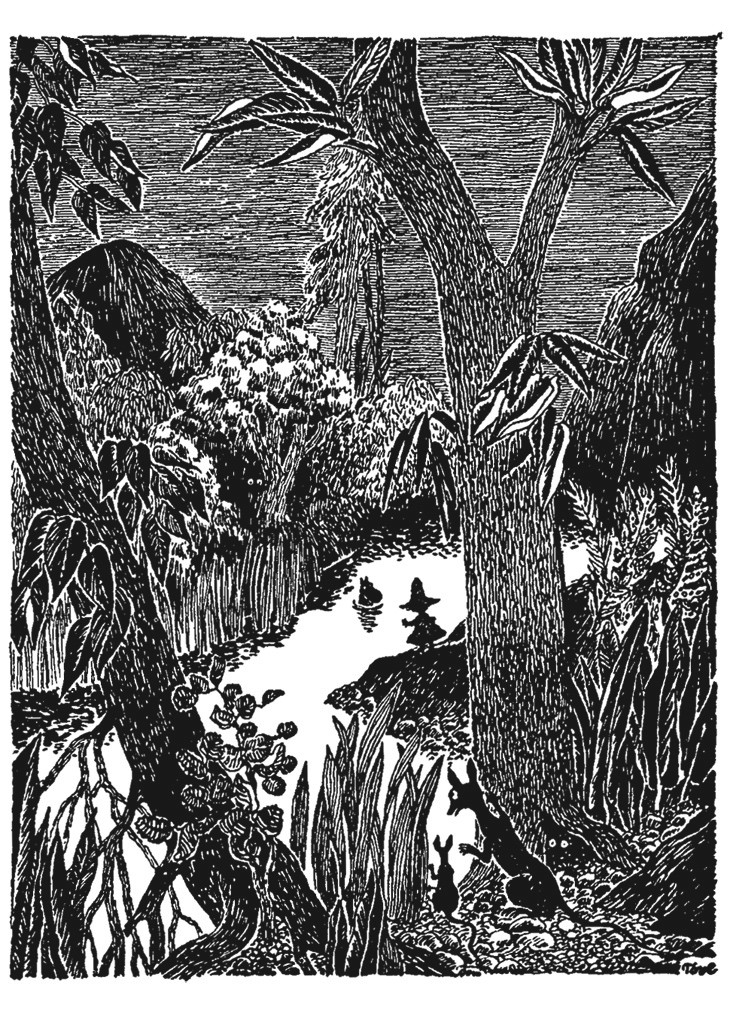
\includegraphics[width=450pt,height=631pt]{_11.jpg}
\caption{}
\label{_11}
\end{figure}

``Ĉu ĉio en ordo?'' vokis Snufmumriko mallaŭte de la bordo.

``Ĉio en ordo!'' respondis Mumintrolo kaj vadis supren sur la sablorifon.

Li vidis malhelan fluon serpenti el la ĉapelo malsupren en la rivero. Tio estis la ruĝa transformita akvo. Mumintrolo ŝovis manon en la akvon kaj hezite lekis ĝin.

``Kia strangaĵo!'' li murmuris. ``--- Tio ja estas fruktsuko! Imagu, de nun ni povos ricevi kiom ajn da suko ni deziras nur verŝante akvon en la ĉapelon!''

``Nu, ĉu vi havas ĝin?'' vokis Snufmumriko maltrankvile.

``Mi venos!'' respondis Mumintrolo kaj vadis reen en la akvon kun la vosto firme nodita ĉirkaŭ la ĉapelo de sorĉisto. Estis malfacile naĝi kontraŭ la fluo kun la peza ĉapelo trenata poste, kaj kiam Mumintrolo rampis sur la strandon li estis terure laca.

``Jen ĝi,'' li fiere spiregis.

``Bone,'' diris Snufmumriko. ``Sed kien ni metu ĝin?''

``Ne en la mumindomon,'' diris Mumintrolo. ``Prefere ne en la ĝardenon. Iu povus trovi ĝin.''

``Kion vi opinias pri la groto?'' cerbumis Snufmumriko.

``Tiam ni devos dividi la sekreton kun Snif,'' diris Mumintrolo. ``Estas lia groto.''

``Do ni devos fari tion,'' diris Snufmumriko hezite. ``Sed li estas sufiĉe malgranda por koni tiel grandan sekreton.''

``Jes,'' diris Mumintrolo serioze. ``Sciu, ĉi tio estas la unua fojo kiam mi faras ion kion mi ne povas rakonti al Paĉjo kaj Panjo.''

Snufmumriko prenis la ĉapelon en la brakoj kaj ekiris reen laŭ la rivero. Kiam ili atingis la ponton Snufmumriko subite haltis.

``Kio estas?'' flustris Mumintrolo maltrankvile.

``Kanarioj!'' ekkriis Snufmumriko. ``Tri flavaj kanarioj jen sur la ponta apogilo. Strange vidi ilin eksterdome dumnokte.''

``Mi tute ne estas ia kanario,'' pepis la plej proksima birdo. ``Mi estas ploto!''

``Ni ĉiuj tri estas honestaj fiŝoj!'' trilis lia kamarado.

Snufmumriko skuis la kapon.

``Jen vi vidas kion la ĉapelo kaŭzas,'' li diris. ``Tiuj tri fiŝetoj certe naĝis en ĝin kaj estis transformitaj. Venu, ni iru rekte ĝis la groto por kaŝi la ĉapelon!''

Mumintrolo tenis sin proksime post Snufmumriko dum ili trairis la arbaron. Ĉiuflanke io susuris kaj plandis, kaj li trovis tion preskaŭ iomete terura. Jen lumantaj okuletoj gapis al ili de malantaŭ arbotrunkoj, jen iu vokis al ili de la tero aŭ arbopintoj.

``Belan nokton!'' Mumintrolo aŭdis voĉon rekte malantaŭ si.

``Belan!'' li kuraĝe respondis. Kaj eta ombro preterglitis lin en la mallumon.

Surstrande estis pli hele. Maro kaj ĉielo kunfandiĝis en unu palbluan, gliman surfacon. De malproksime aŭdiĝis solaj alvokoj de birdoj. Jam estis proksime al la mateno. Snufmumriko kaj Mumintrolo portis la ĉapelon de sorĉisto supren en la groton kaj metis ĝin renversite en la plej internan angulon por ke nenio povu fali en ĝin.

``Ĉi tio sendube estas la plej bona kion ni povus fari,'' diris Snufmumriko. ``Kaj imagu, se ni povus rericevi la kvin nubetojn!''

``Jes!'' diris Mumintrolo kiu staris en la groto-buŝo rigardante eksteren en la nokton. ``Sed mi demandas min ĉu ili povus plibeligi tion kio estas ĝuste nun{\ldots}''

\chapter[Tria Ĉapitro]{}


\begin{figure}[htbp]
\centering
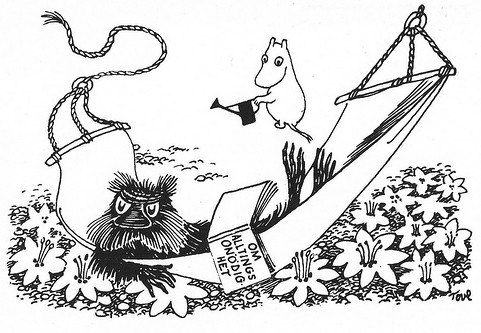
\includegraphics[width=450pt,height=310pt]{_12.jpg}
\caption{}
\label{_12}
\end{figure}

\begin{center}\textbf{\Large\color{ForestGreen}\textsc{Tria Ĉapitro}}\end{center}

\noindent\textit{en kiu oni priskribas kiel la moskorato retiriĝis en dezerton kaj spertis ion nedireblan, kiel Aventuro portis la muminfamilion ĝis la soleca insulo de hatifnatoj kie la hemulo preskaŭ forbrulis kaj kiel la granda fulmotondro pasis super ili.}
\hfill \break
\hypertarget{Tria Ĉapitro}{}
\label{Tria Ĉapitro}


\noindent En la sekva mateno kiam la moskorato kiel kutime eliris eksterdomen kun sia libro kaj kuŝiĝis en la hamakon por legi pri la neneceso de ĉio, la ŝnuro rompiĝis kaj li falis teren.

``Nedefendeble!'' diris la moskorato kaj liberigis sin de la plejdo.

``Domaĝe!'' diris la patro de Mumintrolo kiu akvumis siajn tabakplantojn. ``Mi esperas ke vi ne vundiĝis?''

``Ne temas pri \emph{tio},'' diris la moskorato malgaje tirante siajn lipharojn. ``La tero povas fendiĝi se ĝi volas, tio ne ŝancelus mian trankvilon. Sed mi ne ŝatas esti metita en ridindajn situaciojn. Tio estas maldigna!''

``Sed \emph{mi} estis la sola kiu vidis vin,'' kontraŭis Muminpatro.

``Bedaŭrinde!'' diris la moskorato. ``Ne estas malmulte kion mi suferis en via domo. Lastjare, ekzemple, kometo falis sur min. Tio ne gravis. Sed kiel vi eble memoras, mi sidiĝis sur la ĉokoladan kukon de via edzino! Tio estis ekstreme embarasa por mia digno! Mi trovas harbrosojn en mia lito -- treege stulta ŝerco. Se ne paroli pri{\ldots}''

``Mi scias, mi scias,'' interrompis la patro korpremite. ``Sed ĉi tio ne estas kvieta domo. Kaj ŝnuroj kelkfoje maldikiĝas kun la paso de jaroj{\ldots}''

``Ili ne \emph{rajtas},'' diris la moskorato. ``Kompreneble ne gravus se mi mortbatiĝus. Sed imagu se la ALIAJ rigardus! Nun mi tamen intencas retiriĝi en la dezerton por vivi vivon en soleco kaj kvieto kaj rezigni ĉion. Jen mia firma decido.''

``Ĉu vere?'' diris la patro de Mumintrolo admire. ``Kie do?''

``En la groto,'' diris la moskorato. ``Tie nenio povos ĝeni miajn pensojn per stultaj ŝercoj. Vi povos alporti manĝon al mi dufoje tage. Sed ne antaŭ la deka horo.''

``Bone,'' diris la patro humile. ``Ĉu ni portu meblojn tien?''

``Vi povas fari tion,'' diris la moskorato iom pli amike. ''Sed tre simplajn.

Mi komprenas ke vi ne malbonvolas, sed via familio pelis min ĝis la limo de mia pacienco.'' Poste la moskorato prenis sian libron kaj sian plejdon kaj malrapide marŝis supren laŭ la deklivo. Muminpatro dum kelka tempo suspiris en soleco, poste li plu akvumis la tabakon kaj baldaŭ forgesis la tuton.

Kiam la moskorato venis en la groton li sentis sin tre kontenta. Li sternis la plejdon sur la sablan grundon, sidiĝis sur ĝin kaj tuj komencis pensi. Li plu faris tion dum proksimume du horoj. Ĉio estis silenta kaj paca, kaj tra la fendego en la grota plafono la suno milde brilis al lia soleca rifuĝejo. De temp' al tempo la moskorato iom moviĝis kiam la sunstrio formigris de li.

\begin{figure}[htbp]
\centering
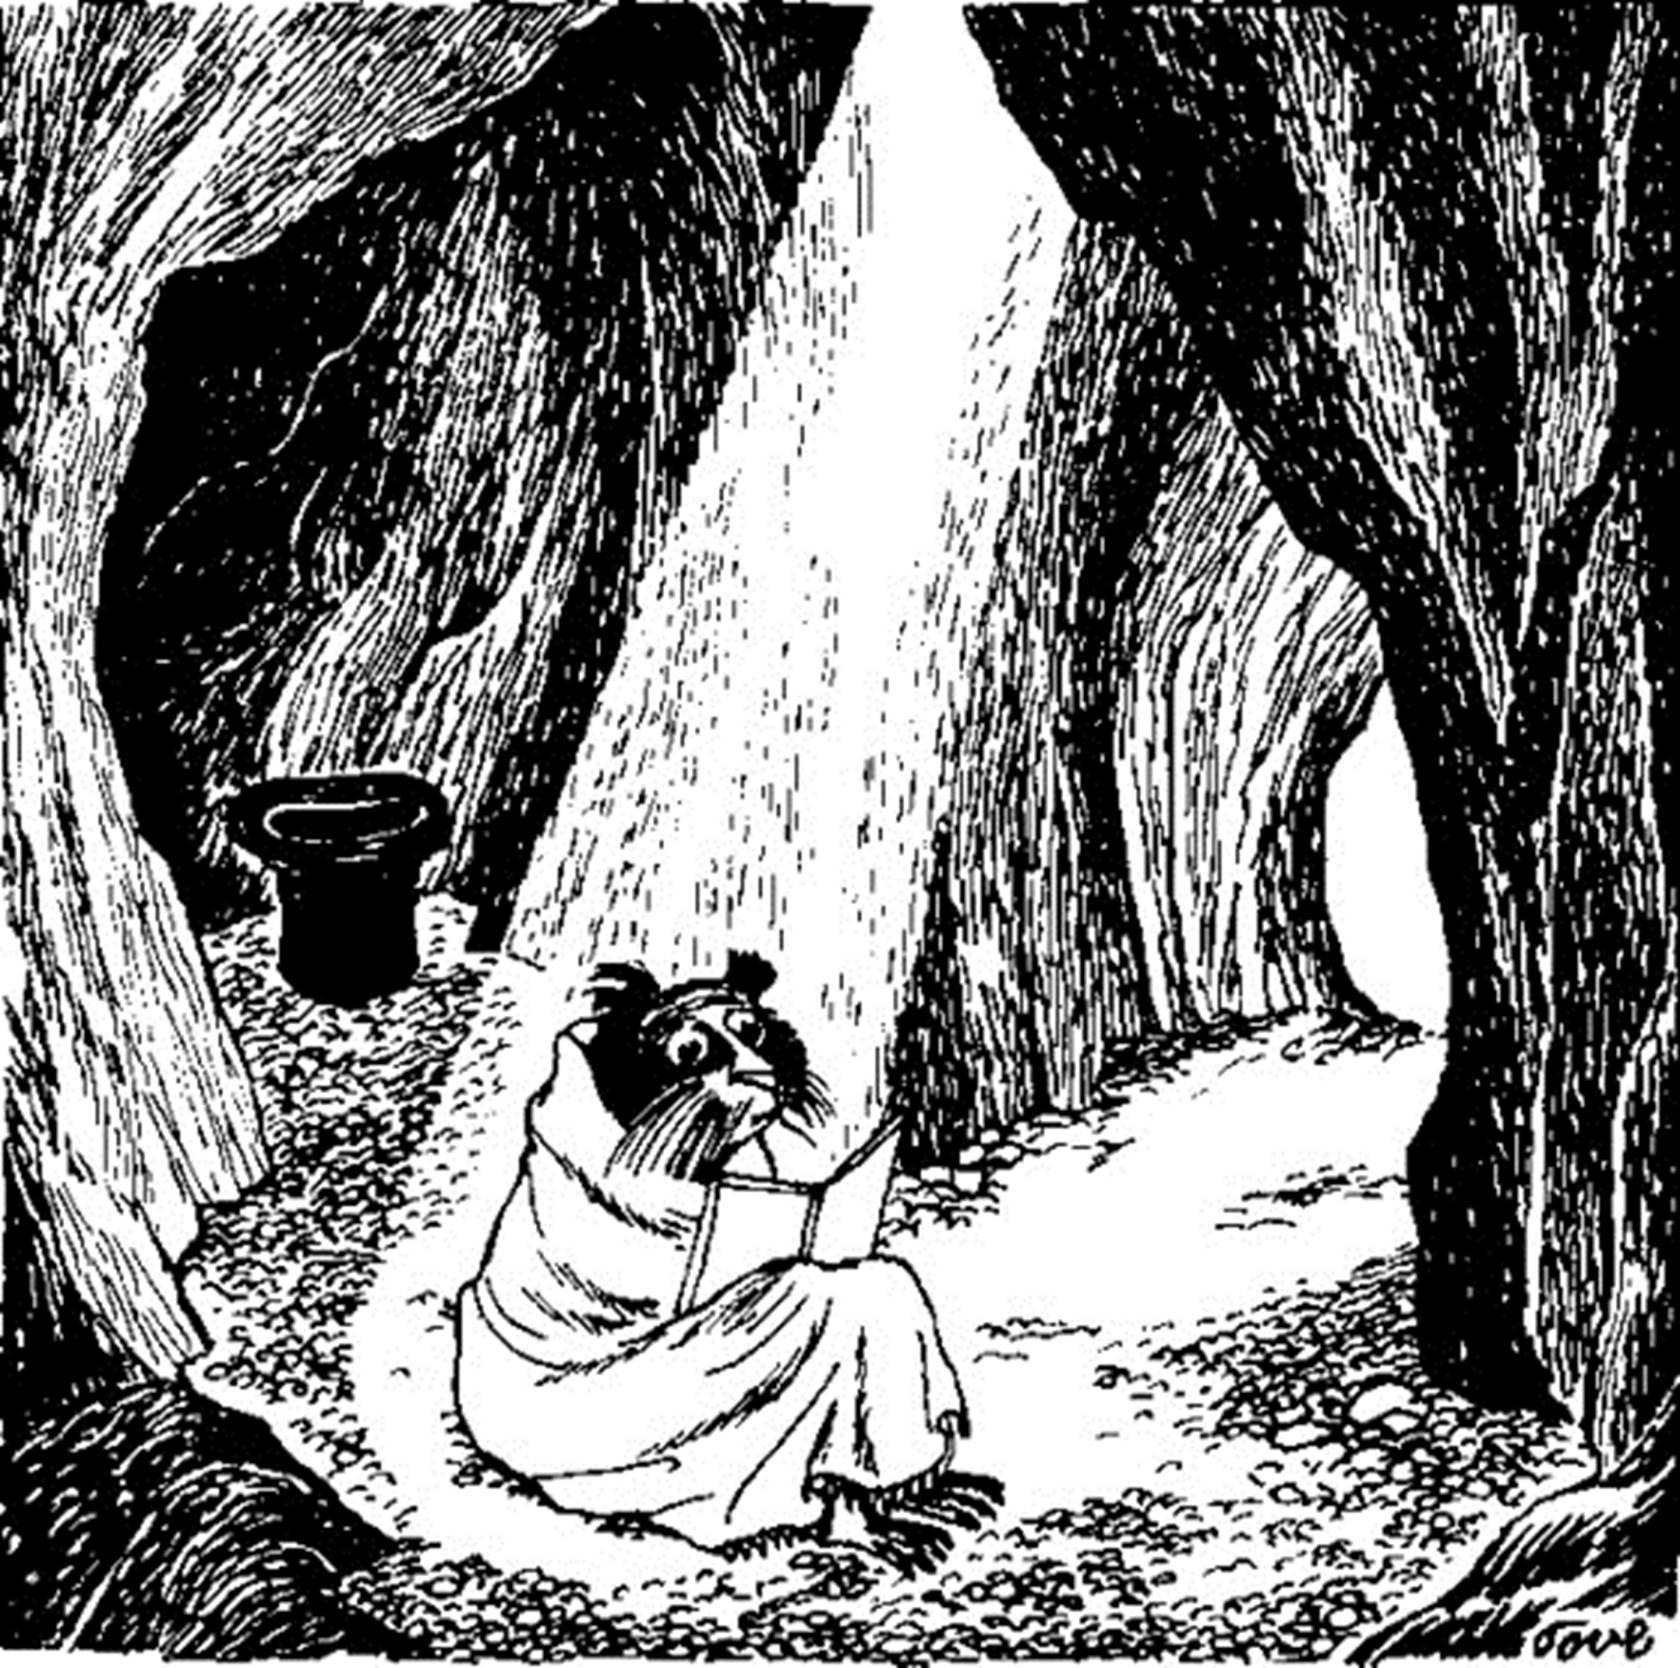
\includegraphics[width=459pt,height=455pt]{_13.jpg}
\caption{}
\label{_13}
\end{figure}

`Ĉi tie mi restos ĉiame, ĉiame,' li pensis. `Ĉu ne estas nenecese saltadi kaj babili, konstrui domojn kaj kuiri manĝon kaj kolekti posedaĵojn?'

Kontente li rigardis ĉirkaŭ si en sia nova hejmo, kaj tiam li ekvidis la ĉapelon de sorĉisto, kiun Mumintrolo kaj Snufmumriko kaŝis en la plej fora angulo.

``La paperkorbo,'' diris la moskorato al si. ``Do, ĉu ĝi staras ĉi tie? Nu, ĝi sendube utilos al io.''

Li pensis ankoraŭ kelkan tempon, poste li decidis dormeti. Li volvis sin en la plejdon kaj metis siajn falsdentojn en la ĉapelon por ke ili ne pleniĝu de sablo. Poste li endormiĝis trankvila kaj ĝoja.
\sectionbreak
En la mumindomo oni havis patkukon por matenmanĝo, grandan flavan patkukon kun framba konfitaĵo. Krome oni havis la grikaĉon de hieraŭ, sed ĉar neniu deziris ĝin oni decidis konservi ĝin ĝis morgaŭ.

``Hodiaŭ mi ŝatus fari ion nekutiman,'' diris la patrino de Mumintrolo. ``Ni devus festi tion ke ni liberiĝis de tiu abomena ĉapelo, kaj krome oni iĝas tre malgaja ĉiam restante en unu loko.''

``Vi pravas!'' konsentis Muminpatro. ``Ni faru ekskurson ien. Ĉu ne?''

``Ni jam estis ĉiuloke. Troviĝas neniu nova loko!'' diris la hemulo.

``Sed devas troviĝi iu,'' diris la patro. ''Kaj se ne troviĝas, do ni faros iun. Tuj ĉesu manĝi, idoj -- ni kunportos la manĝon. ''

``Ĉu oni rajtas finmanĝi tion kio jam estas en la buŝo?'' demandis Snif.

``Ne estu stulta,'' diris Muminpatrino. ``Rapide kolektu kion vi volas kunporti, ĉar Paĉjo volas tuj ekiri. Sed prenu nenion nenecesan. Ni skribu mesaĝon al la moskorato por ke li sciu kie ni troviĝas.''

``Je mia vosto!'' ekkriis la patro de Mumintrolo kaj frapis al si la frunton. ``Tion mi forgesis! Ni ja devas porti manĝon kaj meblojn al li en la groto!''

``En la \emph{groto}?'' kriis Mumintrolo kaj Snufmumriko samtempe.

``Jes --- la ŝnuro de la hamako rompiĝis,'' diris la patro. ``Kaj tiam la moskorato diris ke li ne plu povas pensi kaj ke li volas rezigni ĉion. Vi metis brosojn en lian liton -- kaj ĉion ajn. Kaj do li transloĝiĝis en la groton.''

Mumintrolo kaj Snufmumriko paliĝis kaj sendis inter si rigardojn de terura konfido. `La ĉapelo!' ili pensis.

``Nu, tio ja ne estas tro terura,'' diris Muminpatrino. ``Ni faru ekskurson al la marstrando kaj samtempe kunportu la manĝon de la moskorato.''

``La marstrando estas tiel kutima,'' ĝemis Snif. ``Ĉu ni ne povas iri aliloken?''

``Silentu, idoj!'' diris la patro kun forto. ``Panjo volas bani sin. Nun ni ekiras!''

La panjo de Mumintrolo ekkuris paki.

Ŝi kolektis plejdojn, kaserolojn, betulŝelon\footnote{betulŝelo estas la plej bona afero por ekigi fajron, kaj vi devas prepariti por iu ajn kriz--okazo dum ekskurso. --- \emph{noto de la aŭtoro}.}, kafokruĉon, manĝon en amasoj, sunoleon, alumetojn kaj ĉion sur, en kaj per kio oni manĝas, ŝi enpakis ombrelon, varmajn vestojn, stomakpulvoron, kirlilojn, kovrilojn, kulretojn, banŝortojn, tablotukon kaj sian mansakon. Ŝi rapidis tien-reen cerbumante kion ŝi forgesis kaj fine ŝi diris: ``Nun ĉio estas preta. Ho, kiel agrable estos ripozi ĉe la maro!''

La patro de Mumintrolo pakis sian pipon kaj sian fiŝvergon. ``Ĉu vi finfine estas pretaj?'' li demandis. ``Kaj ĉu vi certas ke vi nenion forgesis? Nun ni ekiras!''

Ili marŝis en vico kontraŭ la marstrando. Fine iris Snif, trenante ses etajn ludilboatojn post si.

``Ĉu vi pensas ke la moskorato fuŝis ion?'' flustris Mumintrolo al Snufmumriko.

``Espereble ne!'' reflustris Snufmumriko. ``Sed mi sentas min iom maltrankvila!''

Tiumomente ĉiuj haltis tiel subite ke la hemulo preskaŭ ekhavis la fiŝvergon en la okulon.

``Kiu krias!?'' ekkriis Muminpatrino ekscitite.

La tuta arbaro skuiĝis pro sovaĝaj hurloj. Iu aŭ io venis galopante kontraŭ ili sur la vojo, murmurante pro timego aŭ furiozo.

``Kaŝu vin!'' kriis la patro de Mumintrolo. ``Iu sovaĝbesto venas!''

Sed antaŭ ol iu havis tempon fuĝi aperis la moskorato kun gapantaj okuloj kaj starantaj lipharoj. Li svingis la manojn kaj faris malkoheran paroladon kiun neniu vere komprenis, sed el kiu evidentiĝis ke li tre koleras aŭ timas aŭ koleras ĉar li ektimis. Poste li saltis plu kontraŭ Muminvalo.

``Kio \emph{okazis} al la moskorato?'' diris la patrino de Mumintrolo emociite. ``Li kiu ĉiam estas tiel trankvila kaj digna!''

``Ĉu tiel incitiĝi ĉar la hamakŝnuro rompiĝis?'' murmuris Muminpatro skuante la kapon.

``Mi pensas ke li koleras ĉar ni forgesis porti manĝon al li,'' diris Snif. ``Nun ni povos mem manĝi ĝin.''

Dum zorgema pripensado ili pluiris kontraŭ la marstrando. Sed Mumintrolo kaj Snufmumriko ŝteliris antaŭ la aliaj kaj iris ŝparvojon ĝis la groto.

``Ni ne kuraĝas eniri tra la pordo,'' diris Snufmumriko. ``En okazo ke \emph{TIO} restas. Ni grimpu sur la monton por rigardi suben tra la plafona fendego.''

Silente ili krablis supren sur la monto kaj indiane serpentis antaŭen kontraŭ la plafona truo. Ege singarde ili rigardis suben en la groton. Jen staris la ĉapelo de sorĉisto, kaj ĝi estis malplena. La plejdo estis ĵetita en unu angulon, la libro en alian. La groto estis forlasita.

Sed ĉie sur la sablo vidiĝis strangaj spuroj, kvazaŭ iu dancus kaj saltadus.

``Tiujn spurojn faris ne la piedoj de la moskorato!'' diris Mumintrolo.

``Mi demandas min ĉu entute iuj piedoj faris ilin,'' diris Snufmumriko. ``Ili aspektas ege strange.'' Ili malgrimpis reen de la monto, ĵetante ĉirkaŭ si timajn rigardojn.

Sed nenio danĝera renkontis ilin.

Ili neniam eksciis kio tiel terure timigis la moskoraton, ĉar li rifuzis rakonti tion.\footnote{Se vi volas ekscii en kion transformiĝis la falsdentoj de la moskorato, vi ja povas demandi vian panjon. Ŝi sendube scias. -- \emph{Noto de la aŭtoro}}
\sectionbreak
Sed dume la aliaj atingis la strandon. Ĉiuj staris are ĉe la akvorando parolante kaj gestante.

``Ili trovis boaton!'' kriis Snufmumriko. ``Venu, ni kuru rigardi!''

Tio efektive estis vera. Reala, granda velboato, tabulkovre konstruita, kun remiloj kaj fiŝujo kaj pentrita verde kaj blanke!

``Kies ĝi estas?'' spiregis Mumintrolo kiam li alvenis.

``Nenies!'' diris Muminpatro triumfe. ``Ĝi drivis teren sur nian strandon. Ĝi estas donaco de la maro!''

``Ĝi devas havi nomon!'' vokis Snorkfraŭlino. ``Ĉu ne ``\emph{Vagulino}'' estus ege bele?''

``Vi mem povas esti vagulino,'' diris la snorko malestime. ``Mi proponas \emph{Maraglo}.''

``Ne, devas esti en latino,'' kriis la hemulo. ``\emph{Muminates Maritima}!''

``Mi vidis ĝin unue!'' kriis Snif. ``Mi rajtas elekti ĝian nomon. Ĉu ne estus amuze se ĝi nomiĝus \emph{SNIF}. Tio estas tre mallonga kaj bona.''

``Laŭ vi, tio estas,'' diris Mumintrolo.

``Trankviliĝu, idoj!'' diris la patro. ``Trankvilaj, trankvilaj. Estas klare ke Panjo elektos la nomon, ĉu ne? Ĉi tio estas ŝia ekskurso.''

Muminpatrino ruĝiĝis. ``Se mi kapablas!'' ŝi diris humile. ``Snufmumriko havas tiom da fantazio. Li certe farus tion pli bone.''

``Nu, mi ne bone scias,'' diris Snufmumriko flatite. ``Se tamen diri la veron, mi jam dekomence pensis ke \emph{Kaŝiranta Lupo} estus tre impona.''

``Ne!'' kriis Mumintrolo. ``Panjo elektu.''

``Nu, karaj infanoj,'' diris Muminpatrino. ``Se vi nur ne trovos min ridinda kaj eksmoda. Mi pensis ke la boato povus havi nomon kiu pensigas pri ĉio kion ni faros per ĝi -- kaj do ŝajnas al mi ke \emph{Aventuro} povus konveni.''

``Bone! Bone!'' kriis Mumintrolo. ``Ni baptos ĝin! Panjo! Ĉu vi havas ion kio similas ĉampanbotelon?''

Muminpatrino serĉis la botelon da fruktsuko en ĉiuj siaj korboj.

``Ej, kiel domaĝe!'' ŝi ekkriis. ``Ŝajne mi forgesis la fruktsukon!''

``Sed mi ja demandis ĉu ĉio kunestas,'' diris Muminpatro.

Ili iĝis tute mishumoraj. Forveli per boato kiu ne estas bone baptita povas signifi malfeliĉon!

Tiam Mumintrolo ekhavis brilan ideon.

``Donu al mi la kaserolojn,'' li diris. Kaj poste Mumintrolo plenigis la kaserolojn per marakvo kaj portis ilin supren en la groton kaj la ĉapelon de sorĉisto.

\begin{figure}[htbp]
\centering
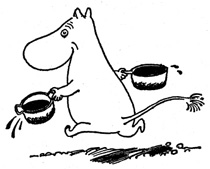
\includegraphics[width=209pt,height=169pt]{f0045-01.jpg}
\caption{}
\label{f0045-01}
\end{figure}

Kiam Mumintrolo revenis li etendis la transformitan akvon al sia patro dirante: ``Gustumu!''

Muminpatro trinkis gluton kaj mienis kontente. ``Kie vi akiris ĉi tion, filo?'' li demandis.

``Sekretoj!'' diris Mumintrolo.

Do ili plenigis konfitaĵujon per transformita akvo kaj frakasis ĝin kontraŭ la pruo de la velboato dum Muminpatrino kun fiero deklamis: ``Por tempo kaj nuno (muminesprimo uzata je baptoj) mi baptas vin `\emph{Aventuro}'.''

Ĉiuj hurais, kaj poste oni enboatigis korbojn, plejdojn, ombrelojn, fiŝvergojn, kovrilojn, kaserolojn kaj banŝortojn, kaj la muminfamilio forvelis kun siaj amikoj sur la sovaĝan, verdan maron.
\sectionbreak
Estis bela tago. Eble ne tute klara, ĉar maldensa brumo kovris la sunon. \emph{Aventuro} streĉis sian blankan velon kaj sagis direkte al la horizonto. Ondoj batis kontraŭ la flankoj de la boato kaj la vento kantis kaj martroloj kaj marfraŭlinoj dancis ĉirkaŭ la pruo.

Snif ligis siajn ses boatetojn en vico unu post la alia, kaj nun la tuta floto velis en la postakvo. La patro de Mumintrolo stiris kaj Muminpatrino sidis dormetante. Tre malofte ŝi havis tian kvieton ĉirkaŭ si. Super ili rondiris grandaj blankaj birdoj.

``Kien ni iru?'' demandis la snorko.

``Ni iru al insulo!'' petis Snorkfraŭlino. ``Mi neniam antaŭe estis sur insuleto!''

``Do ĉi-foje vi faros tion,'' diris la patro. ``Sur la unua vidata insulo ni albordiĝos.''

Mumintrolo sidis plej antaŭe ĉe la pruo gvatante al malprofundaĵoj. Li ravite gapis suben en la verdan profundon kie la pruo de \emph{Aventuro} tranĉis antaŭen kun blankaj lipharoj.

``Hej ho!'' vokis Mumintrolo ravite. ``Ni vojaĝos al insulo!''

Fore en la maro situis la soleca insulo de hatifnatoj, ĉirkaŭita de rifoj kaj surfoj. Unufoje jare la hatifnatoj kolektiĝis tie antaŭ ol denove ekiri en sia senfina vagado ĉirkaŭ la mondo. Ili alvenis el ĉiuj mondflankoj, silente kaj serioze, kun siaj etaj blankaj, malplenaj vizaĝoj. Kial ili jare kunvenas estas malfacile diri, ĉar ili povas nek aŭdi nek paroli kaj neniam okulfiksas ion ajn krom la forajn celojn al kiuj ili vojaĝas. Eble ili tamen ŝatas havi lokon kie ili hejmas kaj povas iom ripozi kaj renkonti konatojn. La jarkunveno ĉiam estas en junio, kaj do okazis tiel ke la muminfamilio kaj la hatifnatoj alvenis proksimume samtempe al la soleca insulo. Sovaĝa kaj alloga ĝi altiĝis el la maro, ornamita kaj kronita kvazaŭ por festo per blankaj surfoj kaj verdaj arboj.

``Tero antaŭe!'' kriis Mumintrolo. Ĉiuj klinis sin trans la boatrandon por rigardi.

``Troviĝas sablostrando!'' vokis Snorkfraŭlino.

``Kaj bona haveno!'' diris Muminpatro kaj elegante boardis inter rifoj ĝis la tero. \emph{Aventuro} mole ŝoviĝis en la sablon kaj Mumintrolo saltis surteren kun la ligŝnuro.

Baldaŭ la strando plenis de fervoro kaj agado. Muminpatrino kuntrenis ŝtonojn en fajrejon por varmigi la patkukon, ŝi kolektis brullignon kaj sternis la tablotukon sur la sablo kun eta ŝtono en ĉiu angulo por ke ĝi ne forbloviĝu. Ŝi vicigis ĉiujn tasojn kaj enfosis la buterujon en malsekan sablon en ombro de ŝtono kaj fine ŝi metis bukedon da strandlilioj meze de la tablo.

``Ĉu ni povas helpi vin pri io?'' demandis Mumintrolo kiam ĉio estis preta.

``Vi esploru la insulon,'' respondis la patrino (kiu sciis, ke tion ili sopiris). ``Estas grave scii kien oni trafis. Ĉi tie ja povas ekzisti danĝero.''

``Ĝuste,'' diris Mumintrolo. Kaj li ekiris kun la snorkaj gefratoj kaj Snif laŭ la suda bordo, dum Snufmumriko, kiu amis trovi aferojn sola, vagis laŭ la norda. La hemulo kunportis sian botanikan fosilon, sian verdan plantportujon kaj la grandigan lenson kaj vagis rekte en la arbaron. Li suspektis ke tie povas troviĝi strangaj plantoj kiun neniu ankoraŭ trovis.

Sed la patro de Mumintrolo sidiĝis sur ŝtonon por fiŝhoki. Kaj la suno malrapide rampis al posttagmezo dum fora nubaro densiĝis super la maro.

Meze de la insulo troviĝis verda maldensejo kun ebena tero ĉirkaŭata de florantaj veproj. Jen la hatifnatoj havis sian sekretan kunvenejon kie ili kolektiĝis unufoje jare je somermeza tempo. Proksimume tricent el ili jam alvenis kaj oni atendis ankoraŭ proksimume kvarcent kvindek. Ili silente rondiris sur la herbejo solene kapklinante unu al la alia. Meze de la maldensejo ili starigis altan foston, kaj sur tiu pendis granda barometro. Ĉiufoje preterpasante la barometron ili profunde kapklinis antaŭ ĝi (kio aspektis sufiĉe amuze).

Dume la hemulo vagadis en la arbaro, ravita pro la maloftaj floroj kiuj ĉie brilis. Ili ne similis la florojn de Muminvalo, ili havis pli intensajn kaj pli malhelajn kolorojn kaj strangan formon.

Sed la hemulo ne vidis ke ili estas belaj, li kalkulis stamenojn kaj foliojn kaj murmuris al si: ``Jen la ducentdeknaŭa numero en mia kolekto!''

\begin{figure}[htbp]
\centering
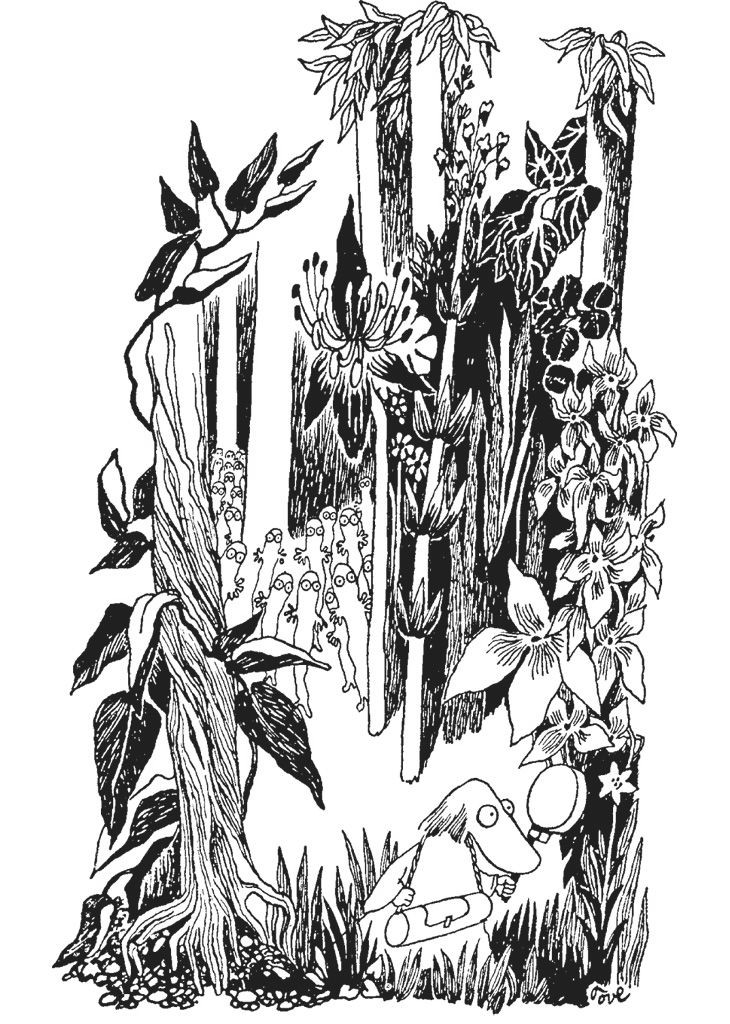
\includegraphics[width=450pt,height=631pt]{_14.jpg}
\caption{}
\label{_14}
\end{figure}

Fine li atingis la hatifnatan maldensejon kaj vagis en ĝin, fervore serĉante inter la herboj. La hemulo levis la rigardon nur kiam li frapis la kapon al la fosto de la hatifnatoj. Tiam li konsternite rigardis ĉirkaŭ si. Neniam en sia vivo li vidis tiom da hatifnatoj en unu loko. Ili svarmis ĉie, kaj ĉiuj gapis al li per siaj etaj palaj okuloj. `Mi demandas min ĉu ili estas koleremaj,' pensis la hemulo maltrankvile. `Ili ja estas etaj, sed ĝene multaj!'

Li rigardis la grandan brilan barometron el mahagono. Ĝi montris ``pluvon kaj venton.'' ``Mirige,'' diris la hemulo palpebrumante en la sunbrilo. Kaj li frapetis al la barometro kiu falis sufiĉe multe. Tiam la hatifnatoj minace susuris kaj faris paŝon kontraŭ la hemulo.

``Pro ĉio,'' diris la hemulo terurite. ``Mi certe ne prenos vian barometron!''

Sed la hatifnatoj ne aŭdis lin. Ili alproksimiĝis en vico post vico, susurante kaj flirtante per la manoj. La hemulo misglutis la koron kaj rigardis ĉirkaŭ si serĉante eblon savi sin. La malamikoj staris kvazaŭ muro ĉirkaŭ li kaj nur alproksimiĝis. Kaj inter la arbotrunkoj pluaj hatifnatoj alsvarmis, silentaj kaj kun senmovaj vizaĝoj. ``Foriru!'' kriis la hemulo. ``For! For!''

Sed la hatifnatoj silente alproksimiĝis. Tiam la hemulo kolektis siajn jupojn kaj ekgrimpis sur la foston. Ĝi estis glita kaj malagrabla, sed la teruriĝo donis al li malhemajn fortojn kaj fine li sidis tremante sur la pinto tenante la barometron.

La hatifnatoj atingis la piedon de la fosto. Tie ili atendis. La tuta maldensejo estis kovrita de ili kvazaŭ de blanka tapiŝo, kaj la hemulo malbonfartis pensante pri tio kio okazos al li se li falos suben.

``Helpu!'' li kriis per malforta voĉo. ``Helpu! Helpu!'' Sed la arbaro restis silenta.

Tiam li enigis du fingrojn enbuŝen kaj fajfis: tri mallongajn signalojn, tri longajn, tri mallongajn. Tri mallongajn, tri longajn, tri mallongajn. S.O.S.
\sectionbreak
Snufmumriko kiu vagis laŭ la norda bordo aŭdis la alarmsignalon de la hemulo. Kiam li distingis la direkton li tuj pafiĝis por helpi. La malproksima fajfo plilaŭtiĝis. `Nun estas tre proksime,' pensis Snufmumriko kaj singarde kaŝiris antaŭen. Heliĝis inter la arboj. Li vidis la maldensejon, la hatifnatojn kaj la hemulon kiu alkroĉis sin al la fosto. ``Ĉi tio estas pli aĉa afero,'' murmuris Snufmumriko. Poste li vokis: ``Saluton! Mi alvenis! Kiel vi tiel kolerigis la afablajn hatifnatojn?''

``Mi nur frapetis al ilia barometro,'' ĝemis la hemulo. ``Ĝi malaltiĝis, cetere. Klopodu forigi la abomenajn bestetojn, kara mumriko!''

``Mi devas pensi iom,'' diris Snufmumriko.

(De ĉi tiu interparolo la hatifnatoj aŭdis nenion, ĉar ili ja ne havas orelojn.)

Post iom vokis la hemulo: ``Pensu rapide, mumriko, ĉar mi baldaŭ glitos suben!''

``Aŭskultu!'' diris Snufmumriko. ``Ĉu vi memoras tiufoje kiam venis arvikoloj en la ĝardenbedon? Muminpatro enfosis amason da fostoj en la teron kaj surmetis ventohelicojn sur ilin. Kaj kiam la helicoj rondiris estiĝis vibrado en la tero tiel ke la arvikoloj nervoziĝis kaj foriris!''

``Viaj historioj ĉiam estas tre interesaj,'' diris la hemulo amare. ``Sed mi ne povas kompreni kiel ili rilatas al mia malĝojiga situo!''

``Sufiĉe multe,'' diris Snufmumriko. ``Ĉu vi ne komprenas? Hatifnatoj nek parolas nek aŭdas kaj vidas tre malbone. Sed ilia palpsento estas delikata! Provu balanci la foston tien-reen per etaj skuoj! La hatifnatoj certe sentos tion en la tero kaj ektimos. Tio iros rekte en ilian stomakon, komprenu!''

La hemulo klopodis balanci la foston tien-reen.

``Mi falos suben!'' li time ekkriis.

``Pli rapide, pli rapide!'' vokis Snufmumriko. ``Etaj, etaj skuoj!''

La hemulo balanciĝis tien-reen, kaj post iom la hatifnatoj ekhavis malagrablan senton en la plandoj. Ili susuris pli forte kaj malkviete moviĝis. Kaj subite ili fuĝis panike, precize kiel faris la arvikoloj.

En unu momento la maldensejo malpleniĝis. Snufmumriko sentis la hatifnatojn froti liajn krurojn irante en la arbaron, kaj ili bruligis precize kiel urtikoj.

La hemulo perdis la prenon pro pura trankviliĝo kaj falis suben sur la herbejon.

``Ho, mia kor'!'' li ĝemis. ``Nun denove ĝi saltis for en la gorĝon. Neniam estas io ajn krom bruo kaj danĝero de kiam mi venis en la muminfamilion!''

``Nun trankviliĝu,'' diris Snufmumriko. ``Vi ja bone saviĝis!''

``Abomenaj bestetoj!'' kverelis la hemulo. ``Ĉiuokaze mi kunportos ilian barometron por puni ilin!''

``Prefere lasu ĝin,'' avertis Snufmumriko.

Sed la hemulo dehokis la grandan brilan barometron kaj triumfe ŝovis ĝin sub la brakon.

``Nun ni reiru,'' li diris. ``Mi estas tute terure malsata.''

Kiam Snufmumriko kaj la hemulo revenis, ĉiuj aliaj manĝis ezokon kiun Muminpatro eligis el la maro.

``Saluton!'' vokis Mumintrolo. ``Ni rondiris la tutan insulon! Kaj ĉe la ekstera flanko troviĝas teruraj sovaĝaj rokoj kiuj subiras rekte en la maron.''

``Kaj ni vidis amason da hatifnatoj,'' rakontis Snif. ``Almenaŭ cent!''

``Ne parolu pri ili,'' diris la hemulo kun emfazo. ``Ĝuste nun mi ne eltenas tion. Sed jen vi vidos mian militan trofeon!'' Kaj la hemulo fiere lokis sian barometron meze de la manĝotablo.

``Ho,'' kiel brila kaj bela! ekkriis Snorkfraŭlino. ``Ĉu ĝi estas horloĝo?''

``Ne, ĝi estas barometro,'' diris Muminpatro. ``Per ĝi oni vidas ĉu estos bela vetero aŭ ŝtormo. Kelkfoje ĝi montras tute ĝuste!'' Li frapetis al la barometro kaj serioze sulkis la vizaĝon.

``\emph{Estos} ŝtormo!'' li diris.

``Ĉu granda ŝtormo?'' demandis Snif time.

``Rigardu mem,'' diris Muminpatro. ``La barometro indikas ``00'', kaj tio estas la plej malalta kiun barometro povas indiki. Se ĝi ne ŝercas al ni.''

Sed efektive ŝajnis kvazaŭ ĝi ne ŝercus. La brumo densiĝis en flavgriza nebulo, kaj fore ĉe la horizonto la maro estis strange nigra.

``Ni devas hejmeniri,'' diris la snorko.

``Ankoraŭ ne!'' petis Snorkfraŭlino. ``Ni ne havis tempon zorge esplori la rokojn de la ekstera flanko! Ni eĉ ne banis nin!''

``Ni ja povas atendi iomete por vidi kiel estos,'' diris Mumintrolo. ``Estus tia elreviĝo reiri hejmen kiam ni ĵus trovis ĉi tiun insulon!''

``Sed se estos ŝtormo ni tute ne povos iri,'' diris la snorko prudente.

``Tio estus plej bona!'' ekkriis Snif. ``Ni restos ĉi tie por ĉiam!''

``Silentu, idoj, mi devas pensi,'' diris la patro de Mumintrolo. Li iris ĝis la strando kaj flaris enaere, turnis la kapon ĉiudirekten kaj sulkis la frunton.

De fore aŭdiĝis tondrado.

``Fulmotondro!'' diris Snif. ``Hu, kiel terure!''

Super la horizonto altiĝis minaca nuba muro. Ĝi estis malhelblua kaj puŝis antaŭ si etajn helajn nubetojn. Jen kaj jen ekflamis pala lumo super la maro.

``Ni restos!'' decidis la patro.

``La tutan nokton!'' kriis Snif.

``Mi pensas ke jes,'' diris Muminpatro. ``Nun rapidu konstrui domon, ĉar la pluvo baldaŭ alvenos ĉi tien!''

Oni trenis \emph{Aventuron} alten sur la sablon, kaj ĉe la arbara rando oni rapidege faris domon el la velo kaj la plejdoj. Muminpatrino ŝtopis la flankojn per musko kaj la snorko fosis ĉirkaŭan fosaĵon por ke la pluvakvo havu ion en kion flui. Ĉiuj kuris tien-reen kaj savis siajn aĵojn sub la tegmenton. Nun venteto trairis la arbojn kiuj time susuris. La tondro aŭdiĝis pli proksime.

``Mi iros rigardi la veteron de sur la kabo,'' diris Snufmumriko. Li tiris la ĉapelon firme suben sur la orelojn kaj ekiris. Sola kaj feliĉa Snufmumriko plandis ĝis la plej ekstera kabo kaj ekstaris kun la dorso al granda ŝtono.

La maro ŝanĝis sian mienon. Nun ĝi estis nigre verda kaj portis ŝaŭmon sur la pintoj, kaj la rifoj lumis flave kiel fosforo. Solene muĝante la fulmotondro almarŝis de sude. Ĝi streĉis siajn nigrajn velojn super la maro, ĝi kreskis sur duonon de la ĉielo kaj la fulmoj malbonaŭgure flagris.

`Ĝi venos rekte super la insulon,' pensis Snufmumriko kun tremo de plezuro kaj ekscito. Li rigardis rekte en la fulmotondron kiu vagis antaŭen super la maro. Kaj subite Snufmumriko vidis etan nigran rajdanton sur nigra ĉevalo. Ili vidiĝis nur dum momento kontraŭ la krete blanka kresto de la nuba muro, la mantelo de la rajdanto disflugis kvazaŭ flugilo, ili plialtiĝis{\ldots} Poste ili malaperis en blindiga svarmo da fulmoj, la suno estis for kaj la pluvo alvenis kvazaŭ griza kurteno super la maro. `Mi vidis la sorĉiston!' pensis Snufmumriko. `Tio devis esti la sorĉisto kaj lia nigra pantero! Ili efektive ekzistas, ili ne estas nur malnova fabelo{\ldots}'

Snufmumriko turnis sin kaj saltis reen trans la strandon. Apenaŭ li atingis en la tendon. Pezaj gutoj jam batis la velan tolon kiu batis en la ŝtormo. Kvankam restis pluraj horoj ĝis la vespero, la tuta mondo vualiĝis en mallumon. Snif envolvis sin tuta en plejdon ĉar li timis la fulmotondron. La aliaj kaŭris unu apud la alia. La tendo odoris intense je la floroj de la hemulo.

Nun la tondro krakegis tute proksime. Fojon post fojo ilia kaŝejo pleniĝis de la blanka lumo de fulmoj. Muĝante la fulmotondro trenis siajn ferajn ĉarojn ĉirkaŭ la ĉielo, kaj la maro en furiozo ĵetis siajn plej grandajn ondojn kontraŭ la soleca insulo.

\begin{figure}[htbp]
\centering
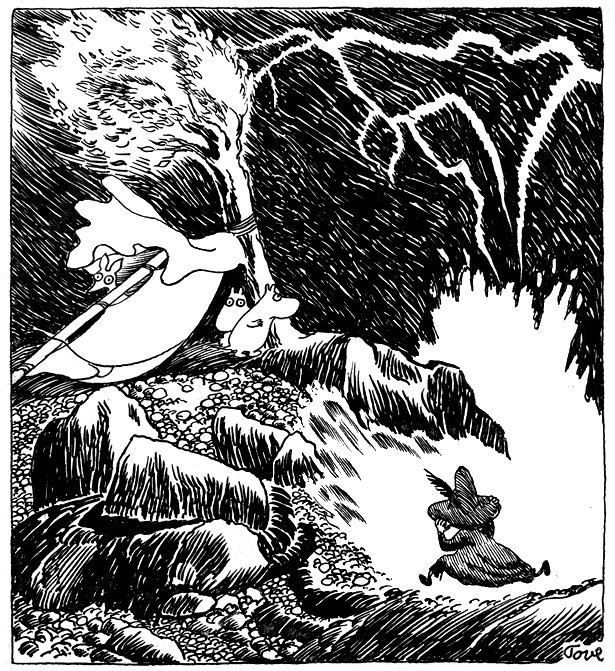
\includegraphics[width=450pt,height=492pt]{_15.jpg}
\caption{}
\label{_15}
\end{figure}

``Dank' al Dio ke ni ne estas surmare,'' diris Muminpatrino. ``Oj, oj, kia vetero.''

Snorkfraŭlino tremante ŝovis sian manon en tiun de Mumintrolo, kaj li sentis sin tre protektanta kaj vira.

Snif kuŝis kriante sub la plejdo.

``Nun ĝi estas rekte super ni!'' diris Muminpatro. Tiumomente siblanta fulmego fluis suben al la insulo, sekvate de klakanta tondro.

``Tiu trafis ion!'' diris la snorko.

Efektive \emph{estis} iom tro terure. La hemulo sidis tenante sian kapon. --

``Bruo! Ĉiama bruo!'' li murmuris.

Nun la fulmotondro iris suden. Pli kaj pli fore aŭdiĝis la tondrado, la fulmoj iĝis malpli intensaj. Fine nur pluvo susuris ĉirkaŭ ili kaj la maro muĝis ĉirkaŭ la bordoj.

`Mi ankoraŭ ne rakontos pri la sorĉisto,' pensis Snufmumriko. `Ili jam sen tio sufiĉe timas.'

``Elvenu, Snif,'' li diris. ``Ĉio pasis.''

Snif palpebrumante malimplikis sin el la plejdoj. Li estis iom embarasita ke li tiel terure kriis, kaj li oscedis kaj gratis sin malantaŭ la orelo. ``Kioma horo estas?'' li demandis.

``Baldaŭ la oka,'' diris la snorko.

``Do mi pensas ke ni enlitiĝu,'' diris la patrino de Mumintrolo. ``Ĉi tio estis sufiĉe emocia.''

``Sed ĉu ne estus ekscite esplori kien la fulmo trafis?'' diris Mumintrolo.

``Morgaŭ!'' diris lia patrino. ``Morgaŭ ni esploros ĉion kaj naĝos en la maro. Nun la insulo nur estas malseka kaj griza kaj malagrabla.'' Kaj ŝi alĝustigis la plejdojn ĉirkaŭ ili kaj endormiĝis kun sia mansako sub la kuseno.

Ekstere la ŝtormo kreskis. Strangaj sonoj eniĝis en la muĝadon de ondoj. Voĉoj kaj kurantaj piedoj, rido kaj sonorado de grandaj sonoriloj surmare. Snufmumriko kuŝis senmova aŭskultante kaj sonĝante kaj memoris siajn vojaĝojn ĉirkaŭ la mondo. Baldaŭ mi devos ekiri refoje,' li pensis. `Sed ankoraŭ ne.'

\chapter[Kvara Ĉapitro]{}


\begin{figure}[htbp]
\centering
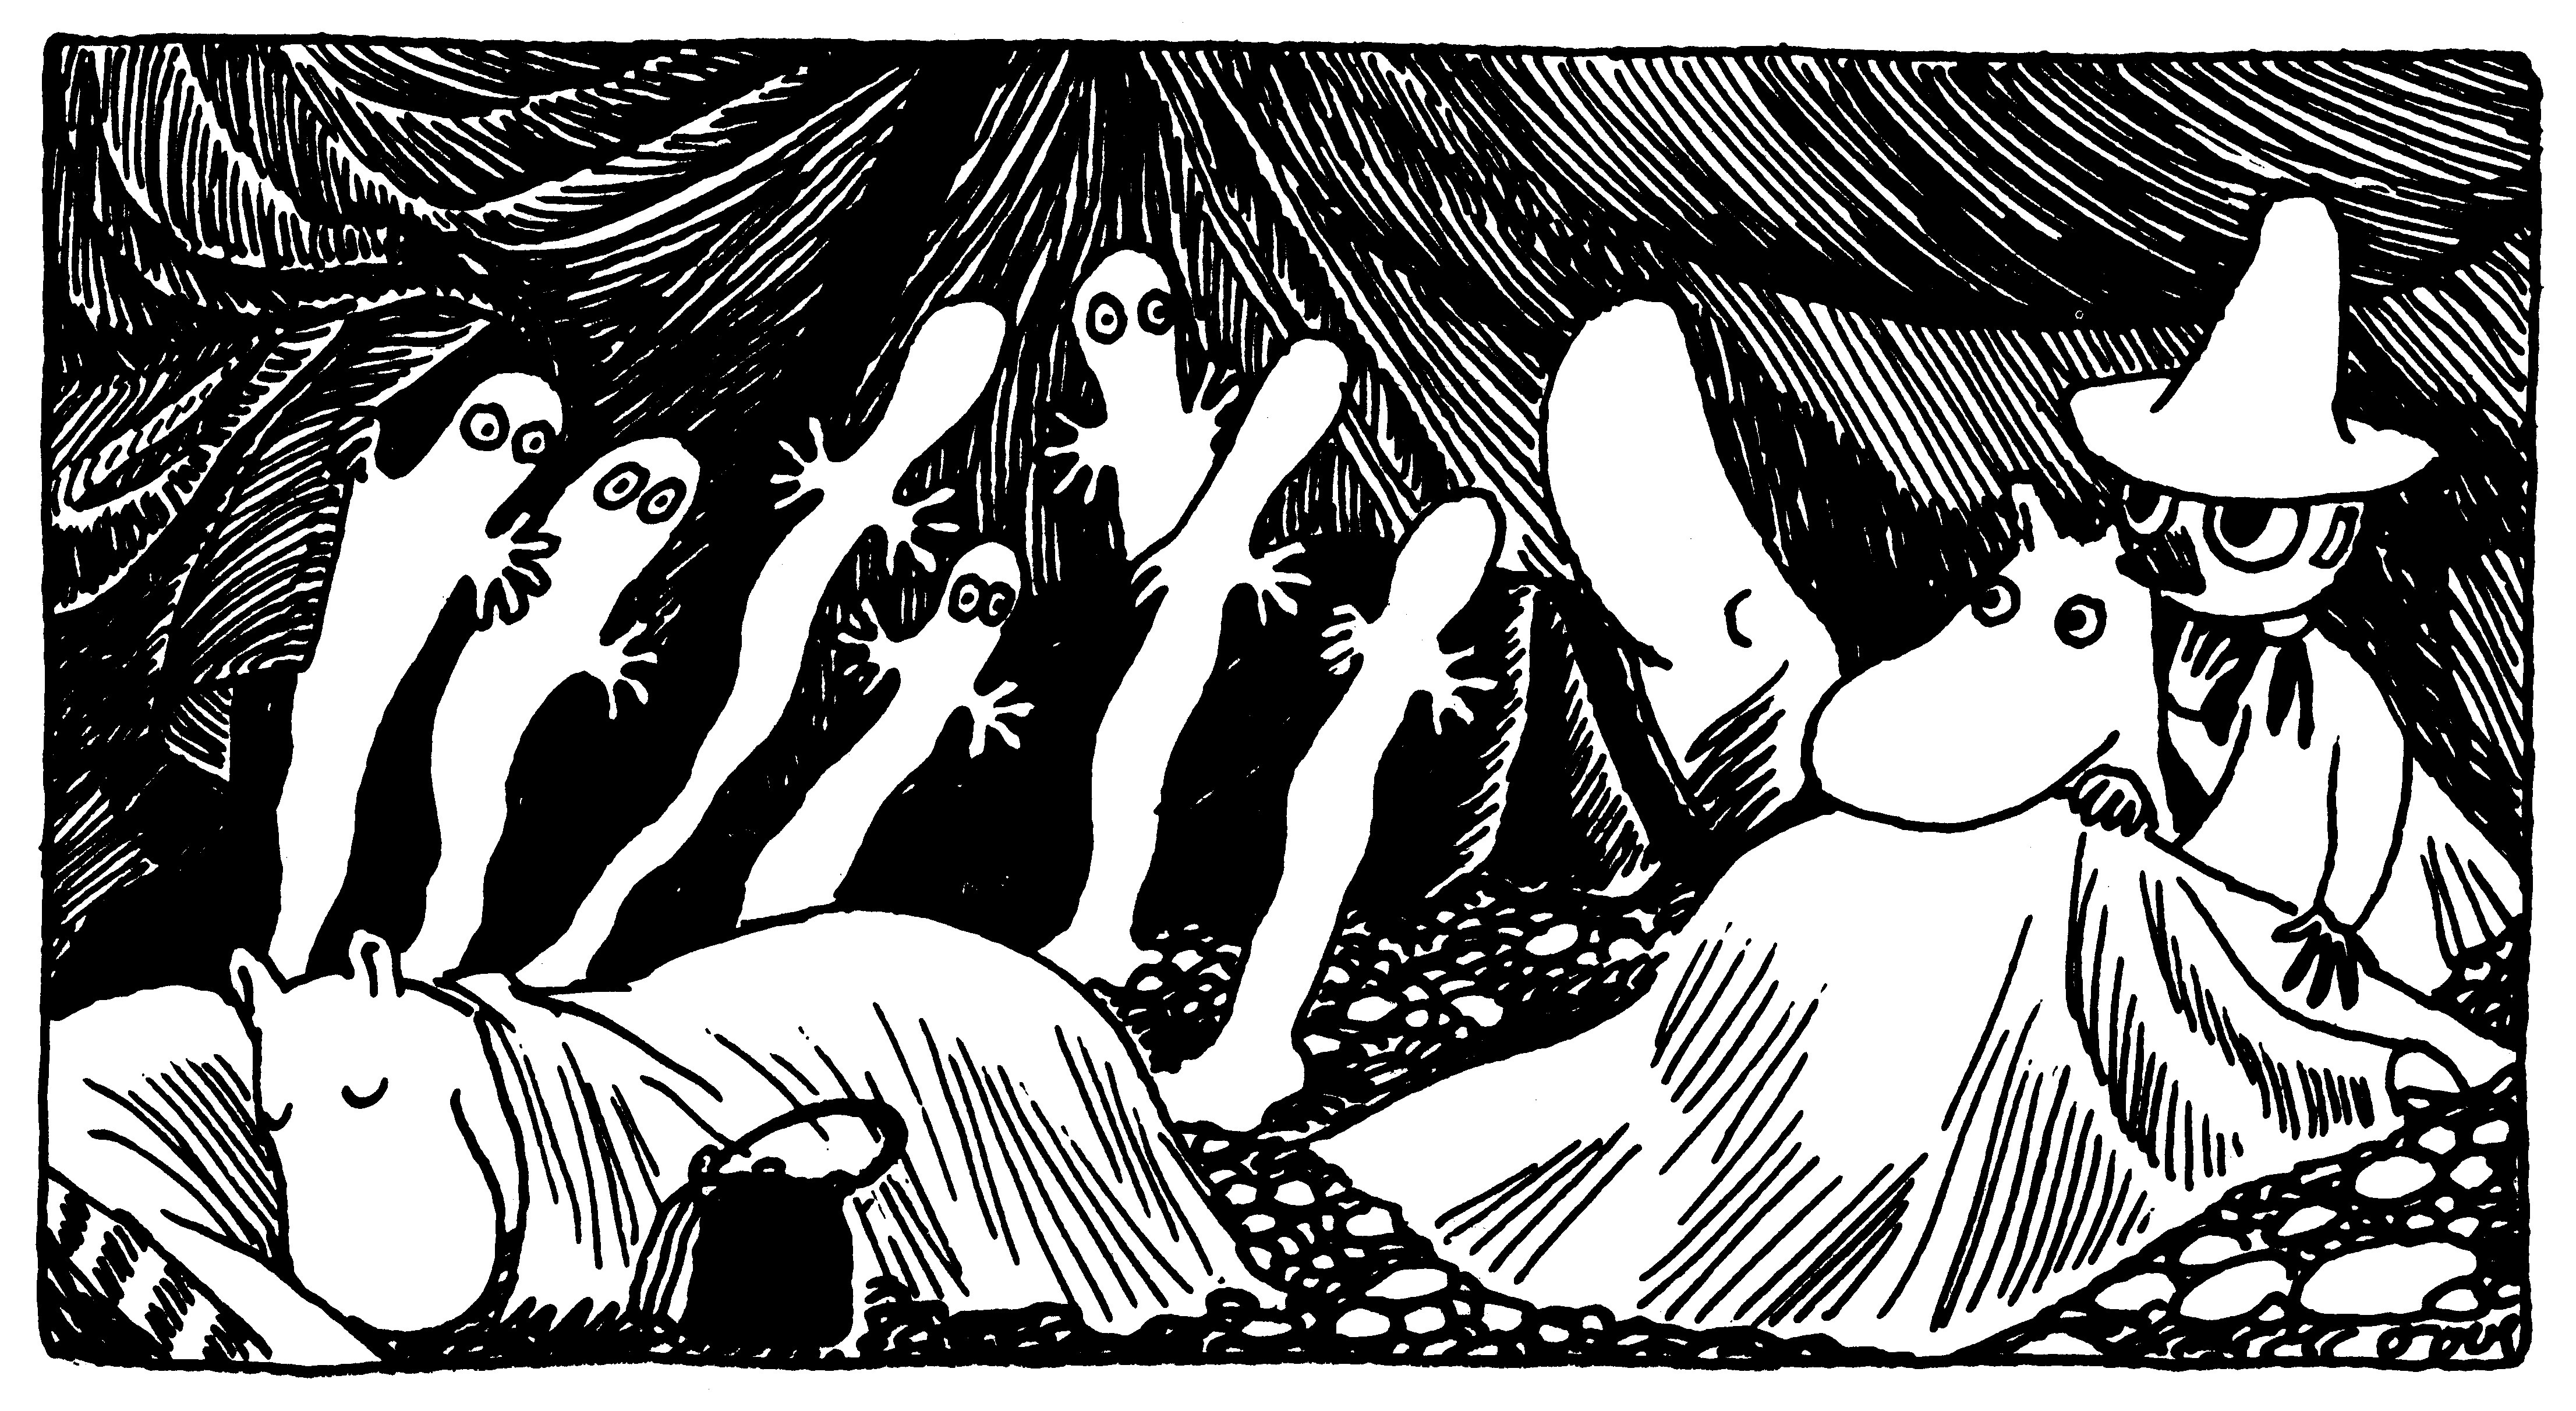
\includegraphics[width=450pt,height=246pt]{_16.jpg}
\caption{}
\label{_16}
\end{figure}

\begin{center}\textbf{\Large\color{ForestGreen}\textsc{Kvara Ĉapitro}}\end{center}

\noindent\textit{en kiu Snorkfraŭlino kalviĝas dum la nokta atako de hatifnatoj, kaj en kiu oni rakontas pri la ege mirigaj surstrandaj trovoj faritaj sur la soleca insulo.}
\hfill \break
\hypertarget{Kvara Ĉapitro}{}
\label{Kvara Ĉapitro}


\noindent Meze de la nokto Snorkfraŭlino vekiĝis kun terura sento. Io tuŝis ŝian vizaĝon. Ŝi ne kuraĝis rigardi sed maltrankvile flaris ĉirkaŭ si. Odoris je brulo! Snorkfraŭlino tiris la kovrilon super la kapon kaj vokis duonvoĉe: ``Mumintrolo, Mumintrolo!''

Mumintrolo tuj vekiĝis. Kio estas? li demandis.

``Io danĝera envenis!'' diris Snorkfraŭlino sub la kovrilo. ``Mi \emph{sentas} ke troviĝas io danĝera ĉi tie!''

Mumintrolo gapis en la mallumon. Jen estis io! Etaj lumoj{\ldots} Pale lumaj estaĵoj kiuj plandis tien-reen inter la dormantoj. Mumintrolo skue vekis Snufmumrikon.

``Rigardu!'' li terurite flustris. ``Fantomoj!''

``Ne,'' diris Snufmumriko. ``Tio estas la hatifnatoj. La fulmotondro igis ilin elektraj --- tial ili lumas. Restu tute senmova, alie vi povos sperti elektran frapon!''

La hatifnatoj ŝajne serĉis ion. Ili esploris ĉie en la korboj kaj la brulodoro plifortiĝis. Subite ili ĉiuj kolektiĝis en la angulo kie la hemulo dormis.

``Ĉu vi pensas ke ili volas ataki lin?'' demandis Mumintrolo ekscitite.

``Kredeble ili nur serĉas la barometron,'' diris Snufmumriko. ``Mi avertis lin kunporti ĝin. Nun ili trovis ĝin!''

Kun komuna penado la hatifnatoj eligis la barometron. Ili surtretis la hemulon por pli bone kapti ĝin, kaj nun la brula haladzo atingis foren.

Snif vekiĝis kaj komencis ĝemi. Subite la tendo pleniĝis de kriego. Iu hatifnato hazarde tretis sur la nazon de la hemulo.

En momento ĉiuj vekiĝis kaj stariĝis. Estiĝis nepriskribebla malordo. Timaj demandoj miksiĝis kun plendaj hurloj kiam iu tretis sur hatifnatoj kaj brulvundiĝis aŭ spertis elektran frapon. La hemulo kuradis en rondo kriante pro teruriĝo, kaj subite li implikiĝis en la velon kaj la tendo renversiĝis sur ilin. Estis vere terure.

Snif poste asertis ke daŭris almenaŭ horon ĝis ili trovis la vojon eksteren el la velo (eventuale li iomete troigis).

Sed kiam ili finfine liberigis sin de ĝi, la hatifnatoj jam malaperis en la arbaron kun la barometro. Kaj neniu emis persekuti ilin.

La hemulo dum laŭta ĝemado ŝovis sian nazon en la malsekan sablon. ``Tio transiras la limon!'' li diris. ``Kial iu kompatinda senkulpa botanikisto ne povas vivi sian vivon en paco kaj kvieto?''

``La vivo ne estas paca,'' diris Snufmumriko gaje.

``Ĉesis pluvi,'' diris Muminpatro. ``Rigardu, idoj, la ĉielo estas klara! Baldaŭ tagiĝos.''

La patrino de Mumintrolo frostetis firme tenante sian mansakon. Ŝi rigardis al la ŝtorma, nokta maro. ``Ĉu ni faru novan domon kaj provu reendormiĝi?'' ŝi demandis.

``Ne indas,'' diris Mumintrolo. ``Ni volvu nin en la plejdojn kaj atendu ĝis la suno leviĝos.''

Do ili sidiĝis en vico surstrande, proksime unu apud la alia. Snif volis sidi en la mezo, ĉar li trovis tion plej sekura.

``Vi ne povas imagi kiel timige estis kiam io tuŝis mian vizaĝon en la mallumo,'' diris Snorkfraŭlino. ``Tio estis pli terura ol la fulmotondro!''

\begin{figure}[htbp]
\centering
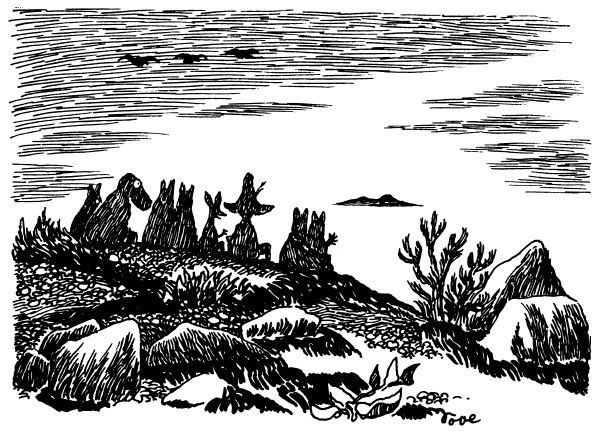
\includegraphics[width=449pt,height=325pt]{_17.jpg}
\caption{}
\label{_17}
\end{figure}

Ili sidis rigardante al la maro en la heliĝanta nokto. La ŝtormo iom kvietiĝis, sed ankoraŭ surfoj muĝante ruliĝis al la sablo. La ĉielo komencis paliĝi en oriento kaj estis tre malvarme. Kaj tiam, en la unua tagiĝo, ili vidis la hatifnatojn ekiri de la insulo. Boato post boato ekglitis kvazaŭ ombroj de trans la kabo kaj direktiĝis foren sur la maro.

``Bone!'' diris la hemulo. ``Espereble mi neniam plu devos vidi hatifnaton.''

``Ili sendube elserĉos novan insulon,'' diris Snufmumriko. ``Sekretan insulon kiun neniu iam ajn trovos!'' Kaj per rigardoj de sopiro li okulsekvis la malpezajn boatojn de la etaj mondvagantoj.

Snorkfraŭlino dormis kun la kapo sur la genuoj de Mumintrolo. Nun la unua lumstrio vidiĝis ĉe la orienta horizonto. Kelkaj nubetoj kiujn la ŝtormo postlasis iĝis helruĝaj kiel rozoj, kaj jen la suno levis sian brilan kapon el la maro.

Mumintrolo klinis sin por veki Snorkfraŭlinon kaj tiam li malkovris ion teruran. Ŝiaj belaj fruntharoj estis forbruligitaj! Tio sendube okazis kiam la hatifnato tuŝis ŝin. Kion ŝi diros, kiel li povos trankviligi kaj konsoli ŝin? Tio estis katastrofo!

Snorkfraŭlino malfermis la okulojn ridetante.

``Sciu,'' diris Mumintrolo rapide. ``Estas sufiĉe strange pri mi. Kun la paso de tempo mi komencis pli ŝati fraŭlinojn sen haroj ol tiujn kun haroj!''

``Ĉu?'' diris Snorkfraŭlino surprizite. ``Kial?''

``Aspektas tiel senzorge kun haroj!'' diris Mumintrolo.

Snorkfraŭlino tuj levis la manojn por kombi sin -- sed ve! la sola afero kiun ŝi trovis estis eta bruligita tufo. Ŝi gapis al ĝi kun profunda teruro.

``Vi kalviĝis,'' diris Snif.

``Tio vere konvenas al vi,'' konsolis Mumintrolo. ``Ho ne, ne ploru!''

Sed Snorkfraŭlino ĵetis sin sur la sablon kaj ploris torentojn da larmoj pro la perdo de sia ĉefa ĉarmaĵo.

Ĉiuj kolektiĝis ĉirkaŭ ŝi por provi reĝojigi ŝin. Vane!

``Vidu, mi naskiĝis kalva,'' diris la hemulo. ``Kaj mi efektive tre ŝatas tion!''

``Ni ŝmiros oleon sur vin kaj ĝi certe ree elkreskos,'' diris la patro de Mumintrolo.

``Kaj tiam ĝi estos bukla!'' diris Muminpatrino.

``Ĉu tio estas vera?'' singultis Snorkfraŭlino.

``\emph{Certe} tio estas vera!'' promesis la patrino. ''Nur imagu kiel bela vi estos kun buklaj haroj!

Snorkfraŭlino ĉesis plori kaj eksidis.''

``Rigardu la sunon,'' diris Snufmumriko. Ĵusbanita kaj bela ĝi leviĝis el la maro. La tuta insulo glimis kaj brilis post la pluvo. ``Nun mi ludos matenan kanton,'' diris Snufmumriko kaj elpoŝigis sian buŝharmonikon. Kaj oni kantis plenforte:

\begin{center}\itshape "Post blovata nokta hor',  
hatifnato iris for!  
Jen la fino de koŝmar':  
Snorkfraŭlino kun bukla har'!  
Hej ho! "\\\end{center}

``Ek al la ban'!'' vokis Mumintrolo. Kaj ĉiuj surmetis banŝortojn kaj kuris en la surfon (krom la hemulo kaj la gepatroj de Mumintrolo, kiuj trovis ĝin ankoraŭ tro malvarma).

Vitre verdaj kaj blankaj la ondoj ruliĝis sur la sablon. Ho, esti ĵusvekiĝinta mumintrolo kaj danci en vitre verdaj ondoj dum la suno leviĝas! La nokto estis forgesita kaj nova longa juna tago kuŝis antaŭ ili. Kiel marporkoj ili sagis rekte tra la ondoj kaj velis sur iliaj krestoj al la strando kie Snif ludis en la malprofunda akvo. Snufmumriko flosis surdorse pli foren kaj rigardis en la ĉielon kiu estis blua kaj travidebla.

\begin{figure}[htbp]
\centering
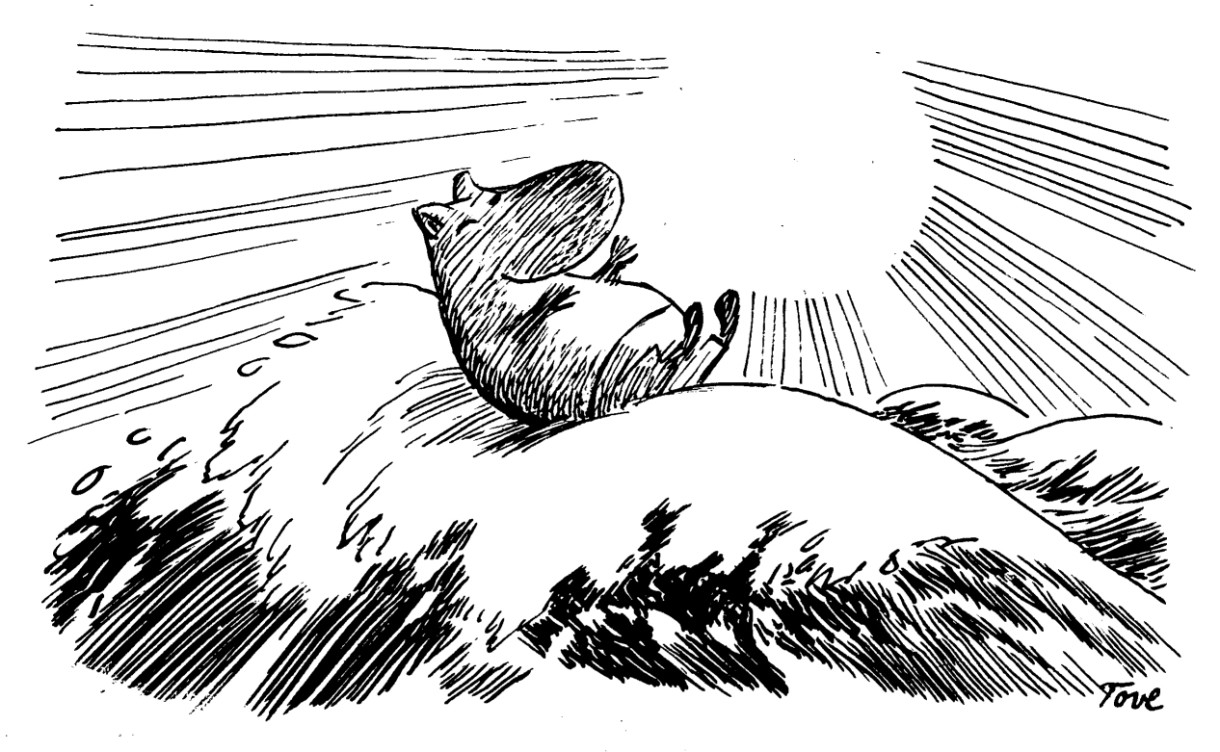
\includegraphics[width=447pt,height=276pt]{_18.jpg}
\caption{}
\label{_18}
\end{figure}

Dume la patrino de Mumintrolo kuiris kafon inter la ŝtonoj kaj serĉis la buterujon kiun ŝi kaŝis de la sunbrilo en la strandakvo. Sed ŝi serĉis vane, la ŝtormo forportis ĝin. ``Kion mi donu al ili sur la pano,'' plendis la patrino.

``Vi vidos ke la ŝtormo donos al ni ion alian rekompence,'' diris Muminpatro. ``Post la kafo ni faru esplorvagadon laŭ la bordoj por vidi kion la maro surterigis!'' Kaj tion ili faris.

Ĉe la ekstera flanko de la insulo la praroko levis siajn glate poluritajn dorsojn el la maro. Inter ili oni povis neatendite trovi pecetojn da sablo punktita de konkoj, la kaŝitan dancejon de la marfraŭlinoj, aŭ nigrajn misterajn fendegojn, kie la surfo muĝis kvazaŭ batoj al fera pordo. Jen malfermiĝis eta groto inter la rokoj, jen ili falis krute suben kontraŭ ronda lavpelvo el siblantaj akvokirloj.

\begin{figure}[htbp]
\centering
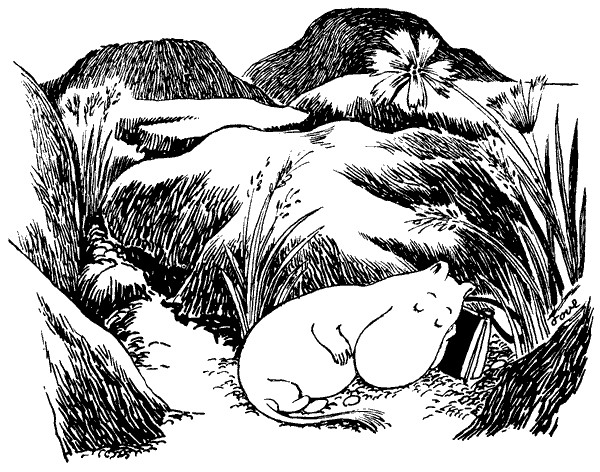
\includegraphics[width=449pt,height=355pt]{_19.jpg}
\caption{}
\label{_19}
\end{figure}

Ĉiu ekiris sola por serĉi strandajn trovaĵojn kaj vrakerojn. Estis pli ekscite ol io ajn alia, ĉar eblis trovi la plej strangajn aĵojn, kaj ofte estis sufiĉe malfacile kaj danĝere savi ilin el la maro.

La patrino de Mumintrolo grimpis suben al eta sablejo kiu situis ŝirmita de grandegaj ŝtonblokoj. Sur la sablo kreskis aroj da bluaj sablaj diantoj kaj mara aveno kiu raslis kaj siblis kiam la vento penetris en la mallarĝajn kanojn. Muminpatrino kuŝiĝis ŝirmite de la ŝtormo. Ĉi-sube ŝi vidis nur la bluan ĉielon kaj la sablajn diantojn kiuj balanciĝis super ŝia kapo. `Mi ripozos nur dum kelka tempo,' ŝi pensis. Sed baldaŭ la patrino dormis profunde sur la varma sablo.

Sed la snorko kuris supren sur la plej altan monton kaj rigardis ĉirkaŭ si. Li povis vidi de bordo al bordo, kaj la insulo ŝajnis al li flosi kiel bukedo sur la malkvieta maro. Jen vidiĝis Snif kiel punkteto serĉadi vrakerojn, jen li videtis la verdan ĉapelon de Snufmumriko -- jen la hemulo elfosis maloftan orkidon{\ldots} Kaj jen! Jen absolute kie la fulmo trafis! Grandega ŝtonbloko, pli granda ol dek mumindomoj, estis fendita kvazaŭ pomo de la fulmo kaj ambaŭ duonoj falis flanken kaj malfermis vertikalan fendegon inter si. Tremante la snorko enpaŝis en la fendegon kaj rigardis supren al la malhelaj rokaj flankoj. Jen la fulmo trairis! Nigra kiel karbo ĝia vojo desegniĝis en la nudigitan internon de la ŝtono. Sed apud ĝi iris alia strio kiu estis hela kaj brila! Ĝi estis oro, ĝi povis esti nenio alia ol oro!

La snorko pikis en la strion per sia tranĉilo. Eta orgrajno malfiksiĝis kaj falis en lian manon. Li forigis pecon post peco. Li varmegiĝis pro fervoro kaj forhakis pli kaj pli grandajn pecojn. Kaj post iom la snorko jam forgesis ĉion alian krom la radiantaj orvejnoj kiujn la fulmo nudigis. Li ne plu estis marborda rabisto, li estis orfosisto!

Dume Snif faris tre simplan trovon, sed ĝi almenaŭ same ĝojigis lin. Li trovis kork-zonon. Ĝi estis iom borita de la marakvo sed precize konvenis al li. `Nun mi povos ekiri en profundan akvon!' pensis Snif. Nun mi certe lernos naĝi same bone kiel la aliaj. Kiel Mumintrolo surpriziĝos! Iom pli fore, inter betulŝelo, fiŝoretaj flosiloj kaj fukoj li trovis bastmaton kaj preskaŭ sendifektan ĉerpilon kaj malnovan boton sen kalkanumo. Mirindaj trezoroj se oni rabis ilin de la maro! De malproksime Snif ekvidis Mumintrolon kiu staris enakve tirante kaj trenante ion. Ion grandan!

`Mizere ke mi ne ekvidis ĝin unua!' pensis Snif. `Kio ajn ĝi povas esti!'

Nun Mumintrolo savis sian marbordan trovaĵon kaj rulis ĝin antaŭ si sur la sablo. Snif streĉis, streĉadis la kolon -- kaj nun li vidis kio ĝi estas. Buo! Granda bela buo!

``Hej ho!'' vokis Mumintrolo. ``Kion vi nun diras?''

``Ĝi estas sufiĉe bona,'' diris Snif kritike kun la kapo oblikve. ``Sed kion vi pensas pri ĉi tiuj?''

Kaj li vicigis \emph{siajn} trovaĵojn sursable.

``La korko-zono estas bona,'' diris Mumintrolo. ``Sed kion fari per duona ĉerpilo?''

``Tio certe funkcias se oni ĉerpas rapide,'' diris Snif. ``Aŭskultu! Kion vi dirus pri interŝanĝo? La bastmato, ĉerpilo kaj boto kontraŭ tiu malnova buo?''

``Neniam,'' diris Mumintrolo. ``Sed eble la kork-flosilo kontraŭ ĉi tiu mistera talismano kiu alflosis de fora lando.'' Kaj li altiris strangan objekton el kava vitro kaj skuis ĝin. Tiam amaso da neĝflokoj ekflirtis ene de la vitrobulo kaj denove kuŝiĝis en paco sur etan domon kun fenestroj el arĝenta papero.

``Ho,'' diris Snif. Kaj furioza batalo okazis en lia koro kiu ege tro multe amis posedaĵojn.

``Rigardu!'' diris Mumintrolo kaj refoje skuis la neĝon.

``Mi ne scias,'' ekkriis Snif senespere, ``mi vere ne scias kio plej plaĉas al mi, la savzono aŭ la vintra talismano! Mia koro krevas!''

``Ĝi sendube estas la sola neĝa talismano kiu troviĝas surtere ĝuste nun,'' diris Mumintrolo.

``Sed mi ne \emph{povas} rezigni la naĝzonon!'' ĝemis Snif. ``Kara Mumintrolo, ĉu ni ne povas dividi la etan neĝfalon!''

``Hm,'' diris Mumintrolo.

``Ĉu mi ne povus almenaŭ teni ĝin kelkfoje,'' petis Snif. ``En la dimanĉoj?''

Mumintrolo iom cerbumis. Poste li diris: ``Jes. Vi povas havi ĝin dimanĉe kaj merkrede.''
\sectionbreak
Fore de tie vagis Snufmumriko. Li paŝis kiel eble plej proksime al la siblantaj ondoj, kaj kiam ili mordetis al liaj ŝuoj li forsaltis ridante. Tio estis sufiĉe moka al ili!

Iom for de la kabo Snufmumriko renkontis la patron de Mumintrolo kiu okupiĝis savi trunkstumpojn kaj tabulojn.

``Bone, ĉu ne?'' spiregis Muminpatro. El ĉi tio mi konstruos varfon por \emph{Aventuro}!

``Ĉu mi helpu vin surterigi ilin?'' demandis Snufmumriko.

``Ne, ne!'' diris Muminpatro timigite. ``Tion mi mem kapablas. Provu trovi ion propran por surterigi!''

Ĉi tie troviĝis multo por savi el la maro sed nenio pri kio Snufmumriko zorgis. Bareletoj, duona seĝo, senfunda korbo kaj gladostablo. Pezaj, ĝenaj aĵoj. Snufmumriko enpoŝigis la manojn kaj fajfis. Li forsaltis de la ondoj kaj postkuris ilin mokante. Kaj kiam ili volis kapti lin, li denove forsaltis. Laŭ la tuta longa, soleca sablostrando.

Sed fore sur la kabo Snorkfraŭlino grimpadis inter la rokoj. Ŝi kaŝis siajn bruligitan fruntajn lanugojn sub krono el marlilioj kaj serĉis bordan trovaĵon kiu surprizos la aliajn kaj igos ilin enviaj. Kaj post kiam ili admiros ĝin ŝi donacos ĝin al Mumintrolo (se ĝi ne iel rilatas al juveloj, kompreneble). Estis malfacile grimpi inter la ŝtonoj, kaj la krono senĉese volis forbloviĝi de ŝi. Ĉiuokaze nun ŝtormis malpli. La maro ŝanĝis siajn kolerajn verde siblajn kolorojn al kviete bluaj, kaj la ondoj portis siajn ŝaŭmkrestojn pli multe kiel ornamon ol kiel minacon. Snorkfraŭlino krablis suben sur mallarĝa gruzbenko kiu borderis la akvorandon. Sed tie troviĝis nenio krom iom da fukoj kaj kanoj kaj kelkaj tabulstumpoj. Mishumore ŝi vagis plu direkte al la kabo.

``Estas malĝojige ke la aliaj efektivigas tiel multe sed mi ne,'' diris Snorkfraŭlino al si enpense. ``Ili saltas sur glacipecoj kaj digas riveretojn kaj kaptas formik-leonojn. Mi ŝatus fari ion mirigan, tute sola kun mi mem kaj imponi al Mumintrolo.''

Suspirante ŝi rigardis al la dezerta strando. Kaj tiam ŝi subite haltis kaj ŝia koro ekbatis. Plej fore sur la kabo{\ldots} Ho, ne, tio estas tro terura! Iu kuŝis plaŭdante kontraŭ la strandaj ŝtonoj kun la kapo subakve! Kaj iu estis ege granda, dekoble tiel granda kiel la eta Snorkfraŭlino!

`Mi tuj kuros venigi la aliajn,' ŝi pensis. Sed ŝi ne kuris.

``Nun vi ne denove estu malkuraĝa!'' diris Snorkfraŭlino al si. ``Vi devas rigardi kiu estas tiu! Kaj tremante ŝi alproksimiĝis al la teruraĵo.''

Estis granda sinjorino{\ldots} Granda sinjorino sen kruroj{\ldots} kiel terure! Snorkfraŭlino faris kelkajn tremantajn paŝojn kaj haltis en plej granda surpriziĝo. La granda sinjorino estis farita el ligno! Kaj ŝi estis mirinde bela. Tra la klara akvo lumis ŝia trankvila, ridetanta vizaĝo kun ruĝaj vangoj kaj lipoj, kaj la rondaj bluaj okuloj estis vaste malfermitaj. Ankaŭ la haroj estis bluaj, ili serpentis en longaj pentritaj bukloj sur la ŝultroj. ``Ŝi estas reĝino,'' diris Snorkfraŭlino ravite. La manoj de la bela sinjorino kuŝis kruce sur la brusto kiu brilis de oraj floroj kaj ĉenoj, kaj de la maldika talio la robo fluis en molaj, ruĝaj faldoj. Kaj ĉio estis el pentrita ligno. La sola strangaĵo estis ke ŝi ne havis dorson.

\begin{figure}[htbp]
\centering
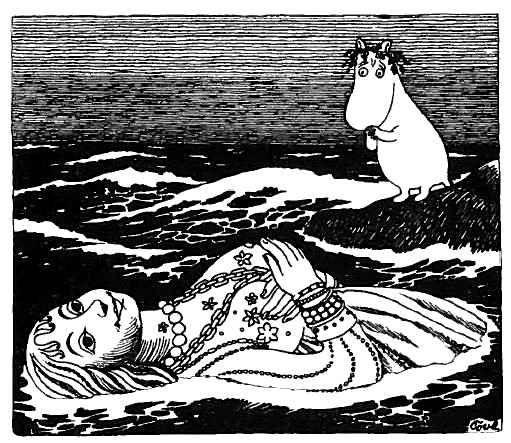
\includegraphics[width=448pt,height=390pt]{_20.jpg}
\caption{}
\label{_20}
\end{figure}

``Ŝi preskaŭ estas tro bela donaco por Mumintrolo,'' cerbumis Snorkfraŭlino. ``Sed li tamen ricevos ŝin!'' Estis fiera Snorkfraŭlino kiu je la vesperiĝo pagajis en la boatgolfon, sidante sur la ventro de la ligna reĝino.

``Ĉu \emph{vi} trovis boaton?'' demandis la snorko.

``Imagu ke vi povis venigi ĝin ĉi tien tute sola,'' admiris Mumintrolo.

``Ĝi estas ŝipobeka figuro!'' diris Muminpatro kiu estis surmare en sia junaĝo. ``La maristoj kutimas ornami la pruon de la ŝipo per bela reĝino el ligno.''

``Kial?'' demandis Snif.

``Por esti tre belaj,'' diris la patro.

``Sed kial ŝi ne havas dorson?'' scivolis la hemulo.

``Jen kie ŝi estas fiksita al la pruo, kompreneble,'' diris la snorko. ``Tion ja ĵusnaskita musido povas kompreni!''

``Ŝi estas ege tro granda por esti najlita al \emph{Aventuro},'' diris Snufmumriko.

``Ege domaĝe!''

``Ho, la bela sinjorino!'' suspiris la patrino de Mumintrolo. ``Imagu, esti tiel bela kaj ne havi ian plezuron el tio!''

``Kion vi faros pri ĝi?'' demandis Snif.

Snorkfraŭlino mallevis la rigardon kaj ridetis. Poste ŝi diris: ``Mi donacos ĝin al Mumintrolo.''

Mumintrolo povis eldiri eĉ ne unu vorton. Tute ruĝvizaĝa li antaŭeniris kaj kapklinis. Snorkfraŭlino konfuzite riverencis kaj la tuta afero aspektis kvazaŭ ili estus en festeno.

``Fratino,'' diris la snorko. ``Vi ne vidis kion \emph{mi} trovis!''

Kaj li fiere montris al granda brilanta amaso da oro kuŝanta sursable.

La okuloj de Snorkfraŭlino elstaris. ``Vera oro!'' ŝi spiris.

``Troviĝas multe, multe pli!'' fanfaronis la snorko. ``Monto el oro!''

``Kaj \emph{mi} rajtas kolekti ĉion kio defalas per si mem kaj havi ĝin kiel mian propran,'' diris Snif.

Ho, kiom oni admiris la trovaĵojn unu de la aliaj surstrande! Subite la muminfamilio riĉiĝis. Sed la plej valora tamen estis la ŝipobeka figuro kaj la eta neĝado en la vitra globo.

\begin{figure}[htbp]
\centering
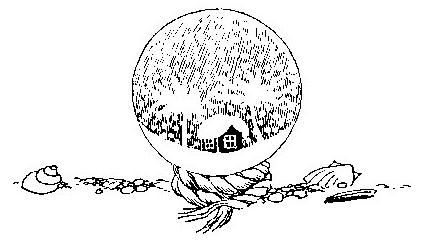
\includegraphics[width=200pt,height=112pt]{_21.jpg}
\caption{}
\label{_21}
\end{figure}

Estis peze ŝarĝita velboato kiu fine ekiris for de la soleca insulo tra la postŝtorma hulado. Malantaŭ ĝi treniĝis granda floso el trunkoj kaj tabuloj, kaj la ŝarĝo konsistis el oro kaj vintra talismano, granda bela buo, boto, duona ĉerpilo, savzono kaj bastmato, kaj ĉe la pruo kuŝis la ŝipobeka figuro rigardante foren al la maro. Apud ŝi sidis Mumintrolo tenante manon sur ŝia bela blua hararo. Li estis tiel feliĉa!

Snorkfraŭlino de temp' al tempo rigardis ilin.

`Ho, se mi estus same bela kiel la ligna reĝino,' ŝi pensis. `Nun mi eĉ ne plu havas mian fruntan lanugon{\ldots}' Ŝi ne sentis sin same ĝoja kiel ĵus.

Ne, ŝi estis preskaŭ malĝoja.

``Ĉu vi ŝatas la lignan reĝinon?'' ŝi demandis.

``Tre!'' respondis Mumintrolo ne levante la rigardon.

``Sed vi ja diris ke vi ne ŝatas fraŭlinojn kun haroj,'' diris Snorkfraŭlino. ``Cetere ŝi estas nur pentrita!''

``Sed tiel bele pentrita!'' diris Mumintrolo.

Snorkfraŭlino malĝojis. Ŝi rigardis suben en la maron dum ploro ŝtopis ŝian gorĝon kaj ŝi malrapide griziĝis. ``La ligna reĝino aspektas stulte!'' ŝi diris kolere.

Tiam Mumintrolo levis la rigardon.

``Kial vi estas griza?'' li demandis surprizite.

``Pro nenio!'' diris Snorkfraŭlino.

Tiam Mumintrolo foriris el la pruo kaj sidiĝis apud ŝin.

``Sciu,'' li diris post iom. ``La ligna reĝino efektive aspektas ege stulte!''

``Jes, ĉu ne?'' diris Snorkfraŭlino kaj refariĝis rozkolora.

La suno malrapide malaltiĝis en vesperon kaj la longaj brilaj huloj estis kolorigataj flave kaj ore. Ĉio iĝis flava kaj ora, la velo, la boato, kaj tiuj kiuj sidis en ĝi.

``Ĉu vi memoras la oran papilion kiun ni vidis?'' demandis Mumintrolo.

Snorkfraŭlino kapjesis, laca kaj feliĉa.

Malproksime la soleca insulo flamis en la sunsubiro.

``Mi scivolas kion vi faros el la oro de la snorko?'' diris Snufmumriko.

``Ni metos ĝin kiel ornamon ĉirkaŭ la florbedoj,'' diris la patrino de Mumintrolo. ``La pli grandajn pecojn, kompreneble, ĉar la etaj aspektas kiel rubaĵo.''

Poste ĉiuj silentis kaj rigardis al la suno kiu subiris en la maron dum la koloroj paliĝis en bluon kaj violkoloron kaj \emph{Aventuro} malrapide balanciĝis hejmen.

\begin{figure}[htbp]
\centering
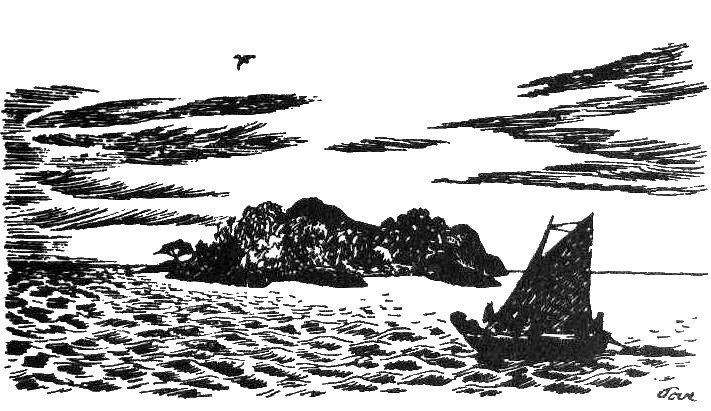
\includegraphics[width=450pt,height=259pt]{_22.jpg}
\caption{}
\label{_22}
\end{figure}

\chapter[Kvina Ĉapitro]{}


\begin{figure}[htbp]
\centering
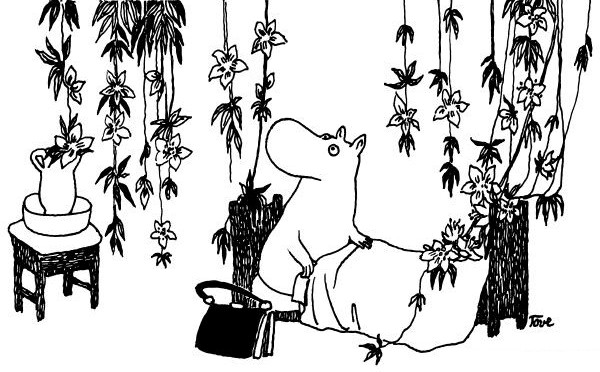
\includegraphics[width=450pt,height=278pt]{_26.jpg}
\caption{}
\label{_26}
\end{figure}

\begin{center}\textbf{\Large\color{ForestGreen}\textsc{Kvina Ĉapitro}}\end{center}

\noindent\textit{en kiu oni parolas pri la Reĝa Rubeno, pri la fiŝado per longa hokarfadeno de la snorko kaj la morto de la mamluko, kaj pri kiel la mumindomo transformiĝis en ĝangalon.}
\hfill \break
\hypertarget{Kvina Ĉapitro}{}
\label{Kvina Ĉapitro}


\noindent Estis iam en la fino de julio, kaj en Muminvalo estis tre varmege. Eĉ ne la muŝoj havis forton zumi. La arboj ŝajnis lacaj kaj polvaj, la rivero sekiĝis kaj fluis mallarĝa kaj bruna tra velkantaj herbejoj. La akvo ne plu taŭgis por fari sukon en la ĉapelo de sorĉisto (kiu denove estis akceptita kaj staris sur la komodo sub la spegulo).

Tagon post tago la suno brilis rekte suben al la valo kiu kuŝis kaŝita inter montetoj. Ĉiuj bestetoj krablis en siajn malvarmajn tunelojn, kaj la birdoj silentis. Sed la amikoj de Mumintrolo nervoziĝis pro la varmo kaj rondiris kverelante unu kun la alia.

``Panjo,'' diris Mumintrolo, ``elpensu al ni ion por fari! Ni nur kverelas kaj estas tiel varme!''

``Jes, kara infano,'' diris Muminpatrino. ``Mi rimarkis tion. Mi eble ŝatus dum kelka tempo esti sen vi. Ĉu vi ne povus transloĝiĝi en la groton dum kelkaj tagoj? Tie estas malpli varme kaj vi povus kuŝi enmare por trankviliĝi dum la tuta tago se vi volus.''

``Ĉu ni rajtas ankaŭ \emph{dormi} en la groto?'' demandis Mumintrolo ĝoje.

``Jes ja!'' diris la patrino. ``Kaj ne revenu hejmen antaŭ ol vi estos gajaj.''

Estis tre ekscite serioze \emph{ekloĝi} en la groto. Meze sur la sablogrundo ili metis la petrollampon. Ĉiu fosis kavon kiu konvenis al lia aparta formo kaj dorma pozo kaj tie sternis kuŝejon. La manĝoprovizoj estis dividitaj en ses egalajn amasojn. Troviĝis sekvinbera pudingo kaj kukurba kaĉo, bananoj, striaj mentbombonoj kaj maizo kaj krome patkuko por la morgaŭa matenmanĝo.

Vespere venteto ekblovis kaj solece flugis super la mara strando. La suno subiris ruĝe kaj plenigis la groton per sia varma lumo. Snufmumriko ludis krepuskajn kantojn kaj Snorkfraŭlino kuŝis kun sia bukla kapo sur la genuoj de Mumintrolo. Ĉiu sentis sin bonvola post la sekvinbera pudingo, kaj estis tute konvene timige vidi la krepuskon ŝteliri de trans la maro.

``Mi estas tiu kiu iam trovis la groton,'' diris Snif.

Kaj neniu zorgis diri ke tion ili jam centfoje aŭdis.

``Ĉu vi kuraĝas aŭdi ion teruran?'' demandis Snufmumriko kaj eklumigis la lampon.

``Kiom teruran?'' scivolis la hemulo.

``Proksimume kiel de ĉi tie ĝis la pordo aŭ iom pli foren,'' diris Snufmumriko. ``Se tio ion signifas al vi.''

``Ne, male,'' diris la hemulo. ``Nur rakontu, kaj mi avertos kiam mi ektimos.''

``Bone,'' diris Snufmumriko. ``(Nun vi aŭdos historion kiun iu gafsino rakontis al mi kiam mi estis infano.) Ĉe la fino de l' mondo situas kapturne alta monto. Ĝi estas fulge nigra kaj silke glata. Ĝi deklivas krute suben kie troviĝas neniu fundo kaj la nuboj glisas ĉirkaŭ ĝi. Sed plej alte surpinte situas la domo de l' sorĉisto, kaj ĝi aspektas ĉi tiel.'' Kaj Snufmumriko desegnis la domon en la sablo.

``Ĉu ĝi ne havas fenestrojn?'' demandis Snif.

``Ne,'' diris Snufmumriko. ``Nek pordon, ĉar la sorĉisto ĉiam revenas hejmen rajdante sur nigra pantero. Li ĉiam rajdadas nokte kolektante rubenojn en sia mantelo.''

\begin{figure}[htbp]
\centering
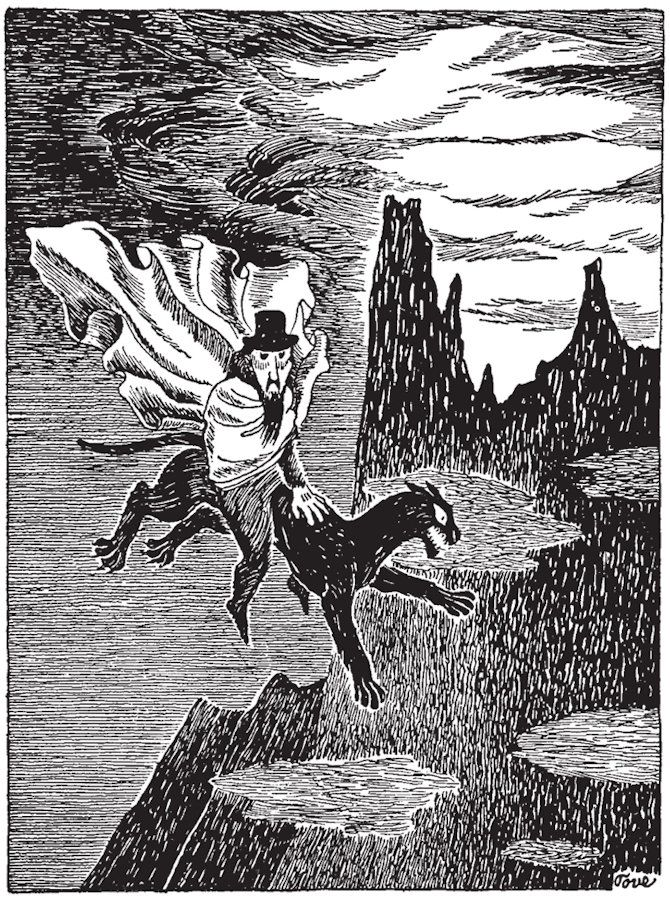
\includegraphics[width=450pt,height=604pt]{_23.jpg}
\caption{}
\label{_23}
\end{figure}

``Kion vi diras?'' vokis Snif kun elstaraj oreloj. ``Rubenojn? Kiel li trovas ilin?''

``La sorĉisto povas transformiĝi en ion ajn,'' diris Snufmumriko. ``Kaj li povas eniĝi en la teron kaj ĝis la marfundo kie troviĝas la kaŝitaj trezoroj.''

``Kion li faras per tiom da gemoj?'' demandis Snif envie.

``Nenion. Li nur kolektas ilin,'' diris Snufmumriko. ``Proksimume kiel la hemulo kolektas plantojn.''

``Ĉu vi diris ion?'' ekkriis la hemulo kaj vekiĝis en sia sablokavo.

``Mi rakontis ke la sorĉisto havas domon plenan de rubenoj,'' diris Snufmumriko. ``Ili kuŝas en grandegaj amasoj kontraŭ la muroj kaj estas enkrustitaj en la muroj kvazaŭ okuloj de sovaĝbestoj. La domo de la sorĉisto ne havas tegmenton kaj la nuboj kiuj flugas super ĝi estas ruĝaj kiel sango pro rebrilo de la rubenoj. Ankaŭ liaj propraj okuloj estas ruĝaj kaj brilas en mallumo.''

``Nun mi baldaŭ ektimos,'' diris la hemulo. ``Rakontu singarde, mi petas!''

``Kiel feliĉa li devas esti, tiu sorĉisto,'' suspiris Snif.

``Tute ne,'' diris Snufmumriko. ``Ne ĝis li trovos la Reĝan Rubenon. Ĝi estas preskaŭ same granda kiel la kapo de la nigra pantero, kaj rigardi en ĝin estas kiel vidi likvan fajron. La sorĉisto serĉis la Reĝan Rubenon sur ĉiuj planedoj, eĉ sur Neptuno -- sed li ne trovis ĝin. Li ekiris al la luno por serĉi en la krateroj, sed li ne havas grandan esperon sukcesi. Ĉar plej interne la sorĉisto kredas ke la Reĝa Rubeno troviĝas sur la suno. Kaj tien li ne povas veni. Li provis plurfoje, sed estas tro varmege. Kaj tio estas kion la gafsino rakontis al mi.''

``Tio estas bona rakonto,'' diris la snorko. ``Donu al mi plian mentbombonon.''

Snufmumriko dum kelka tempo silentis. Poste li diris: ``Ne estas rakonto. Ĉio estas vera.''

``Mi ĉiam kredis ke ĝi estas vera,'' ekkriis Snif. ``Tio pri la gemoj sonas tiel reala!''

``Kaj kiel eblas scii ke la sorĉisto ekzistas?'' demandis la snorko malkredeme.

``Mi vidis lin,'' diris Snufmumriko kaj ekbruligis sian pipon. ``Mi vidis la sorĉiston kaj lian panteron sur la insulo de hatifnatoj. Ili rajdis tra la aero meze de la fulmotondro.''

``Sed vi nenion diris!'' ekkriis Mumintrolo.

Snufmumriko levis la ŝultrojn. ``Plaĉas al mi havi sekretojn,'' li diris. ``Cetere, la gafsino rakontis ke la sorĉisto estas vestita en nigra cilindra ĉapelo.''

``Ĉu vi certas?'' kriis Mumintrolo.

``Devas esti tiu!'' volis Snorkfraŭlino.

``Efektive,'' diris la snorko.

``Kio?'' scivolis la hemulo. ``Pri kio vi parolas?''

``Pri la ĉapelo, kompreneble,'' diris Snif. ``La nigra cilindra ĉapelo kiun mi trovis ĉi-printempe! La sorĉa ĉapelo! Ĝi sendube forbloviĝis de li kiam li flugis al la luno!''

Snufmumriko kapjesis.

``Sed imagu se la sorĉisto revenos por preni sian ĉapelon,'' diris Snorkfraŭlino ekscitite. ``Mi neniam kuraĝus rigardi liajn ruĝajn okulojn!''

``Li kredeble restas sur la luno,'' diris Mumintrolo. ``Ĉu estas longa vojo tien?''

``Sufiĉe,'' diris Snufmumriko. ``Cetere li supozeble bezonos longan tempon por traserĉi ĉiujn kraterojn.''

Estis kelktempa maltrankvila silento. Ĉiuj pensis pri la nigra ĉapelo kiu staris hejme sur la komodo sub la spegulo.

``Iomete altigu la lampon,'' diris Snif.

``Ĉu vi aŭdis ion?'' flustris Snorkfraŭlino. ``Ekstere{\ldots}''

Ili gapis al la nigra enirejo de la groto kaj aŭskultis. Etaj, etaj, malpezaj sonoj -- ĉu eble la plandaj paŝoj de pantero?

``Estas pluvo,'' diris Mumintrolo. ``La pluvo alvenis. Nun ni iom dormu''.

Kaj ili kuŝiĝis ĉiu en sian sablokavon volvante la kovrilojn ĉirkaŭ si.

Mumintrolo estingis la lampon, kaj je la malforta susuro de pluvo li englitis en dormon.
\sectionbreak
La hemulo vekiĝis pro tio ke lia dormkavo estis plena de akvo. La varma somera pluvo flustris ekster la groto, ĝi fluis riverete kaj akvofale laŭ la muroj, kaj ĉiu akvo kiu troviĝis ekstere kaj interne fluis ĝuste en lian dormkavon.

``Mizero, mizero,'' diris la hemulo al si. Poste li vringis la akvon el sia robo kaj iris eksteren por rigardi la veteron. Ĉie estis same, grize kaj malseke kaj mizere. La hemulo pripensis ĉu li emas bani sin, sed li ne emis.

`Neniam estas ordo en la mondo,' pensis la hemulo malgaje. `Hieraŭ estis tro varmege kaj nun estas tro malseke. Mi iru enen por rekuŝiĝi.'

La dormkavo de la snorko ŝajnis plej seka.

``Movu vin for,'' diris la hemulo. ``Pluvis en mian liton.''

``Plej malbone por vi mem,'' diris la snorko kaj turnis sin sur la alian flankon.

``Tial mi intencas dormi en via kavo,'' klarigis la hemulo. ``Bonvolu malsnorkiĝi!''

Sed la snorko nur iom grumblis kaj dormis plu. Tiam venĝemo plenigis la koron de la hemulo, kaj li fosis kanalon tra la sablo inter sia propra dormkavo kaj tiu de la snorko.

``Tio estis malhemaĵo,'' diris la snorko kaj sidiĝis sub sia malseka kovrilo. ``Sed mi neniam kredus ke vi povas elpensi ion tiel ruzan!''

``Tio okazis per si mem,'' diris la hemulo gaje. ``Kaj kion ni do faru hodiaŭ?''

La snorko eligis la nazon tra la grota enirejo por rigardi la ĉielon kaj la maron. Poste li diris kompetente: ``Fiŝado. Veku la domon kaj mi iros prepari la boaton!''

Kaj la snorko marŝis suben sur la malsekan sablon kaj sur la varfon kiun konstruis la patro de Mumintrolo. Li flaris kelkan tempon al la maro.

Estis tute kviete, la pluvo malintense falis kaj ĉiu guto faris delikatan ringon sur la brila akvo. La snorko kapjesis al si mem kaj elportis la plej grandan skatolon kun longa hokarfadeno el la boatejo.

Poste li eltiris la fiŝujon de sub la varfo kaj sidiĝis surmeti logaĵon sur la hokojn dum li fajfis la ĉasokanton de Snufmumriko.

\begin{figure}[htbp]
\centering
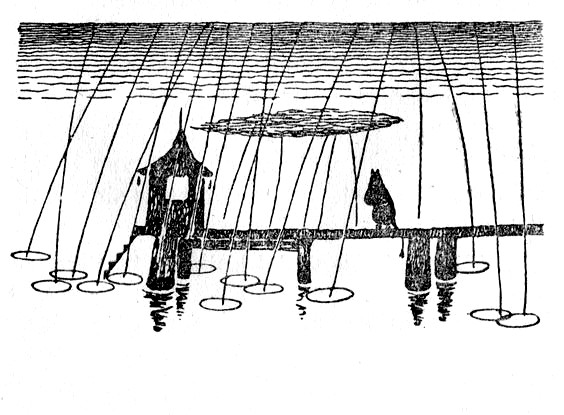
\includegraphics[width=448pt,height=330pt]{_24.jpg}
\caption{}
\label{_24}
\end{figure}

La tuta skatolo estis preta kiam la aliaj venis el la groto.

``Nu, jen vi finfine estas,'' diris la snorko. ``Hemulo, faligu la maston kaj enigu la remilingojn.''

``Ĉu ni \emph{devas} fiŝi?'' demandis lia fratino. ``Neniam io okazas kiam ni fiŝas, kaj mi tiel domaĝas la etajn ezokojn.''

``Bone, sed hodiaŭ \emph{io} okazos,'' diris la snorko. ``Sidiĝu ĉe la pruo kie vi malplej ĝenas.''

``Lasu min helpi,'' kriis Snif kaj kaptis la hokarfadenan skatolon. Li saltis suben sur la boatrandon, la boato ekbaskulis kaj jen la hokarfadena skatolo kuŝiĝis renversite sur la boatfundon kun duono de sia enhavo implikita al la remilingo kaj la ankro.

``Eminente,'' diris la snorko. ``Tute eminente. Sperta pri la maro, kvieta en boatoj kaj ĉio tia. Respekto al la laboro de aliaj, antaŭ ĉio. Ha.''

``Ĉu vi ne riproĉos lin?'' scivolis la hemulo surprizite.

``Riproĉos? Mi?'' diris la snorko kaj malgaje ridis. ``Ĉu ŝipestroj rajtas ion diri? Neniam. Vi bonvolu enakvigi la skatolon kia ĝi estas, sendube io alkroĉiĝos.'' Kaj la snorko enrampis sub la poban sidbenkon kaj tiris ŝirmotukon super la kapon.

``Kia aĉaĵo!'' diris Mumintrolo. ``Prenu la remilojn, mumriko, kaj ni malimplikos la mizeraĵon. Snif, vi estas azeno.''

``Jes ja,'' diris Snif dankeme. ``En kiu fino ni komencu?''

``Meze,'' diris Mumintrolo. ``Sed ne impliku ankaŭ la voston en la aferon.''

Kaj Snufmumriko malrapide remis \emph{Aventuron} eksteren sur la maron.
\sectionbreak
Dum ĉio ĉi okazis la patrino de Mumintrolo rondiris en sia domo kun ege kontenta sento. La pluvo milde susuris sur la ĝardeno. Paco, ordo kaj silento regis ĉie.

``Kiom ĉio kreskos!'' diris la patrino al si. Kaj ho, kiel agrable havi ilin en la groto! Ŝi ekhavis la ideon iomete ordigi kaj komencis kolekti ŝtrumpojn, oranĝoŝelojn, strangajn ŝtonojn, pecojn da arboŝelo kaj similajn aferojn. En la muzika skatolo ŝi trovis kelkajn kriptogamojn kiujn la hemulo forgesis meti en la plantopremilon. La patrino buligis ilin dum ŝi penseme aŭskultis la mallaŭtan susuradon de la pluvo. Kiom ĉio kreskos! ŝi ripetis kaj lasis la bulon fali elmane. Ĝi falis rekte suben en la ĉapelon de sorĉisto, sed tion Muminpatrino ne rimarkis. Ŝi retiriĝis en sian ĉambron por dormi, ĉar troviĝis nenio kion ŝi tiel amis kiel endormiĝi dum pluvo falas sur la tegmenton.

Sed en la profundo de la maro la longa hokarfadeno de la snorko embuskis. Ĝi jam kuŝis de kelkaj horoj kaj Snorkfraŭlino preskaŭ mortis pro enuo.

``Gravas la ekscito,'' klarigis Mumintrolo. ``\emph{Povas} esti io sur ĉiu hoko, komprenu.''

Snorkfraŭlino iom suspiris.'' Sed tamen,'' ŝi diris. ''Kiam oni enakvigas la hokon troviĝas duono de blankfiŝo sur ĝi kaj kiam oni elakvigas ĝin troviĝas tuta perko. Oni scias ke estos tuta perko. ''

``Aŭ nenio ajn!'' diris Snufmumriko.

``Aŭ lofio,'' diris la hemulo.

``Tion ne komprenas inoj,'' finis la snorko. ``Nun ni povas komenci elakvigi. Sed neniu rajtos krii. Malrapide! Malrapide!''

La unua hoko elakviĝis.

Ĝi estis malplena.

La dua hoko elakviĝis.

Ankaŭ ĝi estis malplena.

``Tio nur pruvas ke ili iras profunde,'' diris la snorko. ``Kaj estas grandegaj. Nun silentu, ĉiuj.''

Li ekigis ankoraŭ kvar malplenajn hokojn kaj diris: ``Ĝi estas ruzulo. Ĝi prenas niajn logaĵojn. Terure granda ĝi devas esti.''

Ĉiuj klinis sin trans la boatrando gapante en la nigran profundon kien la hokarfadeno kondukis.

``Kia fiŝo ĝi povas esti laŭ vi?'' demandis Snif.

``Mamluko, minimume,'' diris la snorko. ``Nun rigardu jene, ankoraŭ dek malplenaj hokoj!''

``Nu ja,'' diris Snorkfraŭlino.

``Nu ja al vi!'' diris ŝia frato kolere kaj haŭlis plu. ``Silentu ĉiuj, alie ni fortimigos ĝin!''

Hoko post hoko estis alkroĉata al la skatolo. Tufoj da marherbo kaj fuko. Neniu fiŝo. Absolute nenio ajn.

Subite kriis la snorko: ``Atentu! Io tiras! Mi estas absolute certa ke io tiras!''

``La mamluko!'' kriis Snif.

``Nun vi \emph{devas} regi vin,'' diris la snorko strebante resti trankvila. ``Tomba silento! Jen ĝi venos!''

La streĉita fadeno malstreĉiĝis, sed profunde en la malhelverdo io blanka glimis. Ĉu la pala fiŝventro de mamluko? Kvazaŭ montodorso el la sekreta pejzaĝo de la mara fundo io altiĝis kontraŭ la surfacon{\ldots} io grandega, minaca, senmova. Verda kaj muska kiel la trunko de arbego ĝi glitis supren sub la boato.

``La kaptsako!'' kriis la snorko. ``Kie la kaptsako?''

Kaj tiumomente la aero pleniĝis de muĝado kaj blanka ŝaŭmo. Enorma ŝvelondo levis \emph{Aventuron} sur sian kreston kaj renversis la hokarfadenan skatolon sur la boatfundon. Poste ĉio same subite rekvietiĝis.

Nur la ŝirita fadeno pendis melankolie sur la boatrando, kaj grandegaj akvokirloj markis la vojon de la monstro.

\begin{figure}[htbp]
\centering
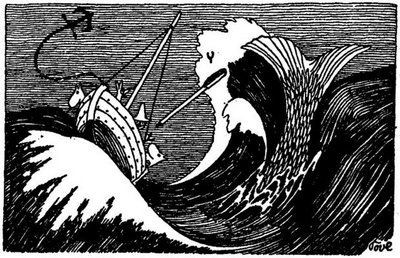
\includegraphics[width=449pt,height=291pt]{_25.jpg}
\caption{}
\label{_25}
\end{figure}

``Ĉu vi \emph{nun} pensas ke ĝi estas perko?'' la snorko demandis sian fratinon kun tre aparta tono. ``Tian fiŝon mi \emph{neniam} plu ricevos. Kaj vere ĝoja mi ankaŭ ne estos.''

``Jen kie ĝi ŝiriĝis,'' diris la hemulo kaj levis la fadenon. ``Io diras al mi ke la fadeno estis tro maldika.''

``Iru bani vin,'' diris la snorko kaŝante la okulojn en la mano.

La hemulo volis diri ion, sed Snufmumriko piedbatis lian kruron. Tute silentiĝis en la boato. Tiam Snorkfraŭlino delikate diris: ``Imagu se ni farus duan provon? La ligŝnuro certe eltenos?''

La snorko elsnufis. ``Post iom li murmuris: Kaj la hoko?''

``Via poŝtranĉilo,'' diris Snorkfraŭlino. ``Se vi disfaldas ambaŭ tranĉilojn, la korktirilon, la ŝraŭbilon kaj la alenon ĝi ja devos ie alkroĉiĝi?''

La snorko forprenis la manon de la okuloj kaj diris: ``Jes, sed la logaĵo?''

``La patkuko,'' diris lia fratino.

La snorko kelkan tempon konsideris la aferon dum ĉiuj retenis la spiron pro ekscitiĝo. Fine li diris: ``Bone, se la mamluko manĝas patkukojn,'' kaj tiam oni sciis ke la ĉaso daŭros.

Ili firme ligis la poŝtranĉilon al la ligŝnuro per peco da drato kiun la hemulo havis enpoŝe, fiksis la patkukon sur la tranĉilo kaj enigis ĉion en la maron. Ili atendis en silento.

Subite \emph{Aventuro} ekbaskulis.

``Ŝŝŝŝ!'' diris la snorko. ``Ĝi ekmordas!'' Ankoraŭ skuo. Pli bruska. Kaj poste sekvis fortega ektiro kiu ĵetis ilin ĉiujn boatfunden.

``Helpu!'' kriis Snif. ``Ĝi manĝos nin!''

\emph{Aventuro} trempis la nazon en la maron sed restariĝis kaj ekiris plenrapide foren sur la maron. La ligŝnuro etendiĝis streĉite kiel kordo antaŭen, kaj kie ĝi malaperis en la akvon leviĝis du blankaj lipharoj el ŝaŭmo.

Evidente la mamluko ŝatis patkukon.

``Trankvile!'' kriis la snorko. ``Kviete en boatoj! Ĉiu persono en sia posteno!''

``Espereble ĝi ne plonĝos!'' vokis Snufmumriko kiu rampis ĝis la pruo.

Sed la mamluko iris rekte antaŭen, pli kaj pli foren sur la maro. Baldaŭ la strando kuŝis kiel mallarĝa strio malantaŭ ili.

``Kiel longe vi pensas ke ĝi havos forton daŭrigi?'' demandis la hemulo.

``En plej aĉa okazo ni povos tranĉi la ŝnuron,'' diris Snif. ``Alie tio okazos je via risko!''

``Neniam!'' ekkriis Snorkfraŭlino skuante sian fruntan lanugon.

Nun la mamluko svingis sian enorman voston enaere, turniĝis kaj reiris kontraŭ la bordon.

``Nun tio iras iom malpli rapide,'' kriis Mumintrolo kiu genuis ĉe la pobo kontrolante la postakvon. ``Ĝi laciĝas!''

La mamluko estis laca, sed ĝi ankaŭ plikoleriĝis. Ĝi skuis la ŝnuron kaj turnis tien-reen tiel ke \emph{Aventuro} balanciĝis en la plej danĝerega maniero.

Jen ĝi estis tute senmova por trompi ilin, kaj jen ĝi ekiris per tia forto ke la ŝvelondoj superfluis la pruon. Tiam Snufmumriko elpoŝigis sian buŝharmonikon kaj ludis sian ĉasokanton dum la aliaj piedbatis la takton tiel ke la boatfundo tremis. Kaj vidu! En la sama momento la mamluko turnis sian grandegan ventron supren.

Pli granda neniam ekzistis. Ili rigardis ĝin dum silenta momento. Poste diris la snorko: ``Mi tamen kaptis ĝin!''

``Jes!'' diris lia fratino fiere.

Dum oni trenis la mamlukon al la tero la pluvo intensiĝis. La robo de la hemulo estis tramalseka kaj la ĉapelo de Snufmumriko tute perdis sian konvenan formon.

``Verŝajne nun estas sufiĉe malseke en la groto,'' diris Mumintrolo kiu frostis ĉe la remiloj.

``Eble Panjo maltrankvilas,'' li aldonis post iom.

``Vi volas diri ke ni povus kvazaŭ iom post iom reiri hejmen?'' diris Snif.

``Jes, por montri la fiŝon,'' diris la snorko.

``Ni \emph{iru} hejmen,'' decidis la hemulo. ``Neordinaraj aferoj utilas de temp' al tempo. Timigaj rakontoj kaj malsekiĝi kaj elturniĝi sola kaj tiaĵoj. Sed tro longe tio ne estas \emph{hejmeca}.''

Ili metis tabulojn sub la mamlukon kaj portis ĝin per komunaj fortoj tra la arbaro. La malfermita faŭko estis tiel granda ke arbaj branĉoj alhokiĝis al la dentoj, kaj ĝi pezis tiom da centoj da kilogramoj ke ili devis ripozi en ĉiu vojkurbiĝo. Pluvis pli kaj pli multe. Kiam ili atingis Muminvalon la pluvo kaŝis la tutan domon.

``Ni lasos ĝin ĉi tie kelkan tempon,'' proponis Snif.

``Neniam!'' diris Mumintrolo indigne.

Kaj ili pluiris malsupren tra la ĝardeno. Subite la snorko haltis kaj diris: ``Ni misvagis.''

``Ej,'' diris Mumintrolo. ``Jen ja estas la ŝtipobudo kaj tie malsupre estas la ponto.''

``Jes, sed kie estas la domo?'' demandis la snorko.

Strange, tre strange. La mumindomo malaperis. Ĝi tutsimple ne troviĝis. Ili metis la mamlukon sur la oran sablon antaŭ la ŝtuparo. Tio estas, ankaŭ la ŝtuparo ne troviĝis. Anstataŭe{\ldots}

Sed unue necesas klarigi kio okazis en Muminvalo dum ili ĉasis mamlukon.

Kiam la patrino de Mumintrolo laste estis priparolata, ŝi retiriĝis por dormi. Sed antaŭ ol fari tion, ŝi senpense buligis la kriptogamojn de la hemulo kaj lasis ilin en la ĉapelon de sorĉisto. Ŝi devus neniam ordigi! Ĉar dum la domo profundiĝis en posttagmezan dormon, la kriptogamoj komencis kreski en sorĉa maniero. Malrapide ili serpentis supren el la ĉapelo de sorĉisto kaj rampis suben sur la plankon. Grimpobranĉetoj kaj foliaj ŝosoj palpiris supren laŭ la muroj, grimpis sur kurtenoj kaj kamenklapaj ŝnuroj, tratrudis sin tra fendoj, ventoliloj kaj ŝlosiltruoj. En la humida aero floroj ekfloris kaj fruktoj maturiĝis en fantoma rapido. Enormaj foliaroj plandis supren laŭ la ŝtuparo, grimpoplantoj iris enen-elen laŭ la tablopiedoj kaj pendis el la plafonaj lampoj kvazaŭ serpenonestoj.

La kreskado plenigis la domon per mallaŭta susurado, de temp' al tempo aŭdiĝis eta klako kiam giganta floro malfermiĝis aŭ frukto falis sur la tapiŝon. Sed Muminpatrino pensis ke tio estas nur la pluvo, turnis sin sur la alian flankon kaj dormis plu.

En la apuda ĉambro sidis la patro de Mumintrolo verkante siajn memorojn.

Okazis nenio amuza por priskribi post kiam li konstruis la boatvarfon,

do la patro anstataŭe okupiĝis priskribi sian infanaĝon. Dume li tiel kortuŝiĝis ke li preskaŭ ploris. Li ĉiam estis nekutima kaj talenta infano kiun neniu komprenis. Kiam li pliaĝiĝis li estis same nekomprenata kaj vivis mizere en ĉiuj manieroj. Muminpatro verkis kaj verkis kaj pensis pri tio kiom ĉiuj pentos legante liajn memorojn. Tiam li denove ĝojis kaj diris al si: ``Tion ili meritas!''

Tiumomente pruno ruliĝis suben sur la paperon kaj lasis grandan bluan makulon.

``Je mia vosto!'' ekkriis Muminpatro. ``Nun ili denove venis hejmen!''

Sed kiam la patro turnis sin li gapis en sovaĝan vepron, superŝutitan de flavaj beroj. Li saltstariĝis kaj tuj falis pluvo el bluaj prunoj sur la skribtablon. Sub la plafono grimpis densa branĉaro kiu rapide kreskis kaj etendis siajn verdajn ŝosojn kontraŭ la fenestron.

``Hola!'' kriis la patro de Mumintrolo. ``Vekiĝu! Venu ĉi tien!''

Muminpatrino skue eksidis. Kun granda konsterniĝo ŝi rigardis sian ĉambron plenan de blankaj floretoj. Ili pendis de la plafono per delikataj fadenoj kun elegantaj folio-bantoj inter ĉiu floro.

``Ho, kiel bele!'' diris Muminpatrino. ``Ĉi tion verŝajne Mumintrolo faris por plezurigi min.'' Kaj ŝi singarde flankenigis la maldikan florkurtenon kaj suriris la plankon.

``Hola!'' kriis Muminpatro trans la vando. ``Malfermu! Mi ne povas eliri!''

La patrino de Mumintrolo vane provis puŝmalfermi la pordon. La fortikaj trunkoj de la grimpoplantoj senhelpe baris ĝin. Tiam ŝi frakasis la vitron en la ŝtupara pordo kaj kun granda peno krablis tra la truo.

Super la ŝtuparo kreskis figo-vepro kaj la salono estis vera ĝangalo.

``Nu ja,'' diris la patrino de Mumintrolo. ``Kompreneble denove estas tiu ĉapelo. Kaj ŝi sidiĝis ventumi la frunton per palmfolio.''

La moskorato aperis el la filika korbo de la banĉambro kaj diris per mizera voĉo: Jen vidiĝas la sekvoj de plantokolektado! Mi neniam vere fidis tiun hemulon!

Kaj la lianoj kreskis tra la kamentubo kaj grimpis malsupren sur la tegmento kaj kovris la tutan mumindomon per riĉa verda tapiŝo.

Sed ekstere sub la pluvo staris Mumintrolo gapante al la granda verda monteto kie floroj senĉese malfermis siajn kalikojn kaj fruktoj maturiĝis de verdo en flavon, de flavo en ruĝon.

``Jen ĝi almenaŭ troviĝis,'' diris Snif.

``Ĝi estas ene,'' diris Mumintrolo malgaje. ``Neniu povas eniri kaj neniu eliri. Neniam plu!''

Snufmumriko antaŭeniris kaj flaris interesite. Neniuj fenestroj, neniu pordo. Nur densa sovaĝa tapiŝo el vegetaĵoj. Li firme prenis branĉon kaj tiris. Ĝi estis tenaca kiel kaŭĉuko kaj nerompebla sed pasante faris duonnodon ĉirkaŭ lia ĉapelo kaj levis ĝin de li.

``Denove sorĉo,'' diris Snufmumriko. ``Tio komencas esti laciga.''

Dume Snif kuris ĉirkaŭ la enkreskita verando. La kela luko, li kriis. Ĝi estas malfermita!

Mumintrolo alkuris kaj rigardis enen tra la nigra truo. ``Eniru ĉiuj,'' li diris decide. ``Sed rapide, antaŭ ol ĝi enkreskos ankaŭ ĉi tie!'' Ili krablis suben en la kelan mallumon, unu post la alia.

``Hej!'' kriis la hemulo kiu estis la lasta. ``Mi ne povas trairi!''

``Do vi restu ekstere kaj gardu la mamlukon,'' diris la snorko. ``Vi ja povas botaniki la domon.''

Kaj dum la kompatinda hemulo ĝemetis sub la pluvo, la ceteraj palpiris supren laŭ la kela ŝtuparo.

``Ni estas bonŝancaj,'' diris Mumintrolo. ``La pordo estas malfermita. Jen vi vidas ke kelkfoje estas bone malordemi!''

``Mi forgesis ŝlosi ĝin,'' diris Snif, ``do la honoro estas mia!''

Miriga vidaĵo renkontis ilin. La moskorato sidis sur branĉoforko manĝante pirojn.

``Kie estas Panjo?'' demandis Mumintrolo.

``Ŝi klopodas hakante eligi vian patron el lia ĉambro,'' diris la moskorato amare. ``Mi esperas ke la moska ĉielo estos trankvila loko, ĉar baldaŭ mi spertos la finon!''

Ili aŭskultis. Grandaj hakilhakoj tremigis la foliaron ĉirkaŭ ili. Jen krako, kaj jen ĝojkrio. La patro de Mumintrolo estis liberigita!

``Panjo! Paĉjo!'' kriis Mumintrolo kaj batis al si vojon tra la ĝangalo ĝis la ŝtuparo. ``Kion vi faris dum mi estis for?''

``Nu, kara infano,'' diris Muminpatrino. ``Verŝajne ni refoje malzorgis pri la ĉapelo de sorĉisto. Sed venu supren! Mi trovis rubusarbedon en la vestoŝranko!''

Tio estis ĉarma posttagmezo. Oni ludis praarbaran ludon kie Mumintrolo estis Tarzan kaj Snorkfraŭlino Jane. Snif rajtis esti la filo de Tarzan kaj Snufmumriko estis la ĉimpanzo Ĉita. La snorko rampadis tra la suba vegetaĵaro kun falsdentoj el oranĝoŝelo\footnote{Demandu vian patrinon; ŝi scias kiel fari ilin! -- \emph{Noto de la aŭtoro.}} kaj prezentis ĝeneralan malamikon.

``Tarzan hungry,'' diris Mumintrolo kaj grimpis supren laŭ liano. ``Tarzan eat now!''

``Kion li diras?'' demandis Snif.

``Li diras ke nun li manĝos,'' diris Snorkfraŭlino. ``Tio estas la sola afero kiun li scias, komprenu. Tio estas angla kaj estas parolata de ĉiuj kiuj venas en ĝangalon.''

Supre sur la vestoŝranko Tarzan eligis sian praarbaran hurlon, kaj tuj respondis al li Jane kaj la sovaĝaj amikoj.

``Almenaŭ ne povos iĝi pli aĉe ol ĉi tiel'', murmuris la moskorato. Li denove kaŝis sin en la filika arbaro kaj vualis la kapon per mantuko por ke nenio kresku en liajn orelojn.

``Nun mi forrabos Jane!'' vokis la snorko kaj trenis Snorkfraŭlinon je la vosto ĝis la kavo sub la salona tablo. Kiam Mumintrolo venis hejmen al ilia nesto sur la plafona lustro li tuj malkaŝis kio okazis. Per enorme bela lifto li malhisis sin, tremigis la ĝangalon per sia batalvoko kaj alkuris por savi Jane.

\begin{figure}[htbp]
\centering
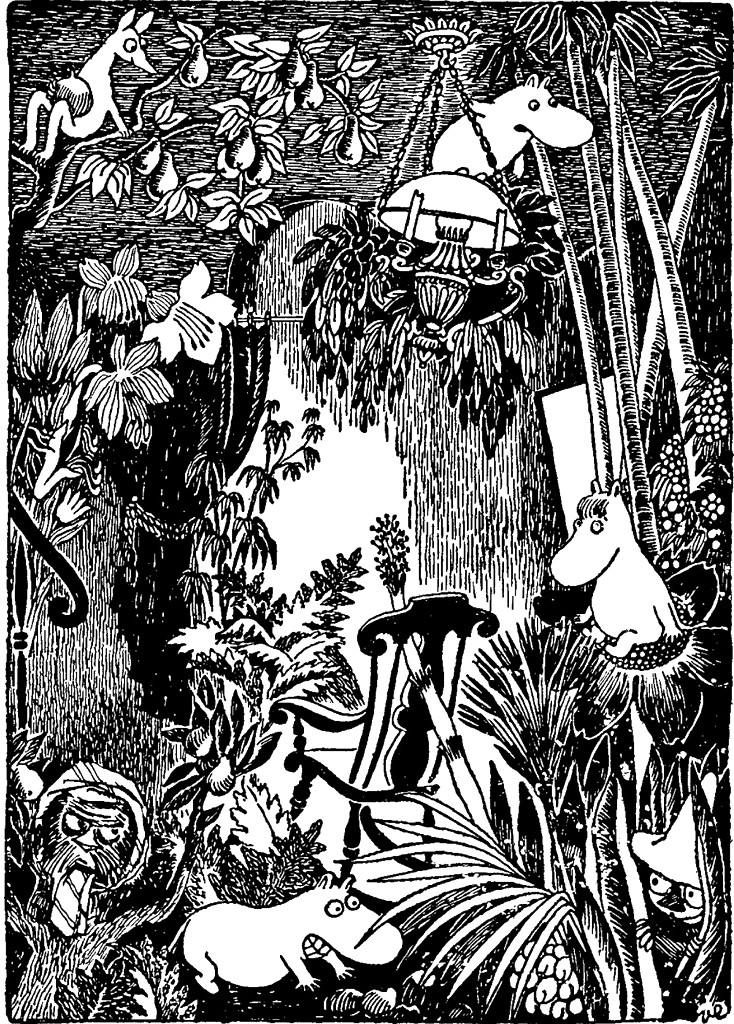
\includegraphics[width=450pt,height=631pt]{_27.jpg}
\caption{}
\label{_27}
\end{figure}

``Nu ja,'' diris la patrino de Mumintrolo. ``Sed ili ŝajne amuziĝas.''

``Ankaŭ mi,'' diris Muminpatro. ``Donu al mi bananon, mi petas.''

Tiel oni amuziĝis ĝis vespere. Neniu zorgis pri tio ke la kela pordo enkreskiĝis kaj neniu memoris la kompatindan hemulon.

Li ankoraŭ sidis kun la malseka robo pendante ĉirkaŭ la kruroj gardante la mamlukon. De temp' al tempo li manĝis pomon aŭ kalkulis la stamenojn de ĝangala floro, sed intertempe li plejparte suspiris.

Jam finis pluvi kaj la krepusko alvenis. Kaj en la sama momento kiam la suno subiris io okazis al la verda monteto ĉirkaŭ la mumindomo. Ĝi komencis velki, same rapide kiel ĝi elkreskis. La fruktoj ŝrumpis kaj falis teren. La floroj pendis kaj la folioj kunvolvis sin. Denove la domo pleniĝis de susurado kaj kraketado. La hemulo dum kelka tempo rigardis, poste li iris antaŭen kaj iomete tiris branĉon. Ĝi tuj rompiĝis kaj estis seka kiel tindro. Tiam la hemulo ekhavis ideon. Li kolektis enorman amason da branĉoj kaj branĉetoj, iris alporti alumetojn el la ŝtipobudo, kaj poste li ekbruligis krakantan fajregon meze de la ĝardena pado.

Kontenta kaj ĝoja la hemulo sidiĝis apud la fajro por sekigi sian robon.

Post kelka tempo li ekhavis alian ideon. Kun superhemulaj fortoj li trenis la voston de la mamluko en la fajron. Fritita fiŝo estis lia plej ŝatata manĝo.

\begin{figure}[htbp]
\centering
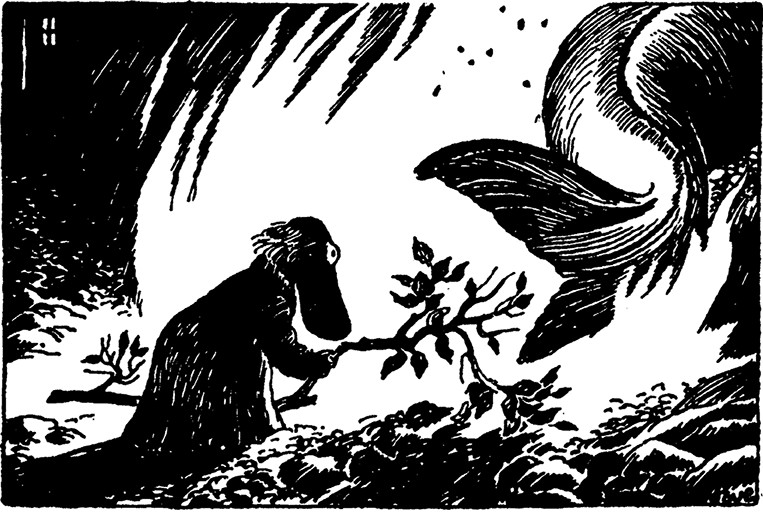
\includegraphics[width=450pt,height=299pt]{_28.jpg}
\caption{}
\label{_28}
\end{figure}

Tiel okazis ke kiam la muminfamilio kaj iliaj sovaĝaj amikoj batis al si vojon tra la verando kaj puŝmalfermis la pordon, ili ekvidis tre feliĉan hemulon kiu jam manĝis seponon de la mamluko.

``Vi fieraĉulo!'' diris la snorko. ``Nun mi neniam havis tempon pesi mian fiŝon!''

``Pesu min kaj adiciu'', proponis la hemulo kiu tiutage havis unu el siaj plej helaj tagoj.

``Nun ni bruligu la praarbaron!'' diris Muminpatro. Kaj ili elportis la tutan rubon el la domo kaj faris la plej grandan fajron iam viditan en Muminvalo.

La mamluko estis fritita sur ardoj en sia plena longo kaj manĝita ĝis la nazopinto. Sed dum longa tempo poste oni kverelis pri kiel longa ĝi estis; ĉu ĝi atingis de la ŝtuparo ĝis la ŝtipobudo aŭ nur ĝis la siringoj.

\chapter[Sesa Ĉapitro]{}


\begin{figure}[htbp]
\centering
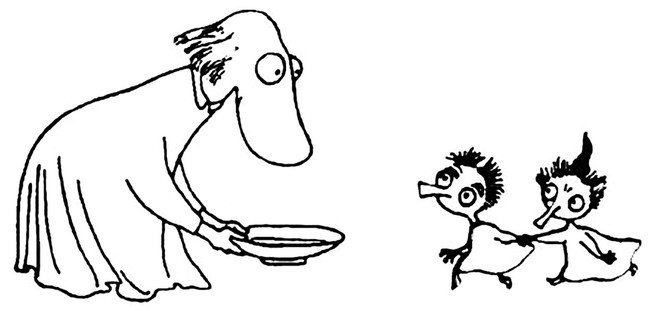
\includegraphics[width=395pt,height=189pt]{_29.jpg}
\caption{}
\label{_29}
\end{figure}

\begin{center}\textbf{\Large\color{ForestGreen}\textsc{Sesa Ĉapitro}}\end{center}

\noindent\textit{en kiu Tofslo kaj Vifslo eniras la historion, kunportante misteran valizon kaj persekutate de la morho, kaj en kiu la snorko gvidas juĝoproceson.}
\hfill \break
\hypertarget{Sesa Ĉapitro}{}
\label{Sesa Ĉapitro}


\noindent En iu frua mateno meze de aŭgusto Tofslo kaj Vifslo alvenis paŝante sur la monto, proksimume en la sama loko kie Snif trovis la ĉapelon de sorĉisto.

Ili haltis sur la pinto kaj rigardis suben al Muminvalo. Tofslo havis ruĝan ĉapon surkape kaj Vifslo portis grandan valizon. Ili venis tre longan vojon kaj estis sufiĉe lacaj. Sub iliaj piedoj inter betuloj kaj pomarboj matena fumo altiĝis el la kamentubo de la mumindomo.

``Jen fumslo,'' diris Vifslo.

``Oni kuirslas ion,'' diris Tofslo kapjesante. Poste ili ekiris suben en la valon interparolante en la mirinda maniero aparta de ĉiuj tofsloj kaj vifsloj. Ĉiuj ja ne komprenis ĝin, sed la ĉefa afero estis ke ili mem sciis pri kio temas.

``Ĉu vi penslas ke ni povos envensli?'' scivolis Tofslo.

``Tio dependslas,'' diris Vifslo. ``Ne ektimslu se oni malamikslas al ni.''

Tre singarde ili plandis ĝis la domo kaj timide haltis ĉe la ŝtuparo.

``Ĉu ni kuraĝslas frapsli?'' diris Tofslo. ``Imagu se iu elvenslas kaj krislas.''

Tiumomente la patrino de Mumintrolo eligis la kapon tra la fenestro kaj kriis: ``Kafon!''

Tofslo kaj Vifslo tiel terure ektimis ke ili ĵetis sin tra la luko de la terpoma kelo.

``Ej,'' diris Muminpatrino saltetante. ``Ŝajne du ratoj enŝteliĝis en la kelon. Snif, kuru suben kun iom da lakto por ili!''

Poste ŝi ekvidis la valizon kiu restis antaŭ la ŝtuparo. ``Kun pakaĵo,'' cerbumis la patrino. ``Nu ja. Do ili alvenas por resti.''

Kaj ŝi vagis for por trovi Muminpatron kaj peti lin fari du pliajn litojn. Sed tre, tre malgrandajn. Dume Tofslo kaj Vifslo enfosis sin inter la terpomojn tiel ke nur la okuloj vidiĝis, kaj tie ili en granda teruro atendis kio okazos al ili.

``Ĉiuokaze ili kuirslas kafslon,'' murmuris Vifslo.

``Iu venslas!'' flustris Tofslo. ``Silentslu kiel mitulslo!''

La kela pordo knaris kaj sur la plej supra ŝtupo staris Snif kun lanterno en unu mano kaj telero da lakto en la alia.

``Saluton! Kie vi estas?'' diris Snif.

Tofslo kaj Vifslo rampis eĉ pli suben kaj firme tenis unu la alian.

``Ĉu vi volas lakton?'' diris Snif iom pli laŭte.

``Li trompslas nin,'' flustris Vifslo.

``Se vi pensas ke mi intencas stari ĉi tie duonon de la tago vi eraras,'' diris Snif kolere. ``Malico aŭ stulto. Aĉaj stultaj ratoj kiuj ne havas prudenton iri tra la ĉefa pordo!''

Sed tiam Vifslo serioze malĝojis kaj diris: ``Ratslo vi mem povslas esti.''

``Nu, ĉu krome ili estas eksterlandanoj,'' diris Snif. ``Prefere mi venigu la patrinon de Mumintrolo ĉi tien.''

Li ŝlosis la kelan pordon kaj kuris en la kuirejon.

``Nu, ĉu ili volis lakton?'' demandis Muminpatrino.

``Ili parolas fremdlingve,'' diris Snif. ``Neniu povas kompreni kion ili diras!''

``Kiel tio sonis?'' demandis Mumintrolo kiu pistis kardamomon kun la hemulo.

``Ratslo vi mem povslas esti,'' diris Snif.

Muminpatrino suspiris. ``Ĉi tio estos bele, ŝi diris. Kiel mi komprenu kiun deserton ili deziras en sia naskiĝtago aŭ kiom da kusenoj ili volas havi subkape?''

``Ni devos lerni ilian lingvon,'' diris Mumintrolo. ``Tio sonas facile. Atslo, itslo, utslo.''

``Mi pensas ke mi komprenas ilin,'' diris la hemulo pripenseme. ``Kredeble ili diris al Snif ke li estas maljuna kalva rato.''

Snif ruĝiĝis kaj streĉis la nukon.

``Vi mem iru paroli kun ili, se vi estas tiel sagaca,'' li diris.

La hemulo paŝis ĝis la kela ŝtuparo kaj vokis amike: ``Bonvenslon, bonvenslon!''

Tofslo kaj Vifslo eligis la kapon el la terpomaro por rigardi lin.

``Laktslo! Bonsla!'' pluis la hemulo.

Tiam Tofslo kaj Vifslo plandis supren laŭ la ŝtuparo kaj eniris en la salonon.

Snif rigardis ilin kaj konstatis ke ili estas multe pli malgrandaj ol li mem. Tial li sentis sin pli amika kaj diris superece: ``Saluton. Plezure renkonti vin.''

``Dankslon, la samslon al vi!'' diris Tofslo.

``Ĉu vi kuirslas kafslon?'' scivolis Vifslo.

``Kion ili nun diris?'' demandis Muminpatrino.

``Ili malsatas,'' diris la hemulo. ``Sed ili ankoraŭ ne trovas la aspekton de Snif tre valora.''

``Do sciigu al ili,'' diris Snif indigne, ``ke mi neniam en la vivo vidis du tiajn haringovizaĝojn. Kaj nun mi iros eksteren.''

``Snifslo kolersla,'' diris la hemulo. ``Stultsla!''

``Mi petas enveni trinki kafon,'' diris la patrino de Mumintrolo nervoze.

Kaj ŝi montris al Tofslo kaj Vifslo la vojon al la verando dum la hemulo postsekvis, tre fiera pri sia nova rolo de interpretisto.
\sectionbreak

Tiel Tofslo kaj Vifslo estis inkluzivitaj en la mumindomanaron. Ili ne faris multe da bruo kaj plejparte ili rondiris man-en-mane. Kaj la valizon ili kunportis ĉie. Sed kiam krepuskis ili rimarkeble maltrankvilis kaj kuris supren-suben laŭ la ŝtuparoj kaj kaŝiĝis sub tapiŝo.

``Kiel vi fartslas?'' scivolis la hemulo.

``La morho venslas!'' flustris Vifslo.

``La morho? Kiu estas tiu?'' demandis la hemulo kaj iom ektimis.

Tofslo vastigis la okulojn, montris la dentojn kaj igis sin laŭeble granda.

``Kruelsla kaj terursla!'' diris Vifslo. ``Fermslu la pordslon al la morho!''

La hemulo kuris al Muminpatrino kaj diris: ``Ili asertas ke kruela kaj terura morho venos ĉi tien. Ni devas ŝlosi ĉiujn pordojn nokte!''

``Sed ni ja havas ŝlosilon nur al la kela pordo,'' diris la patrino de Mumintrolo maltrankvile. ``Tiel ĉiam estas pri eksterlandanoj.'' Kaj ŝi iris paroli kun Muminpatro pri la afero.

``Ni devos armi nin kaj movi la meblojn antaŭ la pordon,'' diris la patro de Mumintrolo. ``Tia terure granda morho povas esti danĝera. Mi metos alarmsonorilon en la salonon kaj Tofslo kaj Vifslo rajtos dormi sub mia lito.''

Sed Tofslo kaj Vifslo jam eniris komodan tirkeston kaj rifuzis elveni.

Muminpatro skuis la kapon kaj iris preni sian fusilon el la ŝtipobudo.

Jam estis aŭguste mallume eksterdome kaj la ĝardeno estis plena de velure nigraj ombroj. En la arbaro susuris malgaje, kaj la lampiroj eliris kun siaj poŝlampoj.

La patro ne povis eviti senti iom timige iri alporti la fusilon. Se tiu morho nun kuŝus malantaŭ arbedo! Oni ja eĉ ne sciis kiel ĝi aspektas.

Kaj antaŭ ĉio, kiel granda ĝi estas. Kiam Muminpatro revenis en la verandon li metis la sofon antaŭ la pordon kaj diris: ``La lampo devas lumi dum la tuta nokto! Ĉiu estu alarmpreta kaj Snufmumriko ĉi-nokte devas dormi endome.''

Estis terure ekscite. La patro de Mumintrolo frapetis al la komodkesto kaj diris: ``Ni protektos vin!''

Sed ĉio estis silenta en la kesto. Tiam la patro eltiris ĝin por vidi ĉu Tofslo kaj Vifslo jam estas forrabitaj. Sed ili dormis pace kaj apud si ili havis la valizon.

``Eble ni tamen iru enlitiĝi,'' li diris. ``Sed armu vin, ĉiuj!''

Dum granda timado kaj multe da parolado oni retiriĝis en siajn ĉambrojn kaj baldaŭ regis silento en la mumindomo. Nur la petrollampo brulis sola sur la salona tablo.

La horloĝo batis la dekduan horon. Ĝi batis la unuan. Iom post la dua vekiĝis la moskorato kaj sentis ke li devas iri suben. Li dormeme plandis en la verandon. Tie li en granda surpriziĝo restis staranta antaŭ la sofo. Ĝi staris antaŭ la pordo kaj ĝi estis peza. ``Kiaj ideoj,'' murmuris la moskorato kaj trenis la sofon plenforte. Kaj tiam kompreneble eksonoris la alarmsonorilo kiun la patro de Mumintrolo starigis.

En unu momento la domo pleniĝis de krioj, fusilpafoj kaj tretado de multaj piedoj. Ĉiuj kuris suben en la salonon kun hakiloj, tondiloj, ŝtonoj, fosiloj, tranĉiloj kaj rastiloj kaj haltis gapante al la moskorato.

``Kie estas la morho?'' kriis Mumintrolo.

``Ej, tio estas mi,'' diris la moskorato ĉagrenite. ``Mi nur volis iri eksteren por iomete pisi. Mi ja ne memoris vian stultan morhon.''

``Do eliru tuj,'' diris la snorko. ``Sed ne refaru tion! Kaj li vaste malfermis la verandan pordon.''

Tiam -- ili vidis la morhon. Ĉiu el ili vidis ŝin. Ŝi staris senmova sur la sablopado malsupre de la ŝtuparo gapante al ili per rondaj senesprimaj okuloj.

Ŝi ne estis tre granda nek aspektis tre danĝera. Oni nur sentis ke ŝi estas terure malica kaj povas atendi kiel ajn longe.

Kaj \emph{tio} estis terura.

\begin{figure}[htbp]
\centering
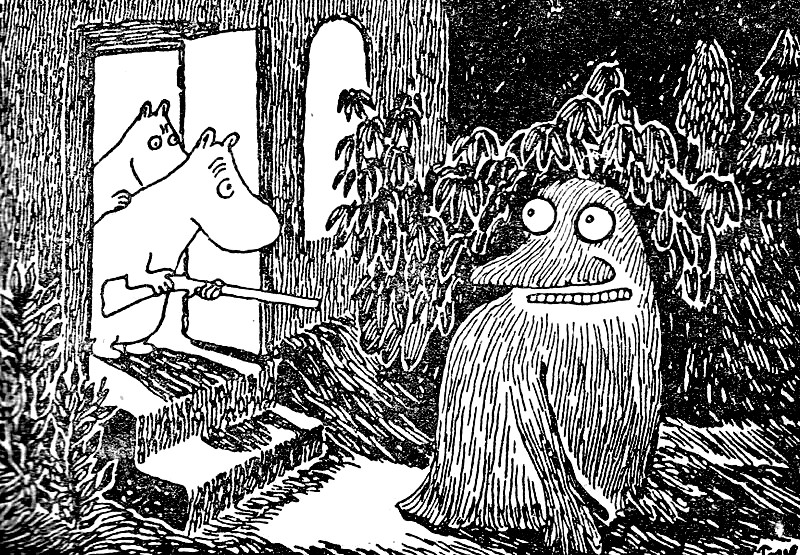
\includegraphics[width=449pt,height=313pt]{_30.jpg}
\caption{}
\label{_30}
\end{figure}

Neniu ekhavis la ideon ataki ŝin. Ŝi sidis dum kelka tempo, poste ŝi forglitis en la mallumon de la ĝardeno. Sed kie ŝi sidis la tero frostiĝis.

La snorko fermis la pordon kaj skuis sin. ``Kompatinda Tofslo kaj Vifslo,'' li diris. ``Hemulo, rigardu ĉu ili vekiĝis.''

Ili vekiĝis.

``Ĉu ĝi forirslis?'' demandis Vifslo.

``Dormslu trankvilsle,'' diris la hemulo.

Tofslo iom suspiris kaj diris: ``danksl' al Dislo!'' Kaj ili kuntrenis la valizon plej internen en la tirkeston por dormi plu.

``Ĉu oni do povas reendormiĝi?'' demandis Muminpatrino kaj demetis la hakilon.

``Faru tion,'' diris Mumintrolo. ``Snufmumriko kaj mi gardos vin ĝis la suno leviĝos. Sed por esti sekura metu vian mansakon sub la kusenon.''

Poste ili sidis solaj en la salono ludante pokeron ĝismatene. Kaj la morho ne plu vidiĝis tiunokte.
\sectionbreak
En la sekva mateno la hemulo maltrankvile venis en la kuirejon kaj diris: ``mi parolis kun Tofslo kaj Vifslo.''

``Nu, pri kio nun temas,'' demandis la patrino de Mumintrolo suspirante.

``Ilia valizo estas tio kion la morho deziras,'' diris la hemulo.

``Kia monstro!'' ekkriis la patrino. ``Forrabi de ili iliajn etajn posedaĵojn!''

``Jes, ĉu ne,'' diris la hemulo. ``Nun estas nur unu afero kiu komplikas la aferon. Ŝajnas ke ĝi estas la valizo de la morho.''

``Hm,'' diris Muminpatrino. ``Tio efektive malfaciligas la aferon. Ni parolu kun la snorko, li organizas ĉion tiel bone.''

La snorko tre interesiĝis. ``Tio estas miriga kazo,'' li diris. ``Ni devos aranĝi kunvenon. Ĉiuj kunvenu ĉe la siringoj je la tria horo por pritrakti la aferon.''

Estis varma kaj bela posttagmezo, plena de odoroj kaj abeloj. La ĝardeno estis bela kiel gefianĉiĝa bukedo en la saturitaj koloroj de malfrua somero.

La hamako de la moskorato estis streĉita inter la arbedoj kaj provizita per afiŝo kie legeblis: Akuzisto de la Morho. La snorko mem sidis atendante sur kesto kaj surmetis perukon el lignolano. Ĉiuj povis vidi ke li estas juĝisto. Vidalvide al li sidis Tofslo kaj Vifslo manĝante ĉerizojn malantaŭ tabulo kiu klare estis la fako de la akuzitoj.

``Mi deziras esti ilia akuzisto,'' diris Snif (kiu ne forgesis ke Tofslo kaj Vifslo nomis lin maljuna kalva rato).

``Tiuokaze mi estos ilia defendisto,'' diris la hemulo.

``Kaj mi?'' demandis Snorkfraŭlino.

``Vi estu la voĉo de l' popolo,'' diris ŝia frato. ``Muminfamilio atestos. Kiom koncernas Snufmumrikon, li povos fari notojn pri la juĝa proceso. Sed zorge!''

``Oni demandas sin kial la morho ne havas defendiston,'' diris Snif.

``Tio ne necesas,'' diris la snorko. ``La morho pravas. Ĉu vi pretas? Atentu. Ni komencas.''

Li trifoje batis al la kesto per martelo.

``Ĉu vi entutsle komprenslas?'' demandis Tofslo.

``Nenislon ajn,'' diris Vifslo kaj blovis ĉerizkernon sur la juĝiston.

\begin{figure}[htbp]
\centering
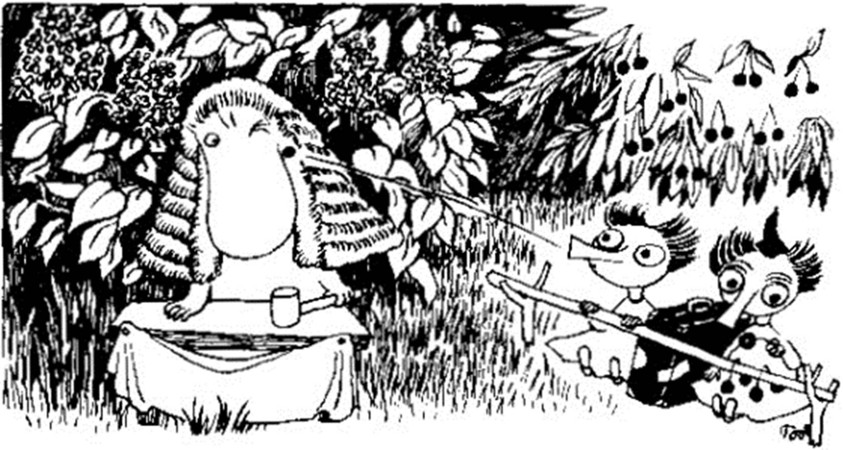
\includegraphics[width=450pt,height=240pt]{_31.jpg}
\caption{}
\label{_31}
\end{figure}

``Vi parolu nur kiam mi admonas,'' diris la snorko. ``Jes aŭ ne. Nenion kroman. Ĉu la koncerna valizo apartenas al vi aŭ al la morho?''

``Jesle!'' diris Tofslo.

``Nesle!'' diris Vifslo.

``Notu ke ili kontraŭdiras sin!'' kriis Snif.

``La snorko batis al la kesto. Trankvile!'' li vokis. ``Nun mi demandas lastfoje kies estas la valizo.''

``Nisla!'' diris Vifslo.

``Ili diras ke ĝi \emph{estas} ilia,'' tradukis la hemulo. ``Ĉi-matene ili diris male.''

``Nu, do ni ne bezonos doni ĝin al la morho,'' diris la snorko trankviliĝinte. ``Sed estas domaĝe pro ĉiuj miaj aranĝoj.''

Tofslo streĉis sin kaj flustris ion al la hemulo.

``Tofslo diras ĉi tiel,'' diris la hemulo. ``Nur la \emph{Enhavo} de la valizo apartenas al la morho.''

``Ha,'' diris Snif. ``Mi kredis tion. La afero estas klara sen io plua. La morho rericevos sian Enhavon kaj la haringovizaĝoj konservos sian malnovan valizon.''

``Tio tute ne estas klara!'' vokis la hemulo aŭdace. ``La demando ne estas kiu posedas la \emph{Enhavon}, sed kiu havas pli grandan \emph{rajton} je ĝi. Ĉio okazu leĝe kaj rajte! Vi ĉiuj vidis la morhon. Nun mi demandas vin, ĉu ŝi aspektis kvazaŭ ŝi rajtus je la Enhavo?''

``Vi pravas,'' diris Snif surprizite. ``Vi ja estas vere ruza! Sed pensu pri kiel sola la morho estas ĝuste ĉar neniu ŝatas ŝin kaj ŝi malŝatas ĉiujn. La Enhavo eble estas la sola afero kiun ŝi havas! Ĉu nun ankaŭ tio estu forprenita de ŝi? Sola kaj forpuŝita en la nokton,'' daŭrigis Snif per tremanta voĉo, ``prirabita je sia sola posedaĵo de tofsloj kaj vifsloj{\ldots}''

Li viŝis la nazon kaj ne povis daŭrigi.

La snorko frapis al la kesto. ``La morho ne bezonas defendan paroladon,'' li diris. ``Krome via vidpunkto estas emocia, kaj same tiu de la hemulo. Atestantoj antaŭen! Bonvolu atesti!''

``Ni tre ŝatas Tofslon kaj Vifslon,'' opiniis la muminfamilio. ``La morhon ni malŝatis jam dekomence. Estas malĝoje se ŝi devos rehavi sian Enhavon.''

``Necesas juĝi juste,'' diris la snorko solene. ``Vi devas esti aferecaj! Precipe ĉar Tofslo kaj Vifslo neniam vidas diferencon inter justo kaj maljusto. Ili naskiĝis tiaj kaj ne povas helpi tion. Akuzisto, kion vi volas aldoni?''

Sed la moskorato endormiĝis en la hamako.

``Nu,'' diris la snorko. ``Li sendube ne estis interesita. Ĉu ni jam diris ĉion kio estu dirita antaŭ ol mi eldiros la juĝon?''

``Pardonu,'' diris la voĉo de l' popolo, ``sed ĉu ne klariĝus se ni ekscius kio efektive estas la Enhavo?''

Tofslo denove ion flustris. La hemulo kapjesis. ``Ĝi estas sekreto,'' li diris. ``Tofslo kaj Vifslo trovas la Enhavon la plej bela afero ekzistanta, sed la morho nur trovas ĝin la plej valora.''

La snorko plurfoje kapjesis kaj ĉifis sian frunton. ``Ĝi estas malfacila kazo,'' li diris. ``Tofslo kaj Vifslo rezonis tute prave, tamen ili agis maljuste. Kaj necesas juĝi juste. Mi devas pensi. Nun silentu, ĉiuj.''

Tute kvietiĝis inter la siringoj. Abeloj zumis, la ĝardeno brulis en la sunbrilo.

Subite malvarma trablovo trairis la herbejon. La suno kaŝiĝis de nuboj kaj la ĝardeno ŝajnis griza.

``Kio estis tio?'' diris Snufmumriko levante la skribilon de la protokolo.

``Ŝi revenis,'' flustris Snorkfraŭlino.

Sur la frosta herbejo la morho sidis gapante al ili.

Ŝi malrapide movis la rigardon al Tofslo kaj Vifslo. Ŝi komencis grumbli kaj malrapide trenis sin pli proksimen.

``Helpslu!'' kriis Tofslo. ``Savslu nin!''

``Haltu, morho,'' diris la snorko. ``Mi havas ion por diri al vi!''

La morho haltis.

``Mi finpensis,'' daŭrigis la snorko. ``Ĉu vi akceptas ke Tofslo kaj Vifslo rajtos aĉeti la Enhavon de la valizo? Kiu estos via prezo?''

``Alta!'' diris la morho kun glacia voĉo.

``Ĉu sufiĉas mia ora monto sur la insulo de hatifnatoj?'' demandis la snorko.

La morho kapneis.

``Hu, kiel malvarme estas ĉi tie,'' diris la patrino de Mumintrolo. ``Mi eniros preni ŝalon.'' Ŝi kuris tra la ĝardeno kie frosto sekvis la spuron de la morho kaj supren en la verandon.

Kaj tie Muminpatrino ekhavis ideon. Varmega pro feliĉo ŝi levis la ĉapelon de sorĉisto. Ke la morho ŝatu ĝin! Kiam la patrino revenis al la juĝa proceso ŝi metis la ĉapelon sur la herbojn kaj diris: ``Jen la plej valora aĵo en tuta Muminvalo! Ĉu vi scias kio kreskis el ĉi tiu ĉapelo? La plej belaj stireblaj nuboj, magia akvo kaj fruktarboj! La sola sorĉa ĉapelo de la mondo!''

``Pruvu!'' diris la morho malestime.

Tiam Muminpatrino metis kelkajn ĉerizojn en la ĉapelon. Ĉiuj atendis en tomba silento.

``Ke nur ne fariĝu io abomena el ili,'' flustris Snufmumriko al la hemulo.

Sed ili havis bonŝancon. Kiam la morho rigardis suben en la ĉapelon kuŝis tie manpleno da ruĝaj rubenoj.

``Jen vidu!'' diris Muminpatrino ĝoje. ``Kaj imagu kio estos se oni ekzemple enmetos kukurbon!''

La morho rigardis la ĉapelon. Ŝi rigardis Tofslon kaj Vifslon. Refoje ŝi rigardis la ĉapelon. Oni vidis ŝin pensi plenforte.

Fine la morho kaptis la ĉapelon de sorĉisto kaj sen unu vorto forglitis kiel grize malvarma ombro. Jen la lasta fojo kiam ŝi vidiĝis en Muminvalo, kaj la lasta fojo kiam oni vidis la ĉapelon de sorĉisto.

Subite la koloroj refariĝis varmaj kaj la somero daŭris, zuma kaj odora.

``Dank' al Dio ke ni liberiĝis de tiu ĉapelo,'' diris Muminpatrino. ``Nun ĝi esceptokaze kaŭzis ion prudentan.''

``Sed niaj nuboj \emph{estis} amuzaj,'' diris Snif.

``Kaj ludi Tarzan en la praarbaro,'' diris Mumintrolo melankolie.

``Kiel bonsle tio irslis!'' diris Vifslo gaje kaj levis la valizon, kiu dum la tuta tempo staris en la fako de akuzitoj.

``Mirindsle,'' diris Tofslo prenante la manon de Vifslo. Kaj kune ili reiris ĝis la mumindomo dum la aliaj rigardis post ili.

``Kion ili nun diris?'' demandis Snif.

``Ĝis revido, proksimume,'' diris la hemulo.

\chapter[Lasta Ĉapitro]{}


\begin{figure}[htbp]
\centering
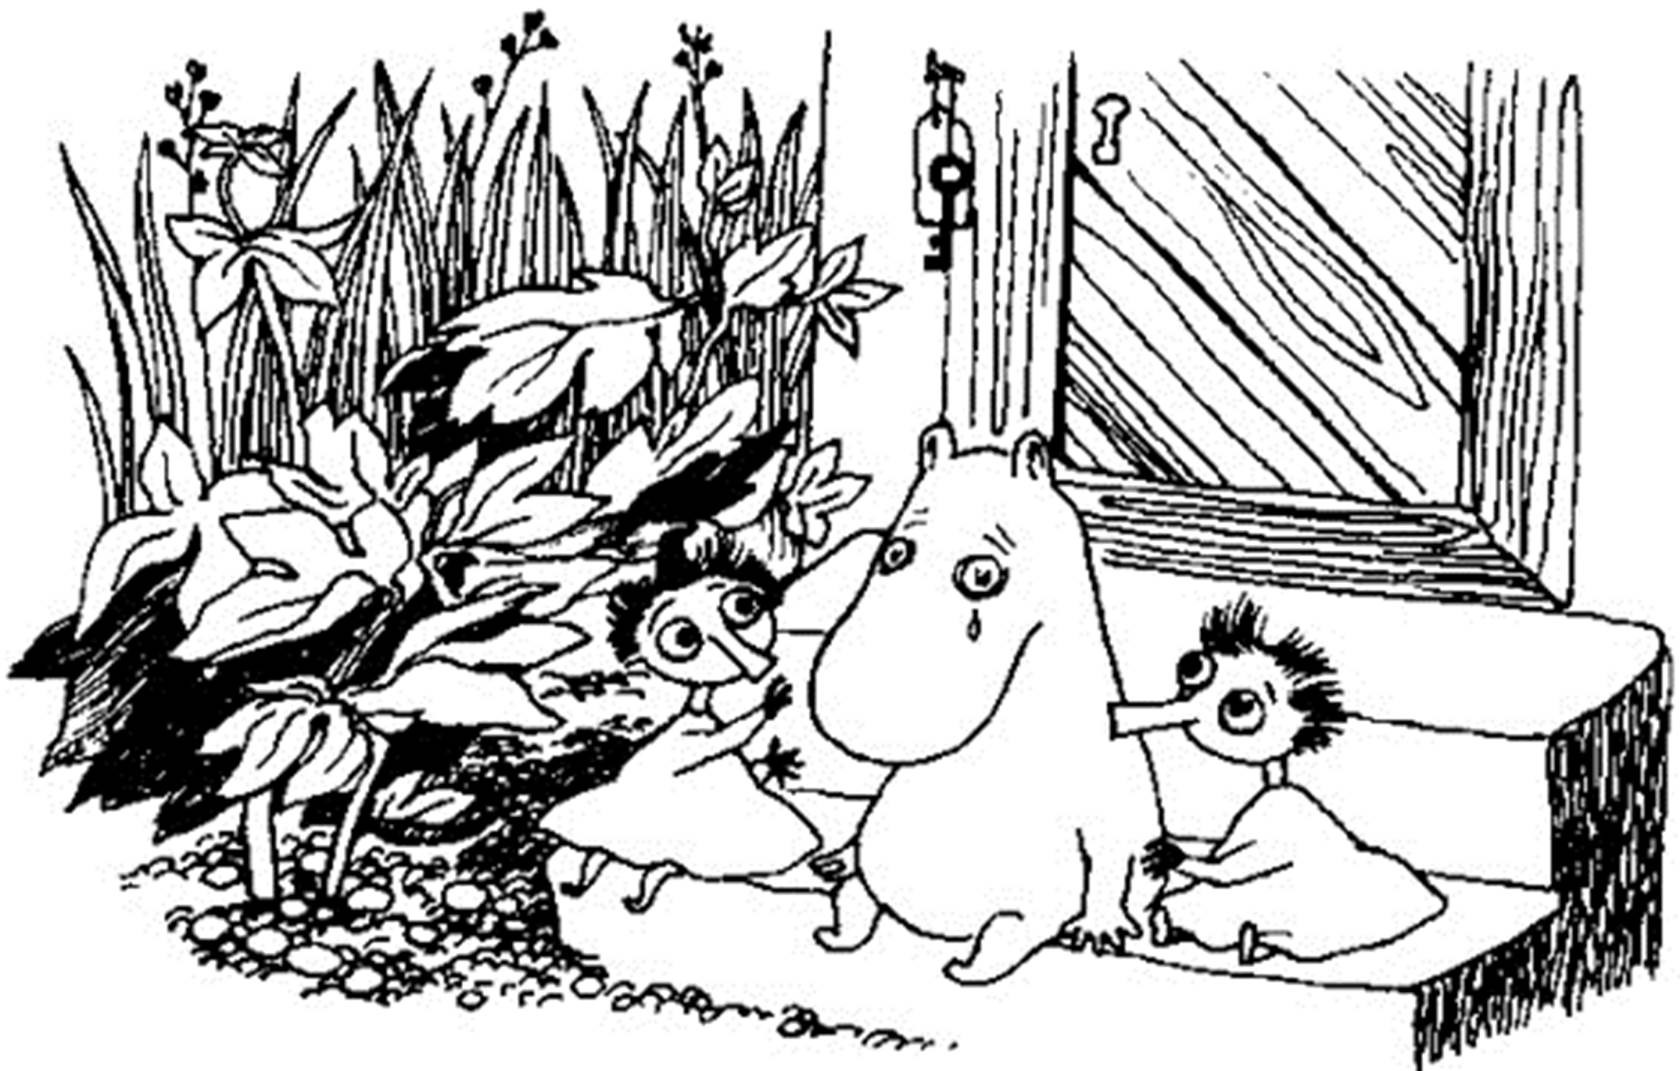
\includegraphics[width=450pt,height=286pt]{_32.jpg}
\caption{}
\label{_32}
\end{figure}

\begin{center}\textbf{\Large\color{ForestGreen}\textsc{Lasta Ĉapitro}}\end{center}

\noindent\textit{kiu estas tre longa kaj priskribas la foriron de Snufmumriko kaj kiel la mistera valiza enhavo estis malkaŝita, krome kiel la patrino de Mumintrolo rericevis sian mansakon kaj pro ĝojo aranĝis grandan festenon, kaj fine kiel la sorĉisto alvenis en Muminvalon.}
\hfill \break
\hypertarget{Lasta Ĉapitro}{}
\label{Lasta Ĉapitro}


\noindent Estis en la fino de aŭgusto. Nokte strigoj blekis kaj vespertoj en grandaj nigraj aroj alvenis rondiri sensone super la ĝardeno. La arbaro estis plena de fajreroj kaj la maro estis malkvieta. Troviĝis atendo kaj malĝojo en la aero, kaj la luno iĝis granda kaj varmkolora. Mumintrolo ĉiam plej multe ŝatis la plej lastajn somerajn semajnojn, sed li ne sciis precize kial.

La tono de vento kaj maro estis alia, ĉio odoris je ŝanĝo, la arboj staris atendante.

`Mi demandas min ĉu ne okazos io nekutima,' pensis Mumintrolo.

Li vekiĝis kaj kuŝis rigardante en la plafonon. Devas esti fruege matene kaj estos sunbrilo, li plu cerbumis.

Poste li turnis la kapon kaj vidis ke la lito de Snufmumriko estas malplena.

Kaj tiumomente li aŭdis la sekretan signalon sub la fenestro, unu longan fajfon kaj du mallongajn, kio signifas: ``Kaj kiajn planojn vi havas hodiaŭ?''

Mumintrolo saltis el la lito kaj rigardis eksteren. La ĝardeno ankoraŭ kuŝis en ombro kaj estis nevarme. Kaj jen staris Snufmumriko atendante.

``Hej ho,'' vokis Mumintrolo, sed tre mallaŭte por veki neniun, kaj poste li grimpis suben laŭ la ŝnura ŝtupetaro.

``Saluton,'' li diris.

``Saluton al vi,'' diris Snufmumriko.

Ili vagis ĝis la rivero kaj sidiĝis sur la pontan apogilon kun la kruroj pendante super la akvo. La suno nun atingis super la arbopintojn kaj lumis en iliajn vizaĝojn.

``Ĝuste ĉi tiel ni sidis ĉi-printempe,'' diris Mumintrolo. ``Ni ĵus vekiĝis el la vintrodormo, kaj estis la unua tago. Ĉiuj aliaj ankoraŭ dormis.''

Snufmumriko kapjesis. Li faradis kanoboatojn kiujn li lasis veli malsupren sur la rivero.

``Kien ili iros?'' demandis Mumintrolo.

``Al lokoj kie mi ne estas,'' diris Snufmumriko. Unu boato post alia turniĝis ĉirkaŭ la riverkurbiĝo kaj malaperis.

``Ŝarĝitaj per cinamo, ŝarkodentoj kaj smeraldoj,'' diris Mumintrolo.

Snufmumriko suspiris.

``Vi parolis pri planoj?'' diris Mumintrolo. ``Ĉu vi mem havas iun?''

``Jes,'' diris Snufmumriko. ``Mi havas planon. Sed ĝi estas unu el la solecaj, vi scias.''

Mumintrolo tre longe rigardis lin. Poste li diris: ``Vi intencas foriri.''

Snufmumriko kapjesis.

Ili sidis kelkan tempon svingante la krurojn super la rivero ne parolante. Ĝi fluis plu kaj plu sub ili, senĉese, ĝis la fremdaj lokoj kien Snufmumriko sopiris kaj iros tute sola.

``Kiam vi iros?'' demandis Mumintrolo.

``Nun tuj!'' diris Snufmumriko kaj ĵetis ĉiujn kanoboatojn en la akvon samtempe. Li saltis de la ponta apogilo kaj flaris en la matena aero. Estis bona tago por vagado. La monta kresto ruĝis en la sunbrilo kaj la vojo serpentis supren al ĝi kaj malaperis transen. Tie troviĝis alia valo, kaj poste sekvis aliaj montoj{\ldots}

Mumintrolo rigardis dum Snufmumriko pakis la tendon.

``Ĉu vi longe restos fore?'' li demandis.

``Ne,'' diris Snufmumriko. ``En la unua printempa tago mi ree estos ĉi tie kaj fajfos sub la fenestro. Unu jaro rapidege pasas!''

``Jes,'' diris Mumintrolo. ``Ĝis tiam.''

``Ĝis la,'' diris Snufmumriko.

Mumintrolo restis surponte. Li vidis Snufmumrikon pli kaj pli malgrandiĝi kaj poste malaperi inter betuloj kaj pomarboj. Sed post iom li aŭdis la buŝharmonikon. Snufmumriko ludis `\emph{Ĉiuj bestetoj bantigas la voston}'.

``Nun li ĝojas,'' diris Mumintrolo.

La muziko pli kaj pli mallaŭtiĝis kaj fine estis tute silente. Tiam Mumintrolo plandis reen tra la rose malseka ĝardeno.

Sur la ŝtuparo li trovis Tofslon kaj Vifslon kiu kaŭris kune en la sunbrilo.

``Salutslon,'' diris Tofslo.

``Saluton al vi,'' diris Mumintrolo, ĉar nun li jam lernis kompreni ilian lingvon (kvankam li parolis ĝin kun malfacilo).

``Ĉu vi plorslis?'' demandis Vifslo.

``Ej,'' diris Mumintrolo. ``Snufmumriko foriris.''

``Mi bedaŭrslas,'' diris Tofslo kompate. ``Ĉu povslas ĝojigsli vin iomete se vi rajtslos kisli Tofslon sur la nazlo?''

Mumintrolo kisis Tofslon amike sur la nazo, tamen li ne aspektis pli gaje.

Tiam Tofslo kaj Vifslo kunigis la kapojn kaj longe flustradis.

Poste Vifslo solene diris: ``Ni decidslis montri al vi la Enhavslon.''

``De la valizo?'' demandis Mumintrolo.

Tofslo kaj Vifslo fervore kapjesis. ``Venslu, venslu,'' ili diris kaj eniris sub la heĝojn.

Mumintrolo rampis post ili. En la plej densa arbedo li trovis sekretan lokon kie Tofslo kaj Vifslo ornamis la teron per lanugoj kaj pendigis konkojn kaj blankajn ŝtonetojn inter la branĉoj. Estis tute mallume tie ene. Neniu kiu preteriris la heĝon povus imagi ke tie troviĝas sekreta loko. Sur mato el basto staris la valizo de Tofslo kaj Vifslo.

``Tio estas la mato de Snorkfraŭlino,'' diris Mumintrolo. ``Ŝi serĉis ĝin hieraŭ.''

``Jesle,'' diris Vifslo. ``Ŝi tutsle ne povslis scii ke ni trovslis ĝin!''

``Hm,'' diris Mumintrolo. ``Kaj nun vi intencas montri al mi kion vi havas en via valizo?''

Tofslo kaj Vifslo feliĉe kapjesis. Ili stariĝis ambaŭflanke de la valizo kaj serioze kalkulis: ``Unusle! Dusle! trisle! Kaj jen ili malfermis la kovrilon kun klako.''

``Jen la plej mirinda{\ldots}'' diris Mumintrolo.

La tuta eta ejo pleniĝis de milda, ruĝa lumo. Antaŭ li kuŝis rubeno, granda kiel la kapo de pantero, arda kiel la sunsubiro, viva kiel fajro kaj akvobrilo.

``Ĉu vi ŝatslas ĝin?'' demandis Tofslo.

``Jes,'' diris Mumintrolo per malforta voĉo.

``Nun vi ne plu plorslos?'' diris Vifslo.

Mumintrolo kapneis.

\begin{figure}[htbp]
\centering
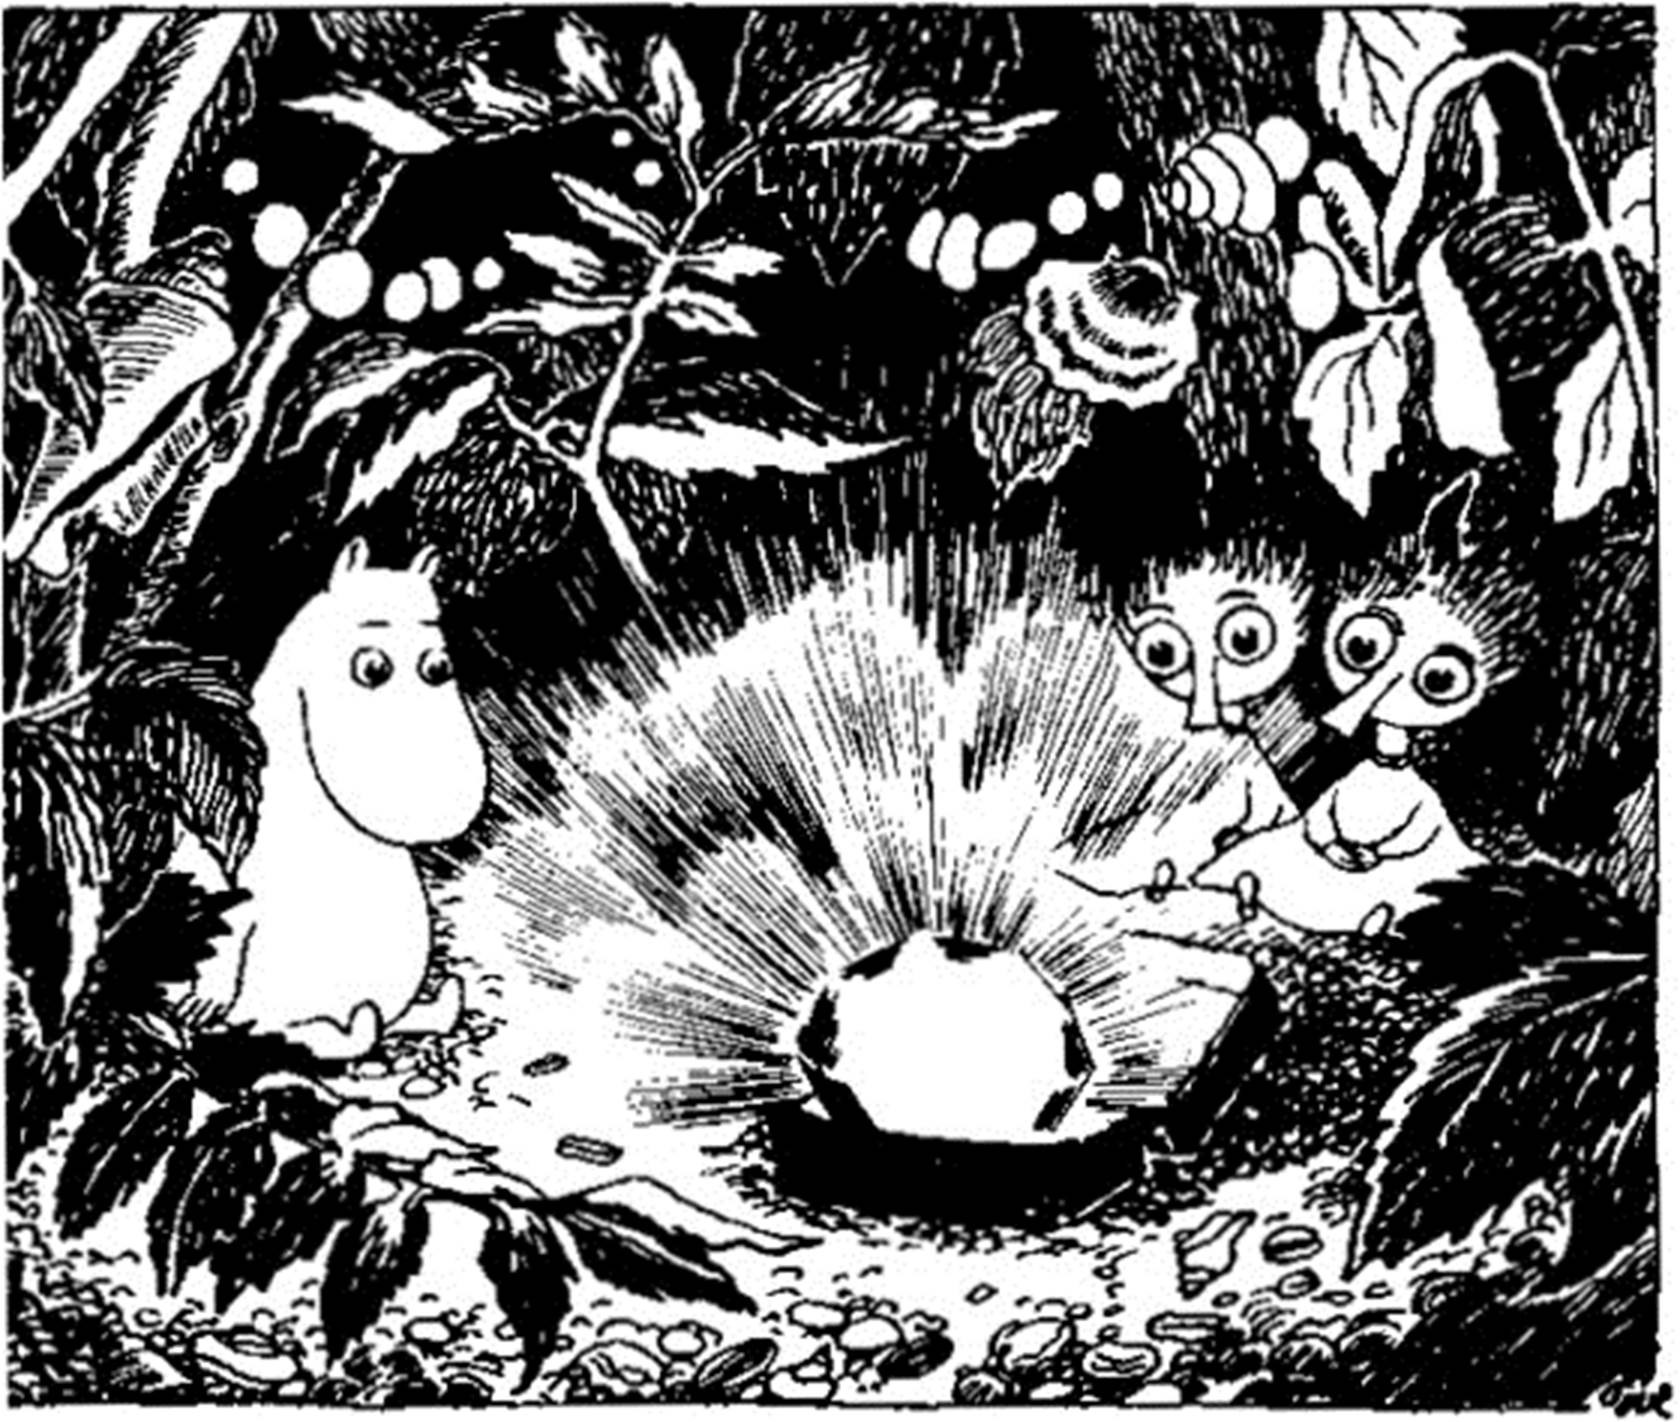
\includegraphics[width=499pt,height=423pt]{_33.jpg}
\caption{}
\label{_33}
\end{figure}

Tofslo kaj Vifslo kontente suspiris kaj sidiĝis por rigardi la gemon. Ili silente kaj ravite gapis en ĝin.

La rubeno ŝanĝiĝis kiel la maro. Jen ĝi estis nur hela, jen roza koloro flugis al ĝi, precize kiel sur neĝkovrita montopinto kiam la suno leviĝas -- kaj subite malhelruĝaj flamoj altiĝis el ĝia interno. Ĝi povis iĝi kvazaŭ nigra tulipo kun stamenoj el fajreretoj.

``Ho, se Snufmumriko povus vidi ĝin!'' diris Mumintrolo. Li staris tie longe, longege. La tempo iĝis tre malrapida kaj liaj pensoj grandegaj.

Fine li diris: ``Ĝi estas bela. Ĉu mi rajtos iam reveni rigardi ĝin?''

Sed Tofslo kaj Vifslo ne respondis.

Tiam Mumintrolo reelrampis el la heĝo, kaj li sentis iom da kapturniĝo en la pala taglumo kaj devis dum kelka tempo sidi sur la herbejo por ripozi.

`Jen la plej mirinda,' li pensis. `Mi povas mordi al mi la voston je tio ke ĝi estas la Reĝa Rubeno kiun la sorĉisto serĉas surlune. Imagu ke tiuj etaj Tofslo kaj Vifslo havas ĝin en sia valizo jam dekomence!' Mumintrolo profundiĝis en cerbumadon. Li ne rimarkis ke Snorkfraŭlino alvenis vagante tra la ĝardeno kaj sidiĝis apud lin. Post iom ŝi singarde palpis lian vostopenikon.

``Ho, ĉu estas vi!'' diris Mumintrolo saltetante. Snorkfraŭlino ridetis. ``Ĉu vi vidis mian novan frizaĵon?'' ŝi demandis turnante la kapon.

``Ehe,'' diris Mumintrolo.

``Vi pensas pri io alia,'' diris la snorkfratino. ``Ekzemple kio?''

``Mia matena rozo, tion mi ne povas rakonti,'' diris Mumintrolo. ``Sed mia koro pezas en mi, ĉar Snufmumriko forvojaĝis.''

``Ĉu vi certas?'' diris Snorkfraŭlino.

``Jes. Sed li unue diris ĝis revido al mi. Li vekis neniun alian ol min por diri ĝis revido,'' diris Mumintrolo.

Ili restis sur la herboj sentante la sunon altiĝi kaj varmigi. Snif kaj la snorko elvenis sur la ŝtuparon.

``Hola,'' diris Snorkfraŭlino. ``Ĉu vi scias ke Snufmumriko vojaĝis suden?''

``Sen mi!'' diris Snif indigne.

``Kelkfoje necesas esti sola,'' diris Mumintrolo. ``Vi ankoraŭ estas tro malgranda por kompreni tion. Kie estas la aliaj?''

``La hemulo iris kolekti fungojn,'' diris la snorko. ``Kaj la moskorato endomigis sian hamakon ĉar li trovas ke la noktoj komencas malvarmiĝi. Cetere via panjo hodiaŭ estas je tre malbona humoro!''

``Ĉu kolera aŭ malĝoja?'' demandis Mumintrolo surprizite.

``Plejparte malĝoja, mi pensas,'' diris la snorko.

``Do mi devas tuj eniri,'' diris Mumintrolo kaj stariĝis. ``Tio ja estas terura.''

Muminpatrino sidis sur la salona sofo kun malfeliĉa mieno.

``Kio nun?'' diris Mumintrolo.

``Kara infano, okazis io terura,'' diris lia patrino. ``Mia mansako malaperis. Mi ne elturniĝos sen ĝi! Mi serĉis ĉie sed ĝi ne troviĝas!''

``Kiel terure,'' diris Mumintrolo. ``Ni devos trovi ĝin por vi!''

Fariĝis grandega serĉado. Nur la moskorato rifuzis partopreni. El ĉio nenecesa, li diris, mansako estas la plej nenecesa. Pripensu. La tempo pasas kaj la tagoj ŝanĝiĝas tute egale ĉu la muminsinjorino estas kun mansako aŭ sen.

``Estas neimagebla diferenco,'' diris Muminpatro. ``Mi sentas la patrinon de Mumintrolo tute fremda se ŝi estas sen mansako. Mi neniam antaŭe vidis ŝin sen ĝi!''

``Ĉu estis multo en ĝi?'' demandis la snorko.

``Ne,'' diris Muminpatrino. ``Nur aĵoj kiuj povas esti bezonataj subite. Sekaj ŝtrumpoj, bombonoj, drato kaj stomakpulvoro kaj similaĵoj.''

``Kian premion ni ricevos se ni trovos ĝin?'' demandis Snif.

``Ion ajn!'' diris la patrino. ``Mi faros grandan festenon por vi kaj vi ricevos nur desertojn por tagmanĝo kaj neniu devos lavi sin aŭ enlitiĝi frue!''

Tiam la serĉado daŭris per duobla forto. Ili traserĉis la tutan domon.

Ili rigardis sub tapiŝoj kaj en litoj, en la forno kaj kelo, sub-kaj surtegmente. Ili serĉis en la tuta ĝardeno, en la ŝtipejo kaj malsupre ĉe la rivero. Neniu mansako.

``Vi ja ne grimpis sur arbojn kun ĝi aŭ kunportis ĝin kiam vi banis vin?'' demandis Snif.

``Ne,'' diris Muminpatrino. ``Ho, kiel malfeliĉa mi estas!''

``Ni dissendos telegramfoliojn!'' proponis la snorko.

Tion ili faris, kaj la telegramfolioj aperis tuj kun du grandegaj novaĵoj.

Snufmumriko Forlasas Muminvalon

estis skribite. \emph{Mistera forvojaĝo en la tagiĝo}! kaj per pli grandaj literoj:

La Mansako De Muminpatrino Malaperis!

\emph{Neniuj indikoj! Serĉado daŭras. Neimagebla aŭgusta festeno kiel retrova premio!}

Tuj kiam la novaĵo disvastiĝis estis granda svarmado en la arbaro, surmonte, ĉemare. Ĉiu simpla arbara rato ekiris por serĉi. Nur maljunuloj kaj kadukuloj restis hejme, kaj en tuta Muminvalo eĥiĝis vokado kaj kurado.

``Nu ja,'' diris la patrino de Mumintrolo. ``Kian bruon mi kaŭzis! Sed ŝi estis sufiĉe kontenta.''

``Kion ili serĉslas?'' demandis Vifslo.

``Mian sakon, kompreneble,'' diris Muminpatrino.

``Ĉu vian nigrslan?'' demandis Tofslo. ``Kun kvar poŝetsloj kaj en kislu eblas spegulsli sin?''

``Kion vi diris?'' demandis Muminpatrino. Ŝi estis tro maltrankvila por povi koncentriĝi.

``La nigrsla kun kvar poŝsloj,'' diris Tofslo.

``Jes jes,'' diris la patrino. ``Eliru ludi, amiketoj, kaj ne zorgu pri mi!''

``Kion vi penslas?'' demandis Vifslo kiam ili venis en la ĝardenon.

``Mi ne povslas vidi ŝin tiel malĝojsli,'' diris Tofslo.

``Do ŝi ja devos ricevsli ĝin,'' diris Vifslo suspirante. ``Sed estis bonsle dormsli en la poŝetsloj.''

Do Tofslo kaj Vifslo iris en sian sekretan lokon kiun ankoraŭ neniu trovis kaj eltiris la mansakon de Muminpatrino el sub la rozobranĉoj.

Estis precize la dekdua horo kiam Tofslo kaj Vifslo iris tra la ĝardeno trenante la sakon inter si. La akcipitro tuj ekvidis ilin kaj disvokis la novaĵon super Muminvalo. Novaj telegramfolioj estis dissendataj ĉien: MANSAKO DE MUMINPATRINO TROVITA! \emph{Tofslo kaj Vifslo trovis ĝin! Kortuŝaj scenoj en mumindomo!}

``Ĉu efektive estas vere?'' ekkriis la patrino de Mumintrolo. ``Ho, kiel ege bone! Kie vi trovis ĝin?''

``Sub la arbedsloj,'' diris Tofslo. ``Estis tiel bonsle dormsli en{\ldots}''

Sed tiumomente la gratulantoj enkuris tra la pordo kaj la patrino neniam eksciis ke ilia mansako estis uzata kiel dormejo de Tofslo kaj Vifslo (kaj tio eble estis same bona).

Cetere neniu povis pensi pri io ajn alia ol la granda aŭgusta festeno.

Ĉio devis pretiĝi antaŭ ol la luno leviĝos. Imagu prepari grandan festenon kaj scii ke ĝi estos amuza kaj ke ĉiuj ĝustaj personoj partoprenos!

Eĉ la moskorato alvenis interesiĝante. Vi havu multajn tablojn, li diris. Tabletojn kaj tablegojn. En surprizaj lokoj. Neniu volas sidi senmova samloke en granda festeno. Ili kurados tien-reen pli aĉe ol kutime, mi timas. Kaj unue vi regalu per la plej bona kion vi havas.

Poste ne gravas kion ili ricevos ĉar tiam ili ĉiuokaze estos gajaj. Kaj ne ĝenu ilin per spektaklo, kantado kaj tiaĵoj, sed lasu ilin mem esti programo.

Kiam la moskorato eldiris tiun surprizan vivosaĝon li retiriĝis al sia hamako por legi en la libro pri la Neneceso de Ĉio.

``Kion mi surmetu?'' demandis Snorkfraŭlino nervoze. ``Ĉu la bluan harornamon el plumo aŭ la perlan diademon?''

``Prenu la plumojn,'' diris Mumintrolo. ``Nur plumoj ĉirkaŭ la oreloj kaj piedartikoj. Eventuale du-tri ŝovitaj en la vostopenikon.''

``Dankon!'' diris Snorkfraŭlino kaj ekkuris. En la pordo ŝi kunpuŝiĝis kun la snorko kiu alportis buntajn paperlanternojn.

``Atentu!'' li diris. ``Vi kaĉigas la lanternojn! Se mi povus kompreni por kio fratinoj utilas!'' Kaj li marŝis en la ĝardenon kaj komencis pendigi la lanternojn de arboj. Dume la hemulo aranĝis artfajraĵojn en konvenaj lokoj. Troviĝis blua stelpluvo, fajroserpentoj, bengala neĝoŝtormo, arĝentaj fontanoj kaj raketoj kun pafoj.

``Mi estas en tia neeltenebla ekscitiĝo!'' diris la hemulo. ``Ĉu ni ne povus sendi unu solan prove?''

``Ili ne vidiĝas en taglumo,'' diris la patro de Mumintrolo. ``Sed prenu fajroserpenton se vi volas kaj ekbruligu ĝin en la terpoma kelo.''

Muminpatro staris antaŭ la ŝtuparo preparante ruĝan vinpunĉon en kelkaj bareloj. Li aldonis al ĝi sekvinberojn kaj migdalojn, konfititan lotuson, zingibron, sukeron kaj muskatfloron, unu-du citronojn kaj kelkajn litrojn da sorpa likvoro por gustigi la tuton.

De temp' al tempo li gustumis la rezulton.

La rezulto estis bonega.

``Unu afero estas malĝojiga,'' diris Snif. ``Ni ne havos muzikon. Snufmumriko foriris.''

``Ni laŭtigos nian malnovan muzikskatolon,'' diris Muminpatro. ``Ĉio estos en ordo! La duan toston ni faros je la honoro de Snufmumriko.''

``Kies estos la unua?'' demandis Snif esperplene.

``De Tofslo kaj Vifslo, kompreneble,'' diris la patro.

La preparoj nur pliampleksiĝis. La loĝantoj de la tuta valo kaj arbaro, montaro kaj strando alportis manĝaĵojn kaj trinkaĵojn kaj ĉio estis metata sur la tablojn en la ĝardeno. Grandaj amasoj da lumaj fruktoj kaj enormaj buterpanpladoj, kaj sur tre malgrandaj tabloj sub la arbedoj oni prezentis nuksojn kaj folibukedojn, berojn sur tigoj, sukerradikojn kaj tritikajn spikojn. La patrino de Mumintrolo miksis patkukan paston en la bankuvo ĉar la potoj ne sufiĉis. Poste ŝi alportis dek unu netuŝitajn kruĉojn da konfitaĵo el la kelo (la dekdua bedaŭrinde krevis kiam la hemulo ekbruligis fajroserpentojn, sed tio ne gravis ĉar Tofslo kaj Vifslo lekis la plej grandan parton).

``Imagslu!'' diris Tofslo. ``Tiom da bruslo nur je nia honorslo!''

``Jes, ne facilslas komprensli tion,'' diris Vifslo.

Tofslo kaj Vifslo havis la honorajn lokojn ĉe la plej granda tablo.

Kiam jam tiel mallumiĝis ke eblis eklumigi la lanternojn, la hemulo albatis gongon kio signifis: Nun ni eku!

Unue estis tre solene.

Ĉiuj vestis sin kiel eble plej bele kaj sentis sin iom nenaturaj. Oni salutis kaj riverencis kaj diris: bone ke ne venis pluvo kaj imagu ke la mansako estis trovita.

Neniu kuraĝis sidiĝi.

Muminpatro faris enkondukan paroladeton en kiu li rakontis kial oni aranĝis ĉi tiun festenon kaj dankis Tofslon kaj Vifslon.

Poste la patro diris ion pri la mallonga norda somero kaj ke ĉiuj kiel eble plej ĝoju kaj poste li ekparolis pri kiel estis en lia junaĝo.

Tiam la patrino de Mumintrolo alveturigis tutan ĉarumon da patkukoj kaj ĉiuj ekaplaŭdis.

Tuj estis iom malpli solene kaj post iom la festeno estis en plena plenumo. La tuta ĝardeno, eĉ la tuta valo estis plena de lumigataj tabletoj. Lumo-muŝoj kaj lampiroj ekbrilis kiel fajreroj kaj la lanternoj enarbe balanciĝis pro la nokta vento el nordo kvazaŭ grandaj belaj fruktoj.

La raketo kun pafoj ekflugis al la aŭgusta ĉielo en bela arko, kaj altege ĝi eksplodis en pluvon el blankaj steloj kiuj malrapidege sinkis super la valo. Ĉiu besteto turnis la vizaĝon al la stelpluvo kaj hurais -- ho, estis mirinde!

\begin{figure}[htbp]
\centering
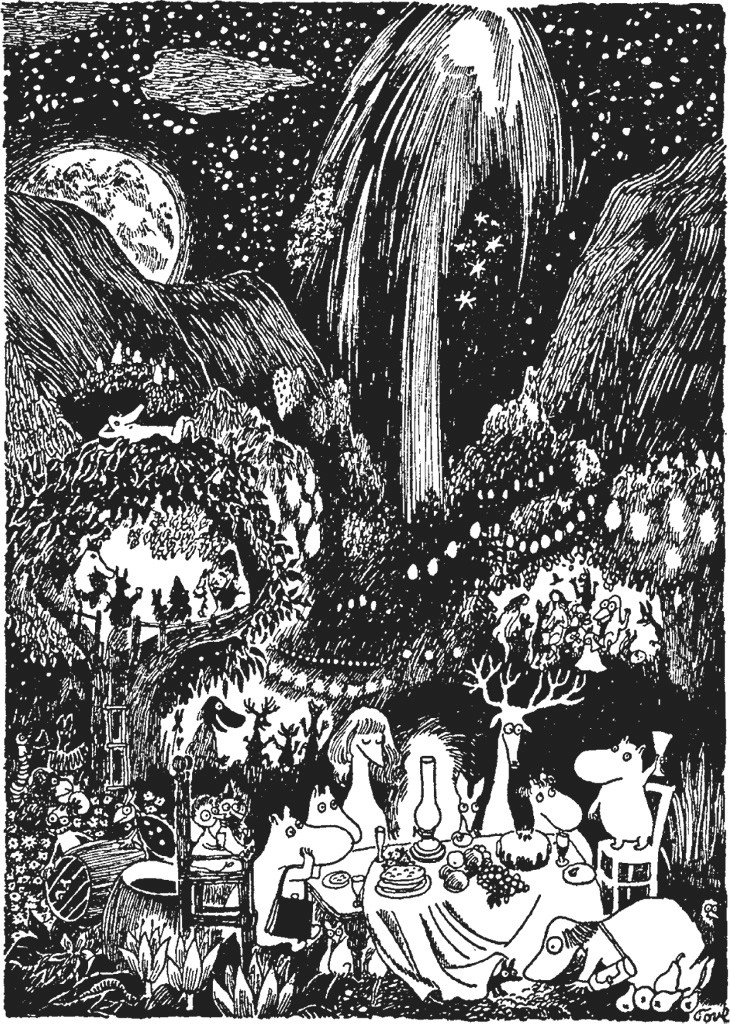
\includegraphics[width=451pt,height=633pt]{_34.jpg}
\caption{}
\label{_34}
\end{figure}

Jen la arĝenta fontano ekŝprucis, jen ekblovis la bengala neĝoŝtormo super la arbopintoj! Kaj laŭ la ĝardenpado la patro de Mumintrolo alrulis barelegon kun ruĝa vinpunĉo. Ĉiuj alkuris kun siaj glasoj kaj Muminpatro plenigis ĉiujn, tasojn kaj bovlojn, betulŝelajn ujojn, konkojn kaj folikornetojn.

``Je Tofslo kaj Vifslo!'' tostis la tuta Muminvalo. ``Hura', hura', hura'!''

``Huraslo!'' kriis Tofslo kaj Vifslo tostante unu kun la alia.

Poste Mumintrolo suriris seĝon kaj diris: ``Nun mi proponas toston je Snufmumriko kiu ĉi-nokte vagas suden, sola, sed certe same feliĉa kiel ni. Ni deziru al li bonan tendejon kaj malpezan koron!''

Kaj refoje la tuta valo levis siajn glasojn.

``Vi parolis bone,'' diris Snorkfraŭlino kiam Mumintrolo residiĝis.

``Nu, jes,'' diris Mumintrolo modeste. ``Sed mi elpensis ĝin antaŭe!''

Sed Muminpatro elportis la muzikan skatolon en la ĝardenon kaj alkonektis grandegan laŭtparolilon. En unu momento la tuta valo pleniĝis de danco, saltado, tretado, svingado, flirtado. La arbospiritoj dancis enaere kun fluganta hararo, kaj rigidkruraj musoparoj ronde dancis en la laŭboj.

``Ĉu vi permesas?'' diris Mumintrolo kun riverenco al Snorkfraŭlino.

Sed kiam li rigardis supren li ekvidis brilan randon super la arbopintoj.

Tio estis la aŭgusta luno.

Pli granda ol iam ĝi ŝvebis antaŭen, oranĝe flava kaj iom fadenmontra ĉe la rando kvazaŭ konfitita abrikoto. La lunbrilo ege mistere falis sur Muminvalon kiu pleniĝis de lumo kaj ombro.

``Ĉi-nokte eĉ eblas vidi la lunajn kraterojn,'' diris Snorkfraŭlino. ``Rigardu!''

`Tie devas esti terure dezerte,' pensis Mumintrolo. `Kompatinda sorĉisto kiu vagadas tie supre serĉante!'

``Se ni havus bonan lornon ni kredeble povus ekvidi lin,'' diris Snorkfraŭlino.

``Jes,'' diris Mumintrolo. ``Sed nun ni dancu!''

Kaj la festeno daŭris kun kreskanta forto.

``Ĉu vi estas lacsla?'' demandis Vifslo.

``Tutsle ne,'' diris Tofslo. ``Mi pripenslas. Ĉiuj estas tiel afabslaj al ni. Ni devslus iom ĝojigsli ilin!''

Tofslo kaj Vifslo kelkan tempon interflustris, kapjesis kaj ree flustris.

Poste ili rampis ĝis sia sekreta loko. Kiam ili reelvenis, ili kunportis la valizon.
\sectionbreak
Estis sufiĉe longe post noktomezo kiam la tuta ĝardeno subite pleniĝis de rozruĝa lumo. Ĉiuj ĉesis danci pensante ke tio estas nova artfajraĵo.

Sed tio estis nur Tofslo kaj Vifslo kiu malfermis sian valizon. La Reĝa Rubeno kuŝis surherbe lumante, pli bela ol iam. La fajroj, lanternoj, eĉ la luno paliĝis kaj perdis sian brilon. Silente kaj ravite ĉiuj kolektiĝis ĉirkaŭ la flamanta gemo en pli kaj pli grandaj kaj densaj aroj.

``Imagu ke troviĝas io tiel bela,'' ekkriis la patrino de Mumintrolo.

Kaj Snif profunde suspiris kaj diris: ``Feliĉaj Tofslo kaj Vifslo!''

\begin{figure}[htbp]
\centering
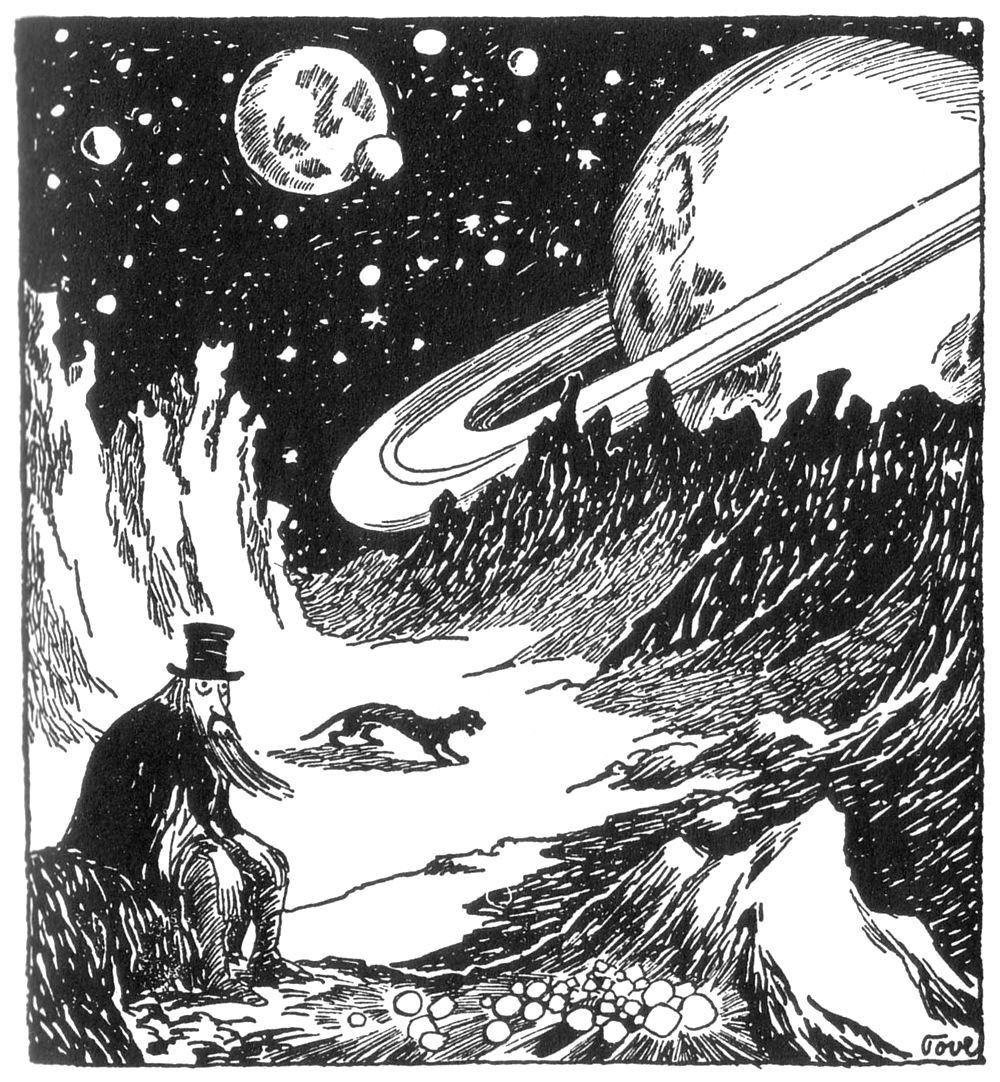
\includegraphics[width=425pt,height=460pt]{_35.jpg}
\caption{}
\label{_35}
\end{figure}

Sed la Reĝa Rubeno lumis kvazaŭ ruĝa okulo kontraŭ la nokte malluma tero, kaj supre sur la luno la sorĉisto ekvidis ĝin. Li jam rezignis plu serĉi kaj sidis laca kaj malĝoja sur la rando de kratero ripozante dum lia nigra pantero dormis iom fore.

La sorĉisto tuj komprenis kion signifas la ruĝa punkto sube surtere. Ĝi estis la plej granda rubeno de la mondo, la Reĝa Rubeno, kiun li serĉadis de plurcent jaroj! Li salte stariĝis kaj kun ardaj okuloj gapis al la tero surmetante la gantojn kaj fiksante la mantelon surŝultre. La juveloj kiujn li kolektis en ĝi li lasis fali sur la grundon -- la sorĉisto zorgis nur pri unu sola gemo, tiu kiun li post malpli ol duonhoro tenos enmane.

La pantero ĵetis sin en la aeron kun sia mastro surdorse.

Pli rapide ol la lumo ili pelis sin antaŭen tra la universo. Siblantaj meteoroj tranĉis ilian vojon, stela polvo fiksiĝis en la mantelo de la sorĉisto kvazaŭ blovata neĝo.

Sub li la ruĝa fajrero radiis pli kaj pli intense. Li direktis sin rekte kontraŭ Muminvalon kaj per lasta mola salto la pantero surteriĝis sur la monton.

La loĝantoj de Muminvalo ankoraŭ sidis silente kontemplante la Reĝan Rubenon. Ili imagis vidi en ĝiaj flamoj ĉion plej belan, kuraĝan kaj bonan kion ili iam pensis kaj spertis, kaj ili ekemis refoje pensi kaj sperti tion. Mumintrolo memoris sian noktan vagadon kun Snufmumriko, kaj Snorkfraŭlino pensis pri kiel fiere ŝi konkeris la lignan reĝinon. Kaj la patrino de Mumintrolo imagis refoje kuŝi sur la mola sablo en sunbrilo vidante la ĉielon inter la balanciĝantaj kapoj de sablaj diantoj.

Ĉiu el ili estis fore en io memorata. Kaj tial ili ĉiuj saltetis kiam blanka museto kun ruĝaj okuloj eliĝis el la ombro kaj plandis antaŭen kontraŭ la Reĝan Rubenon. Post li sekvis plennigra kato, kiu kuŝigis sin surherben.

Laŭ tio kion oni sciis neniu blanka muso loĝis en Muminvalo, nek nigra kato.

``Kateto, kateto!'' logis la hemulo.

Sed la kato nur fermis la okulojn kaj eĉ ne zorgis respondi.

``Bonan vesperon, kuzo!'' diris la arbara rato.

La blanka muso rigardis ŝin per siaj ruĝaj okuloj, longan, malgajan rigardon.

Muminpatro alpaŝis kun du tasoj por regali la novalvenintojn per vinpunĉo, sed ili ignoris lin.

Certa malgajeco disvastiĝis en la valo, oni flustris kaj miris. Tofslo kaj Vifslo maltrankviliĝis, reenmetis la rubenon en la valizon kaj fermis la kovrilon. Sed kiam ili volis forporti la valizon, la blanka muso ekstaris sur la postaj piedoj kaj kreskis.

Li iĝis preskaŭ same granda kiel la mumindomo. Li iĝis la sorĉisto kun blankaj gantoj kaj ruĝaj okuloj, kaj kiam li plenkreskis li sidiĝis sur la herbojn rigardante Tofslon kaj Vifslon.

``Malbelsla virslo, forirslu!'' diris Vifslo.

``Kie vi trovis la Reĝan Rubenon?'' demandis la sorĉisto.

``Zorgslu viajn proprajn aferslojn!'' diris Tofslo.

Neniu iam ajn vidis Tofslon kaj Vifslon tiel kuraĝaj.

``Mi serĉas ĝin de tricent jaroj,'' diris la sorĉisto. ``Mi zorgas pri nenio alia en la tuta mondo!''

``Samsle farslas ni!'' diris Vifslo.

``Vi ne povas forpreni de ili la Reĝan Rubenon,'' diris Mumintrolo. ``Ĝi estas honeste aĉetita de la morho! Sed Mumintrolo diris nenion pri tio ke ĝi estas aĉetita per la malnova ĉapelo de la sorĉisto (cetere li ja surhavis novan).''

``Donu al mi ion refortigan,'' diris la sorĉisto. ``Ĉi tio komencas ronĝi miajn nervojn.''

Muminpatrino tuj alkuris kun patkuko kaj konfitaĵo kaj donis al li grandan teleron.

Dum la sorĉisto manĝis ĉiuj kuraĝis iomete alproksimiĝi. Iu kiu manĝas patkukon kun konfitaĵo ne povas esti tiel terure danĝera. Eblas paroli kun li.

``Ĉu bongustslas?'' demandis Tofslo.

``Jes dankon,'' diris la sorĉisto. ``Mi ne ricevis patkukon dum la lastaj okdek kvin jaroj!''

Ĉiuj tuj kompatis lin kaj eĉ pli alproksimiĝis.

Kiam la sorĉisto finmanĝis li viŝis siajn lipharojn kaj diris: ``Mi ne povas forpreni de vi la Reĝan Rubenon, ĉar kio estas aĉetita devas esti aĉetita denove aŭ donacita. Ĉu vi ne povus vendi ĝin al mi por, ni diru du diamantaj montoj kaj valo plena de miksitaj gemoj?''

``Nenislam!'' diris Tofslo kaj Vifslo.

La sorĉisto suspiris kaj dum kelka tempo sidis pensante kun malgaja mieno.

Poste li diris: ``Lasu la festenon daŭri. Mi iom sorĉos por vi. Ĉiu ricevos sian propran sorĉon. Bonvolu deziri! Unue la mumingesinjoroj.''

La patrino de Mumintrolo iom hezitis. ``Ĉu estu aĵoj videblaj, ŝi demandis, aŭ ideoj? Se vi komprenas kion mi celas.''

``Certe,'' diris la sorĉisto. ``Aĵoj kompreneble estas pli facilaj, sed verŝajne ankaŭ ideoj eblos.''

``Do mi tre dezirus ke Mumintrolo ne plu malĝoju pro la Snufmumriko,'' diris Muminpatrino.

``Mi ne sciis ke tio vidiĝas,'' diris Mumintrolo ruĝiĝante.

Sed la sorĉisto iom svingis sian mantelon, kaj tuj la melankolio forflugis el la koro de Mumintrolo. Lia sopiro iĝis nura espero, kaj tio estis multe pli agrabla sento.

''Mi havas ideon! vokis Mumintrolo. ``Kara sorĉisto, lasu la tutan manĝotablon kun ĉio sur ĝi flugi ĝis Snufmumriko, kie ajn li nun troviĝas!''

En la sama momento la tablo altiĝis inter la arbopintoj kaj ŝvebis suden kun patkuko kaj konfitaĵo, kun fruktoj, floroj, vinpunĉo kaj bombonoj, kaj kun la libro de la moskorato, kiun li metis sur angulon de la tablo.

\begin{figure}[htbp]
\centering
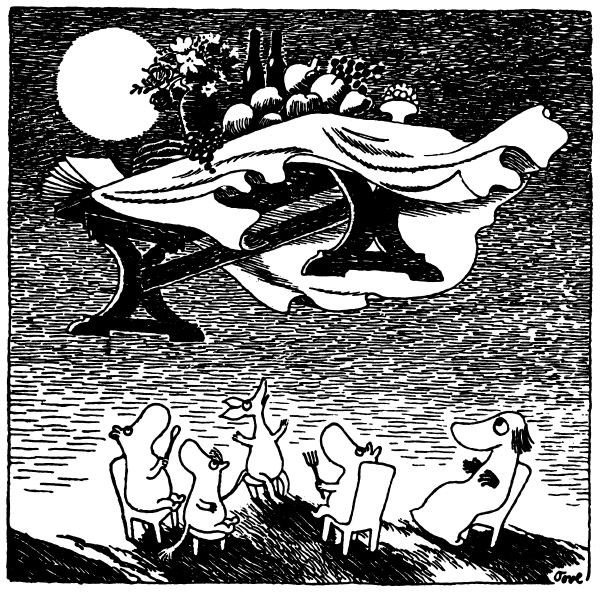
\includegraphics[width=449pt,height=445pt]{_36.jpg}
\caption{}
\label{_36}
\end{figure}

``Ne, kio nun!?'' diris la moskorato. ''Bonvolu tuj resorĉi al mi mian libron!

Farite ne refariĝas! diris la sorĉisto. Sed vi ricevos novan libron,

sinjoro. Bonvolu!''

```Pri la neceso de ĉio','' legis la moskorato. ``Sed tio ja estas tute erare! Tiu kiun mi havis temis pri la neneceso de ĉio!''

Sed la sorĉisto nur ridis.

``Nun ŝajne estas mia vico,'' diris la patro de Mumintrolo. ``Sed estas tre malfacile elekti! Mi pensis pri amaso da aferoj kaj neniu estas vere bona. Vitrodomon estas pli amuze mem fari. Same boateton. Cetere mi jam havas la plej multajn aferojn!''

``Sed eble vi tute ne bezonas deziri,'' proponis Snif. ``Vi povus anstataŭe lasi min deziri dufoje?''

``Nu,'' diris Muminpatro. ``Sed kiam oni esceptokaze \emph{rajtas} deziri{\ldots}''

``Provu iomete rapidi,'' diris la patrino de Mumintrolo. ``Deziru vere belan kovrilon por viaj memoroj!''

``Jes, tio estos bona,'' diris la patro ĝoje. ``Ĉiuj aŭdigis admirajn vokojn kiam la sorĉisto transdonis perlogarnitan kovrilon el oro kaj ruĝa marokeno.''

``Nun mi!'' vokis Snif. ``Propran boaton! Boaton kiel konko kun purpuraj veloj! La masto estu el jakarando kaj ĉiuj remilingoj el smeraldoj!''

``Tio ne estas malmulte,'' diris la sorĉisto amike svingante la mantelon.

Ĉiuj retenis la spiron, sed neniu boato vidiĝis.

``Ĉu estiĝis nenio?'' diris Snif elrevigite.

``Certe estiĝis,'' diris la sorĉisto. ``Sed kompreneble mi metis ĝin malsupre ĉe la strando. Vi trovos ĝin tie morgaŭ.''

``Ĉu kun smeraldaj remilingoj?'' demandis Snif.

``Certe. Kvar kaj unu rezerva,'' diris la sorĉisto. ``Nun la sekva.''

``Nu,'' diris la hemulo. ``Se diri la veron mi rompis la botanikan fosileton kiun mi pruntis de la snorko. Do mi absolute bezonus novan.''

Kaj li genufleksis\footnote{La hemulo genufleksas ĉar aspektas iom stulte kapklini en robo. -- \emph{Noto de la aŭtoro}.} bonedukite kiam la sorĉisto transdonis la novan botanikan fosileton.

``Ĉu ne estas lacige sorĉi?'' demandis Snorkfraŭlino.

``Ne pro ĉi tiel facilaj aferoj!'' diris la sorĉisto. ``Kaj kion deziras la eta fraŭlino?''

``Tio sendube estos pli malfacila,'' diris Snorkfraŭlino. ``Ĉu mi rajtas flustri?''

Kiam ŝi finflustris la sorĉisto mienis iom surprizite kaj demandis: ``Ĉu vi certas ke ili konvenos, fraŭlino?''

``Jes! Certe!'' spiris Snorkfraŭlino.

``Nu, bone do!'' diris la sorĉisto. ``Estu!''

En la sekva momento voko pro surprizo trairis la amason. Snorkfraŭlino staris antaŭ ili kun tute ŝanĝita aspekto.

``Kion vi faris al vi!?'' ekkriis Mumintrolo indigne.

``Mi deziris la okulojn de la ligna reĝino,'' diris Snorkfraŭlino. ``Vi ja trovis ŝin bela!''

``Jes, sed{\ldots}'' murmuris Mumintrolo malfeliĉe.

``Ĉu vi ne trovas ilin belaj?'' diris Snorkfraŭlino kaj ekploris.

\begin{figure}[htbp]
\centering
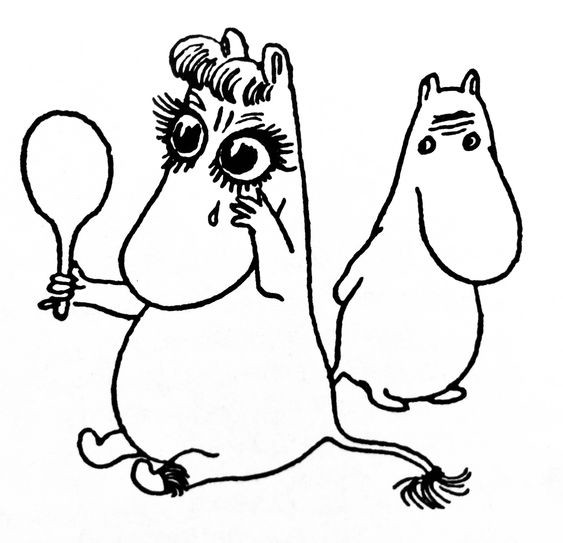
\includegraphics[width=122pt,height=120pt]{_37.jpg}
\caption{}
\label{_37}
\end{figure}

``Nu nu,'' diris la sorĉisto. ``Se tio ne estis bona do via frato povos deziri la malnovajn okulojn reen!''

``Jes, sed mi intencis ion tute alian,'' protestis la snorko. ``Mi ja ne kulpas se ŝi faras stultajn dezirojn!''

``Pri kio do vi pensis?'' demandis la sorĉisto.

Kalkulmaŝino! respondis la snorko. Maŝino kiu kalkulas ĉu aferoj estas justaj aŭ maljustaj, bonaj aŭ malbonaj.

``Tio estas tro malfacila,'' diris la sorĉisto skuante la kapon. ``Tion mi ne kapablas.''

``Nu, do maŝino kiu skribas,'' diris la snorko. ``Mia fratino ja vidas same bone per siaj novaj okuloj!''

``Jes, sed ŝi ne aspektas same bone,'' diris la sorĉisto.

``Karulo!'' ploris Snorkfraŭlino kiu trovis spegulon. ``Deziru miajn malnovajn okuletojn reen! Mi ja aspektas terure!''

``Nu,'' diris la snorko grandanime. ``Vi ricevos ilin pro la familia honoro.Sed mi esperas ke vi post ĉi tio estos iom malpli vanta.''

Snorkfraŭlino denove rigardis en la spegulon kaj ekkriis pro ĝojo. Ŝiaj malnovaj hejmecaj okuloj revenis sialoken, sed la okulharoj efektive iomete plilongiĝis! Ŝi ĝojradie brakumis sian fraton vokante: ``Karulo! Dolĉulo! Vi ricevos maŝinon kiu skribas kiel printempan donacon de mi!''

``Ej,'' diris la snorko embarasite. ``Oni ne kisu kiam iuj rigardas. Mi ne eltenis vidi vin en tiu terura aspekto, jen la tuta afero.''

``Bone, nun restas nur Tofslo kaj Vifslo el la domanoj,'' diris la sorĉisto.

Vi ricevos unu komunan deziron ĉar ne eblas ja distingi vin!

``Ĉu vi mem do nenislon dezirslos?'' scivolis Tofslo.

``Mi ne povas,'' diris la sorĉisto malgaje. ``Mi povas nur deziri por aliaj kaj transformi min en diversajn aferojn!''

Tofslo kaj Vifslo gapis al li. Poste ili kunigis la kapojn kaj longe interflustris.

Post tio Vifslo diris solene: ``Ni decidslis dezirsli por vi, ĉar vi estas bonsla. Ni volas rubenslon kiu estas same grandsla kaj belsla kiel la nisla!''

Ĉiuj jam vidis la sorĉiston ridi, sed neniu kredis ke li povas rideti.

Nun li ridetis per la tuta vizaĝo. Li tiom ĝojis ke tio vidiĝis ĉie ĉe li, ĉe la oreloj, ĉapelo, botoj! Sen unu vorto li svingis sian mantelon super la herboj -- kaj vidu! Refoje la ĝardeno pleniĝis de rozruĝaj flamoj, jen kuŝis antaŭ ili ĝemelo de la Reĝa Rubeno, Reĝina Rubeno.

``Nun vi ĝojslas, ĉu ne?'' diris Tofslo.

\emph{''Certe} mi ĝojas!'' vokis la sorĉisto kaj tenere levis la brilantan valoraĵon en sia mantelo. ``Nun ĉiu eta knito kaj arbara rato kaj besteto en la tuta valo rajtas deziri kion li, ŝi aŭ ĝi volas! Mi plenumos viajn dezirojn ĝis matene, ĉar antaŭ la sunleviĝo mi revenu hejmen.''

Kaj nun estiĝis vera festeno!

Antaŭ la sorĉisto serpentis longa vico da pepantaj, ridantaj, murmurantaj kaj vokantaj arbaruloj kiuj ĉiuj volis ke ilia deziro plenumiĝu. Kiu deziris stulte rajtis refari tion ĉar la sorĉisto estis je bonega humoro. La danco rekomenciĝis kaj novaj ĉarumoj da patkuko estis trenataj sub la arbojn. La hemulo ekbruligis artfajraĵojn senĉese kaj Muminpatro elportis siajn memorojn en ilia bela kovrilo kaj laŭtlegis pri sia infanaĝo.

Neniam antaŭe oni tiel ege festenis en Muminvalo!

Ho, feliĉo, kiam oni formanĝis ĉion, eltrinkis ĉion, priparolis ĉion kaj dancis siajn krurojn lacaj, reiri hejmen en la silenta horo antaŭ la sunleviĝo por dormi!

La sorĉisto flugas ĝis la fino de l' mondo kaj la musino enrampas sub sian herbotufon, sed ambaŭ estas same feliĉaj.

Kaj eble plej feliĉa estas Mumintrolo kiu kun sia panjo reiras hejmen tra la ĝardeno. La nokto ĝuste paliĝas kiam la luno en la tagiĝo kaj matena vento venanta el la maro iomete movas la arbojn. Nun la malvarmeta aŭtuno enpaŝas en Muminvalon. Ĉar alie ja ne povus refariĝi printempo.

\begin{figure}[htbp]
\centering
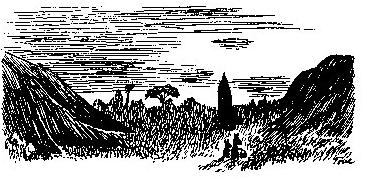
\includegraphics[keepaspectratio,width=\textwidth,height=0.75\textheight]{_38.jpg}
\caption{}
\label{_38}
\end{figure}

%
%	MultiMarkdown default footer
%


% Back Matter
\if@mainmatter
	we're in main
	\backmatter
\fi


% Bibliography

\ifx\bibliocommand\undefined
\else
	\bibliographystyle{\bibliostyle}
	\bibliocommand
\fi



% Glossary
\printglossaries


% Index
\printindex


\end{document}
